\documentclass[12pt,thmsa]{article}

%maths
\usepackage{amsmath}   % \sideset
\usepackage{amsthm}    % for proof
\usepackage{amsfonts}  % for \mathbb
\usepackage{mathrsfs}  % for Ralph Smith's Formal Script Font
\usepackage[mathscr]{euscript} %redefine the \mathcal command to use Euler script
\usepackage{amssymb}   % \varnothing, \bigstar, \blacksquare, \clubsuit, \blacktriangleright, \diamondsuit, \spadesuit, \dagger, \checkmark
\usepackage{optidef}   % for optimization definition

%algorithms
\usepackage{algpseudocode}% http://ctan.org/pkg/algorithmicx
\usepackage[ruled,vlined,linesnumbered]{algorithm2e} % For algorithm
%\usepackage{algorithm}% http://ctan.org/pkg/algorithms % conflict with algorithm2e

%tables
\usepackage{booktabs}  % Allows the use of \toprule, \midrule and \bottomrule in tables
\usepackage{multirow}
\usepackage{multicol}
\usepackage{tabularx}
\usepackage[table]{xcolor} % For \cellcolor
\usepackage[export]{adjustbox}

%figures
\usepackage{graphicx}  % Allows including images
\usepackage{float}     % Force figure placement in text with [H]

%tikzpicture
\usepackage{tikz}
\usepackage{scalerel}
\usepackage{pict2e}
\usepackage{tkz-euclide}
\usetikzlibrary{matrix}
\usetikzlibrary{shapes, positioning}
\usetikzlibrary{calc}
\usetikzlibrary{patterns, arrows.meta}
\usetikzlibrary{shadows}
\usetikzlibrary{external}
\usetikzlibrary{3d}

%pgfplots
\usepackage{pgfplots}
\pgfplotsset{compat=newest}
\usepgfplotslibrary{statistics}
\usepgfplotslibrary{fillbetween}

%colors
\usepackage{color}     % color
\usepackage[colorinlistoftodos]{todonotes}

%other
\usepackage{cancel}
\usepackage{enumitem}
\setlist[itemize]{leftmargin=*} % global option, remove the indentation for a specific list
\usepackage{textcase}  % \MakeTextUppercase
\renewcommand{\qedsymbol}{$\blacksquare$} % change the QED symbol to a filled square
\usepackage{hyperref}
\usepackage{tocloft}

%layout
\usepackage{geometry}
\usepackage{fancyhdr}   % Fancy Headers
\usepackage{setspace}   % Include the setspace package


%------------------------------------------------------%
%              Create Center Title Page                              %
%------------------------------------------------------%
\usepackage{titling}
\renewcommand\maketitlehooka{\null\mbox{}\vfill}
\renewcommand\maketitlehookd{\vfill\null}

\graphicspath{ {./Figure/} }

\geometry{
	a4paper,
	total={170mm,257mm},
	left=20mm,
	right=20mm,
	top=20mm,
}

% Linhui added for newly defined color
\definecolor{forestgreen}{RGB}{34,139,34}


% Linhui added for Expectation and Variance
\newcommand{\Exp}{{\mathbb E}\! }
\newcommand{\Var}{\mbox{Var}\! }

% Linhui added for rename the command for empty set.
\let\oldemptyset\emptyset
\let\emptyset\varnothing


%------------------------------------------------------%
\makeatletter
\def\maketitle{%
	\par
	\hrule height 1.5pt\vspace{1ex}
	\par\noindent
	
	\begin{minipage}{0.5\textwidth}
		\scshape
		Purdue University $\cdot$ ece 58000 \\[1ex]
		Optimization Methods \\
		Prof. Żak
	\end{minipage}
	\begin{minipage}{0.45\textwidth}
		\raggedleft
		\MakeTextUppercase{{\@title}}\\[0.3ex] % 0.2ex height space between two line
		\textit{\@author}\\[0.2ex]
		\textit{August 1, 2022}
	\end{minipage}
	\par\vspace{1ex}
	\hrule height 1.5pt\vspace{1ex}
	\par
}
\makeatother

\author{Linhui Xie}
\title{Review of Qualify Exam}
%------------------------------------------------------%

\begin{document}
	\tableofcontents
	\newpage
	
% Part 1: Math Review
\maketitle
%------------------------------------------------------%
%------------------------------------------------------%
\section{Quadratic Forms \medskip}
%------------------------------------------------------%
%------------------------------------------------------%

%------------------------------------------------------%
\subsection{Concept}
\begin{itemize}
	\item \(f: \mathbb{R}^{n} \rightarrow \mathbb{R}\) is a \underline{quadratic} function if

	\begin{equation*}
		f(\boldsymbol{x})=\boldsymbol{x}^{T} \boldsymbol{Q} \boldsymbol{x}+\boldsymbol{b}^{T} \boldsymbol{x}+c,
	\end{equation*}
	
	where \(\boldsymbol{Q}\) is {\color{black}symmetric}.

	\item \(\boldsymbol{Q}\) is symmetric if \(\boldsymbol{Q}=\boldsymbol{Q}^{\top}\).
	
	\item A symmetric matrix \(\boldsymbol{Q}\) is said to be \underline{positive definite} (p.d.) if \(\boldsymbol{x}^{\top} \boldsymbol{Q} \boldsymbol{x}>0\) for {\color{black}all nonzero} vectors \(\boldsymbol{x}\).
	
	\item It is \underline{positive semi-definite} (p.s.d.) if \(\boldsymbol{x}^{\top} \boldsymbol{Q} \boldsymbol{x} \geq 0\) for {\color{black}all} \(\boldsymbol{x}\).
	
	\item Similarly, \underline{negative definite} (n.d.) and \underline{negative semi-definite} (n.s.d.),  if \(\boldsymbol{x}^{\top} \boldsymbol{Q} \boldsymbol{x}<0\) for {\color{black}all nonzero} vectors \(\boldsymbol{x}\), or \(\boldsymbol{x}^{\top} \boldsymbol{Q} \boldsymbol{x} \leq 0\) for {\color{black}all} \(\boldsymbol{x}\), respectively.
	
	\item If a  \(n \times n\) matrix \(\boldsymbol{Q}_{0}\) is not symmetric, we can always replace it with the symmetric, as

	\begin{equation*}
		\begin{gathered}
			\boldsymbol{Q}=\boldsymbol{Q}^{T}=\frac{1}{2}\left(\boldsymbol{Q}_{0}+\boldsymbol{Q}_{0}^{T}\right), \\
			\boldsymbol{x}^{T} \boldsymbol{Q} \boldsymbol{x}=\boldsymbol{x}^{T} \boldsymbol{Q}_{0} \boldsymbol{x}=\boldsymbol{x}^{T}\left(\frac{1}{2} \boldsymbol{Q}_{0}+\frac{1}{2} \boldsymbol{Q}_{0}^{T}\right) \boldsymbol{x}.
		\end{gathered}
	\end{equation*}
	
	\item The leading principal minors of matrix \(\boldsymbol{Q}\) are,
	
	\begin{equation*}
		\begin{gathered}
			\Delta_{1}=q_{11}, \quad \Delta_{2}=\operatorname{det}\left[\begin{array}{ll}
				q_{11} & q_{12} \\
				q_{21} & q_{22}
			\end{array}\right], 
			\Delta_{3}=\operatorname{det}\left[\begin{array}{lll}
				q_{11} & q_{12} & q_{13} \\
				q_{21} & q_{22} & q_{23} \\
				q_{31} & q_{32} & q_{33}
			\end{array}\right], \quad \ldots
		\end{gathered}
	\end{equation*}

	\item For an \(n \times n\) symmetric real matrix \(\boldsymbol{Q}\),
	\begin{equation*}
		\begin{aligned}
			\boldsymbol{Q} \text{ positive-definite }  &  \Longleftrightarrow \quad \boldsymbol{x}^{\top} \boldsymbol{Q} \boldsymbol{x}>0 \text { for all } \boldsymbol{x} \in \mathbb{R}^n \backslash\{\boldsymbol{0}\}, \\
			\boldsymbol{Q}  \text{ positive semi-definite } & \Longleftrightarrow \quad \boldsymbol{x}^{\top} \boldsymbol{Q} \boldsymbol{x} \geq 0 \text{ for all } \boldsymbol{x} \in \mathbb{R}^n, \\
			\boldsymbol{Q} \text { negative-definite } & \Longleftrightarrow \quad \boldsymbol{x}^{\top} \boldsymbol{Q} \boldsymbol{x}<0 \text { for all } \boldsymbol{x} \in \mathbb{R}^n \backslash\{\boldsymbol{0}\}, \\
			\boldsymbol{Q} \text { negative semi-definite } &\Longleftrightarrow \quad \boldsymbol{x}^{\top} \boldsymbol{Q} \boldsymbol{x} \leq 0 \text { for all } \boldsymbol{x} \in \mathbb{R}^n.
		\end{aligned}
	\end{equation*}
	
	\item For an \(n \times n\) Hermitian complex matrix \(\boldsymbol{Q}\),
	\begin{equation*}
		\begin{aligned}
			\boldsymbol{Q} \text{ positive-definite }, \boldsymbol{Q} \succ 0 &  \Longleftrightarrow \quad
			\boldsymbol{x}^{\top} \boldsymbol{Q} \boldsymbol{x}>0 \text { for all } \boldsymbol{x} \in \mathbb{C}^n \backslash\{\boldsymbol{0}\}, \\
			\boldsymbol{Q}  \text{ positive semi-definite }, \boldsymbol{Q}  \succeq 0 & \Longleftrightarrow \quad \boldsymbol{x}^{\top} \boldsymbol{Q} \boldsymbol{x} \geq 0 \text{ for all } \boldsymbol{x} \in \mathbb{C}^n, \\
			\boldsymbol{Q} \text { negative-definite }, \boldsymbol{Q}  \prec 0 & \Longleftrightarrow \quad
			\boldsymbol{x}^{\top} \boldsymbol{Q} \boldsymbol{x}<0 \text { for all } \boldsymbol{x} \in \mathbb{C}^n \backslash\{\boldsymbol{0}\}, \\
			\boldsymbol{Q} \text { negative semi-definite }, \boldsymbol{Q}  \preceq 0 &\Longleftrightarrow \quad \boldsymbol{x}^{\top} \boldsymbol{Q} \boldsymbol{x} \leq 0 \text { for all } \boldsymbol{x} \in \mathbb{C}^n.
		\end{aligned}
	\end{equation*}
	
	
	\item[\(\spadesuit\)] \(\mathscr{THEOREM}\) 3.6 Sylvester's Criterion. A quadratic form (\(\boldsymbol{Q}\) is symmetric) \(\boldsymbol{x}^{\top} \boldsymbol{Q} \boldsymbol{x}, \boldsymbol{Q}=\boldsymbol{Q}^{\top}\), is positive definite if and only if the leading principal minors of \(\boldsymbol{Q}\) are positive.

	\item[\(\spadesuit\)] \(\mathscr{THEOREM}\) 3.7  A symmetric matrix \(\boldsymbol{Q}\) is positive definite (or positive semidefinite) if and only if all eigenvalues of \(\boldsymbol{Q}\) are positive (or non-negative).

	\item A necessary condition for a real quadratic form to be positive semi-definite is that the leading principal minors be nonnegative. However, it is not a sufficient condition.
	
	\item A real quadratic form is positive semi-definite if and only if all principal minors are non-negative.
	
\end{itemize}



%------------------------------------------------------%
\subsection{Examples}
%------------------------------------------------------%
Example 1: (1) Given set \(\Omega=\left\{\boldsymbol{x} \in \mathbb{R}^{3}\right\}\),

(2) \(\Omega=\left\{\boldsymbol{x} \in \mathbb{R}^{3}: x_{1}+x_{3}=0, x_{1}+x_{2}+x_{3}=0\right\}\), is the quadratic form,

\begin{equation*}
	f(\boldsymbol{x})=\boldsymbol{x}^{\top} \boldsymbol{Q} \boldsymbol{x}=\boldsymbol{x}^{\top}\left[\begin{array}{ccc}
		5 & 3 & 0 \\
		0 & 0 & 5 \\
		7 & 3 & 1
	\end{array}\right] \boldsymbol{x},
\end{equation*}

p.d, p.s.d, n.d, n.s.d, or indefinite on \(\mathbb{R}^{3}\)?

\noindent
\textbf{Short answer:}

(1) Notice that \(\boldsymbol{Q}\) is not symmetric, first convert it to standard form

\begin{equation*}
	f(\boldsymbol{x})=\frac{1}{2} \boldsymbol{x}^{\top}\left(\boldsymbol{Q}+\boldsymbol{Q}^{\top}\right) \boldsymbol{x}=\frac{1}{2} \boldsymbol{x}^{\top}\left[\begin{array}{ccc}
		10 & 3 & 7 \\
		3 & 0 & 8 \\
		7 & 8 & 2
	\end{array}\right] \boldsymbol{x} .
\end{equation*}

Since leading principal minors \(10>0\) and \(\operatorname{det}\left[\begin{array}{cc}10 & 3 \\ 3 & 0\end{array}\right]<0, f(\boldsymbol{x})\) is indefinite on \(\mathbb{R}^{3}\).


(2) Let \(\boldsymbol{x}=\left[\begin{array}{lll}a & 0 & -a\end{array}\right]^{\top}, a \in \mathbb{R}\), and \(a \neq 0\). Then \(f(\boldsymbol{x})=-a^{2}<0\). Therefore, \(f(\boldsymbol{x})\) is negative definite on the set \(\Omega\).


%------------------------------------------------------%
\bigskip
\noindent
Example 2: Is the matrix

\begin{equation*}
	\boldsymbol{Q}=\left[\begin{array}{ccc}
		\alpha^{4} & \alpha^{3} & \alpha^{2} \\
		\alpha^{3} & \alpha^{2} & \alpha^{1} \\
		\alpha^{2} & \alpha^{1} & 1
	\end{array}\right]
\end{equation*}

where \(\alpha \in \mathbb{R}\), p.d, p.s.d, n.d, n.s.d or indefinite?

\noindent
\textbf{Short answer:}
Let \(\boldsymbol{v}=\left[\begin{array}{lll}\alpha^{2} & \alpha^{1} & 1\end{array}\right]^{\top}\). Then \(\boldsymbol{Q}=\boldsymbol{v} \boldsymbol{v}^{\top}\) and \(\boldsymbol{x}^{\top} \boldsymbol{Q} \boldsymbol{x}=\boldsymbol{x}^{\top} \boldsymbol{v} \boldsymbol{v}^{\top} \boldsymbol{x}=\left(\boldsymbol{x}^{\top} \boldsymbol{v}\right)^{2} \geq 0\). Therefore, \(\boldsymbol{Q}\) is positive semi-definite.


%------------------------------------------------------%
\bigskip
\noindent
Example 3: Find the range of the coefficient \(\beta\) for the function:

\begin{equation*}
	f\left(x_{1}, x_{2}, x_{3}\right)=2 x_{1} x_{3}-x_{1}^{2}-x_{2}^{2}-5 x_{3}^{2}-2 \beta x_{1} x_{2}-4 x_{2} x_{3}
\end{equation*}

is negative semi-definite.

\noindent
\textbf{Short answer:}
If \(f(\boldsymbol{x})\) is n.s.d, then \(-f(\boldsymbol{x})\) is p.s.d.

\begin{equation*}
	-f(\boldsymbol{x})=\boldsymbol{x}^{\top} \boldsymbol{Q} \boldsymbol{x}=\boldsymbol{x}^{\top}\left[\begin{array}{ccc}
		1 & \beta & -1 \\
		\beta & 1 & 2 \\
		-1 & 2 & 5
	\end{array}\right] \boldsymbol{x} .
\end{equation*}

Let \(\operatorname{det}\left[\begin{array}{ll}1 & \beta \\ \beta & 1\end{array}\right]=1-\beta^{2} \geq 0\) and \(\operatorname{det}(\boldsymbol{Q})=-5 \beta^{2}-4 \beta \geq 0\), we have \(\beta \in\left[-\frac{4}{5}, 0\right]\).

\bigskip

\noindent
[Ref]: Edwin K.P. Chong, Stanislaw H. Żak, ``PART I MATHEMATICAL REVIEW" in ``An introduction to optimization", 4th Edition, John Wiley and Sons, Inc. 2013.

%------------------------------------------------------%
%------------------------------------------------------%
\section{Gradient and Hessian}
%------------------------------------------------------%
%------------------------------------------------------%

%------------------------------------------------------%
\subsection{Concept}
\begin{itemize}
	\item[({\bf{1}})] Given \(f: \mathbb{R} \rightarrow \mathbb{R}\), if the limit exists, the derivative of \(f\) is a function \(f^{\prime}: \mathbb{R} \rightarrow \mathbb{R}\) given by
	\[
	D_{x}(f(x)) = \frac{\mathrm{d} f}{\mathrm{d} x} = f^{\prime}(x)=\lim _{h \rightarrow 0} \frac{f(x+h)-f(x)}{h}.
	\]
	
	\item[({\bf{2}})] Given \(f: \mathbb{R}^{n} \rightarrow \mathbb{R}\), consider a scalar \( f(\boldsymbol{x}) = a_{1} x_{1}+a_{2} x_{2}+\cdots+a_{n} x_{n} =  \boldsymbol{a}^{\top} \boldsymbol{x}\).
	
	For \textbf{derivative} rule (2), 
	\[ 
	{\color{red}{D_{\boldsymbol{x}}}} { f(\boldsymbol{x}) } =
	{\color{black}{D(}}{ \boldsymbol{a}^{\top} \boldsymbol{x} }{\color{black})} 
	= 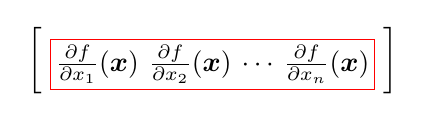
\begin{tikzpicture}[baseline=(current bounding box.center)]
		\matrix (m) [matrix of math nodes, inner sep=1.8pt, row sep=0pt, left delimiter={[},right delimiter={]}] {
			\frac{\partial f}{\partial x_1} (\boldsymbol{x}) & \frac{\partial f}{\partial x_2}(\boldsymbol{x}) & \cdots & \frac{\partial f}{\partial x_n}(\boldsymbol{x}) \\
		};
		\draw[red] (m-1-1.north west) rectangle (m-1-4.south east);
	\end{tikzpicture}
	=\left[\begin{array}{cccc}
		a_{1} & a_{2} &  \cdots & a_{n}
	\end{array}
	\right] = {\color{red}{ \boldsymbol{a}^{\top} }}.
	\]
	
	For \textbf{gradient} rule (2), \underline{if \(f: \mathbb{R}^{n} \rightarrow \mathbb{R}\) is differentiable}, then the \textit{gradient} of \(f\) is a function \(\nabla f: \mathbb{R}^{n} \rightarrow \mathbb{R}^{n}\) given by
	\[  {\color{blue}{\nabla}_{\boldsymbol{x}} } f(\boldsymbol{x})
	= 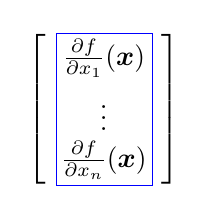
\begin{tikzpicture}[baseline=(current bounding box.center)]
		\matrix (m) [matrix of math nodes, inner sep=2pt, left delimiter={[},right delimiter={]}, nodes in empty cells] {
			\frac{\partial f}{\partial x_1} (\boldsymbol{x}) \\
			|[minimum height=0.5cm]|  \vdots \\
			\frac{\partial f}{\partial x_n} (\boldsymbol{x}) \\
		};
		\draw[blue] (m-1-1.north west) rectangle (m-3-1.south east);
	\end{tikzpicture}
	= \left[ \begin{array}{c} a_1  \\ \vdots \\ a_n \end{array} \right]
	= {\color{blue}{ \boldsymbol{a} }}
	= D_{\boldsymbol{x}} f(\boldsymbol{x}) ^{\top}.
	\] 
	
	\item[({\bf{3}})] Given \(\boldsymbol{g}: \mathbb{R} \rightarrow \mathbb{R}^m \), here \(t \in \mathbb{R} \) is a scalar. \(\boldsymbol{g}(t)\) is a column vector.
	\[
	\begin{aligned}
		\boldsymbol{g}(t) =
		\left[
		\begin{array}{c}
			g_{1}(t) \\
			\vdots \\
			g_{m}(t)
		\end{array}
		\right], \quad
		D_{t} \boldsymbol{g}(t) & =\left[
		\begin{aligned}
			\frac{\mathrm{d}}{\mathrm{d} t}g_{1}(t) \\
			\vdots \qquad \\
			\frac{\mathrm{d}}{\mathrm{d} t}g_{m}(t)
		\end{aligned}
		\right] =\left[\begin{array}{c}
			g_{1}^{\prime}(t) \\
			\vdots \\
			g_{m}^{\prime}(t)
		\end{array}\right].  \\
	\end{aligned}
	\]
	
	\item[({\bf{4}})] Consider \(\boldsymbol{g}: \mathbb{R}^{n} \rightarrow \mathbb{R}^m \),  here \( \boldsymbol{x} \in  \mathbb{R}^n \) is a vector. Since \(g_{i}(\boldsymbol{x})\) is a scalar, \(\boldsymbol{g}=\left[g_1, \ldots, g_m\right]^{\top} \), \(\boldsymbol{g}(\boldsymbol{x})\) is a column vector.
	\[
	\begin{aligned}
		\boldsymbol{g} \left( \boldsymbol{x} \right)=
		\left[
		\begin{array}{c}
			g_{1}( \boldsymbol{x} ) \\
			g_{2}( \boldsymbol{x} ) \\
			\vdots \\
			g_{m}( \boldsymbol{x} )
		\end{array}
		\right], 
		D_{\boldsymbol{x}} \boldsymbol{g}\left( \boldsymbol{x} \right) & =\left[
		\begin{array}{c}
			{ \color{red}D_{\boldsymbol{x}} } g_{1}\left( x_1,x_2,\cdots,x_n \right) \vspace{0.3cm} \\
			{ \color{red}D_{\boldsymbol{x}} } g_{2}\left( x_1,x_2,\cdots,x_n \right)  \\
			\vdots \\
			{ \color{red}D_{\boldsymbol{x}} } g_{m}\left( x_1,x_2,\cdots,x_n \right) 
		\end{array}
		\right]
		= 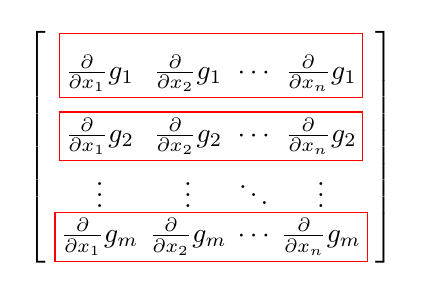
\begin{tikzpicture}[baseline=(current bounding box.center)]
			\matrix [matrix of math nodes, inner sep=2pt, left delimiter={[},right delimiter={]}] (m) {
				|[minimum height=1cm]| \frac{\partial}{\partial x_1} g_1 & \frac{\partial}{\partial x_2} g_1 & \cdots & \frac{\partial}{\partial x_n} g_1 \\
				\frac{\partial}{\partial x_1} g_2 & \frac{\partial}{\partial x_2} g_2 & \cdots & \frac{\partial}{\partial x_n} g_2 \\
				\vdots & \vdots & \ddots & \vdots \\
				\frac{\partial}{\partial x_1} g_m & \frac{\partial}{\partial x_2} g_m & \cdots & \frac{\partial}{\partial x_n} g_m \\
			};
			\draw[red] (m-1-1.north west) rectangle (m-1-4.south east);
			\draw[red] (m-2-1.north west) rectangle (m-2-4.south east);
			\draw[red] (m-4-1.north west) rectangle (m-4-4.south east);
		\end{tikzpicture}
		= \mathbf{J}.
	\end{aligned}
	\]
	The matrix \(\mathbf{J}\) is called the \underline{Jacobian matrix}, or derivative matrix, of function \(\boldsymbol{g}\).
	
	\item Note that, \( D \left( f(\boldsymbol{x}) \right)\) is spreading the derivative of the polynomials on the horizontal direction. The second derivative of \(f: \mathbb{R}^{n} \rightarrow \mathbb{R}\) (also called the Hessian of \(f\) ) is
	\[ D^{2} \left( f(\boldsymbol{x}) \right)
	= D \left(  D f \left( \boldsymbol{x} \right)^{\top} \right)
	= D(\nabla f(\boldsymbol{x}))
	= \left[\begin{array}{c}    
		D\left(\frac{\partial f}{ \color{forestgreen}{\partial x_{1}} }\right) \\    
		D\left(\frac{\partial f}{ \color{forestgreen}{\partial x_{2}} }\right) \\    
		\vdots \\    
		D\left(\frac{\partial f}{ \color{forestgreen}{\partial x_{n}} }\right)    
	\end{array}
	\right]
	=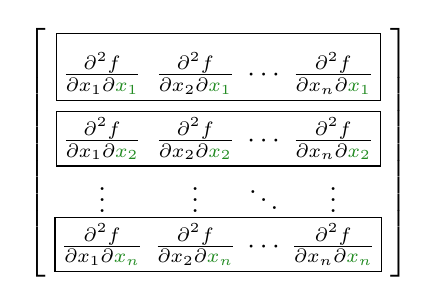
\begin{tikzpicture}[baseline=(current bounding box.center)]
		\matrix (m) [matrix of math nodes, inner sep=2pt, left delimiter={[}, right delimiter={]}] {
			|[minimum height=1cm]| \frac{\partial^2 f}{\partial x_1 \partial \textcolor{forestgreen}{x_1}} & \frac{\partial^2 f}{\partial x_2 \partial \textcolor{forestgreen}{x_1}} & \cdots & \frac{\partial^2 f}{\partial x_n \partial \textcolor{forestgreen}{x_1}} \\
			\frac{\partial^2 f}{\partial x_1 \partial \textcolor{forestgreen}{x_2}} & \frac{\partial^2 f}{\partial x_2 \partial \textcolor{forestgreen}{x_2}} & \cdots & \frac{\partial^2 f}{\partial x_n \partial \textcolor{forestgreen}{x_2}} \\
			\vdots & \vdots & \ddots & \vdots \\
			\frac{\partial^2 f}{\partial x_1 \partial \textcolor{forestgreen}{x_n}} & \frac{\partial^2 f}{\partial x_2 \partial \textcolor{forestgreen}{x_n}} & \cdots & \frac{\partial^2 f}{\partial x_n \partial \textcolor{forestgreen}{x_n}} \\
		};
		\foreach \i in {1,2,4} {
			\draw (m-\i-1.north west) rectangle (m-\i-4.south east);
		}
	\end{tikzpicture} .
	\]
\end{itemize}

\begin{itemize}
	\item In summary, the derivative rules are listed as,
	% align automatically places the equations in math mode 
	\begin{align*}
		{\color{red} D(} \boldsymbol{a}^{\top} \boldsymbol{x} {\color{red})} 
		&= \boldsymbol{a}^{\top}, \qquad &
		\fbox{\parbox{0.36\textwidth}{\( (2) f: \mathbb{R}^{n} \rightarrow \mathbb{R}, f(\boldsymbol{x}) =  \boldsymbol{a}^{\top} \boldsymbol{x} \)}} \\
		{\color{red} D(} \boldsymbol{g}(t) {\color{red})} 
		&= \left[ \begin{array}{c} \vdots \\ g_{*}'(t) \\ \vdots \end{array} \right], \qquad &
		\fbox{\parbox{0.36\textwidth}{\( (3) \boldsymbol{g}: \mathbb{R} \rightarrow \mathbb{R}^{n}, \boldsymbol{g}(t) =  \left[ \begin{array}{c} \vdots \\ g_{*}(t) \\ \vdots \end{array} \right] \)}} \\
		{\color{red} D(} \mathbf{A} \boldsymbol{x} {\color{red})} 
		&= {\color{black} \mathbf{A}}, \qquad &
		\fbox{\parbox{0.36\textwidth}{\( (4) \boldsymbol{g}: \mathbb{R}^{n} \rightarrow \mathbb{R}^{m}, \boldsymbol{g}(\boldsymbol{x}) =  \mathbf{A} \boldsymbol{x} \)}} \\
		{\color{red} D(} \mathbf{A}(\alpha \boldsymbol{x}) {\color{red})} 
		&= {\color{black} \alpha \mathbf{A}}, \\
		\frac{\mathrm{d}}{\mathrm{d} \alpha}( {\color{black}\mathbf{A}(\alpha \boldsymbol{x})} ) &= {\color{black} \mathbf{A} \boldsymbol{x}}, \\
		{\color{blue}\nabla} \boldsymbol{a}^{\top} \boldsymbol{x} 
		&= \boldsymbol{a},  \qquad & 
		\fbox{\parbox{0.36\textwidth}{\( (2) f: \mathbb{R}^{n} \rightarrow \mathbb{R}, f(\boldsymbol{x}) =  \boldsymbol{a}^{\top} \boldsymbol{x} \)}} \\
		{\color{blue}\nabla} \mathbf{A} \boldsymbol{x} 
		&= \mathbf{A}^{\top}, \qquad & 
		\fbox{\parbox{0.36\textwidth}{\( (4) \boldsymbol{g}: \mathbb{R}^{n} \rightarrow \mathbb{R}^{m}, \boldsymbol{g}(\boldsymbol{x}) =  \mathbf{A} \boldsymbol{x} \)}} \\
		{\color{blue}\nabla} \mathbf{A}(\alpha \boldsymbol{x}) 
		&=  \alpha \mathbf{A}^{\top}. \\
	\end{align*}

	\item Note that for \underline{ \(f: \mathbb{R}^n \rightarrow \mathbb{R}\) }, we have
	\[
	{\color{blue} \nabla} f(\boldsymbol{x})={\color{red} D} f(\boldsymbol{x})^{\top}.
	\]
\end{itemize}

%------------------------------------------------------%
\subsection{Differentiation product rules}
\textbf{i)} Let \(f: \mathbb{R} \rightarrow \mathbb{R}\) and \(g: \mathbb{R} \rightarrow \mathbb{R}\) be two differentiable functions, \(x \in \mathbb{R}\),
\[ 
\begin{aligned}
	D \bigg (f(x) g(x) \bigg )
	& = f(x)  D g(x)
	+g(x)  D f(x),  \\
	\nabla \bigg (f(x) g(x) \bigg )
	& = f(x)  \nabla g(x)
	+g(x)  \nabla f(x). 
\end{aligned}
\]

\noindent
\textbf{ii)} Let \(f: \mathbb{R}^{n} \rightarrow \mathbb{R}\) and \(g: \mathbb{R}^{n} \rightarrow \mathbb{R}\) be two differentiable functions, \(\boldsymbol{x} \in \mathbb{R}^{n}\),
\[ 
\begin{aligned}
	D \bigg (f(\boldsymbol{x}) g(\boldsymbol{x}) \bigg )
	& = f(\boldsymbol{x}) \big [\begin{array}{ccc}
		&D g(\boldsymbol{x}) & \end{array} \big ] 
	+g(\boldsymbol{x}) \big [\begin{array}{ccc} & D f(\boldsymbol{x}) &
	\end{array} \big ], \\
	\nabla \bigg (f(\boldsymbol{x}) g(\boldsymbol{x}) \bigg )
	& = f(\boldsymbol{x}) \left [\begin{array}{c}
		\\ \nabla g(\boldsymbol{x}) \\  \\ \end{array} \right ] 
	+g(\boldsymbol{x}) \left [\begin{array}{c} \\ \nabla f(\boldsymbol{x}) \\ \\
	\end{array} \right ].
\end{aligned}
\]

\noindent
\textbf{iii)} Let \( \boldsymbol{f}: \mathbb{R}^{n} \rightarrow \mathbb{R}^{m}\) and \( \boldsymbol{g}: \mathbb{R}^{n} \rightarrow \mathbb{R}^{m}\) be two differentiable functions, \(\boldsymbol{x} \in \mathbb{R}^{n}\),
\[ 
\begin{aligned}
	D \bigg (\boldsymbol{f}(\boldsymbol{x})^{\top} \boldsymbol{g}(\boldsymbol{x}) \bigg )
	& =\boldsymbol{f}(\boldsymbol{x})^{\top} D \boldsymbol{g}(\boldsymbol{x})+\boldsymbol{g}(\boldsymbol{x})^{\top} D \boldsymbol{f}(\boldsymbol{x}), \\
	\nabla \bigg (\boldsymbol{f}(\boldsymbol{x})^{\top} \boldsymbol{g}(\boldsymbol{x}) \bigg )
	& =\boldsymbol{f}(\boldsymbol{x})^{\top} \nabla \boldsymbol{g}(\boldsymbol{x})+\boldsymbol{g}(\boldsymbol{x})^{\top} \nabla \boldsymbol{f}(\boldsymbol{x}). \\
\end{aligned}
\]

\begin{itemize}
	\item Based on the above \textbf{derivative} rule, we have
	
	\textbf{1.} Consider \(\mathbf{A} \in \mathbb{R}^{m \times n}\) be a given matrix and \(\boldsymbol{y} \in \mathbb{R}^{m}\) a given vector. Then,
	\begin{align*}
		D\left(\boldsymbol{y}^{\top} \mathbf{A} \boldsymbol{x}\right) &=
		\boldsymbol{y}^{\top} \mathbf{A}, \\
		D\left(\boldsymbol{x}^{\top} \mathbf{A} \boldsymbol{x}\right) &=
		\boldsymbol{x}^{\top}\left(\mathbf{A}+\mathbf{A}^{\top}\right).  \qquad
		\fbox{\parbox{0.1\textwidth}{ if \(m=n\) }}
	\end{align*}
	
	
	\textbf{2.} Consider \(\mathbf{A} \in \mathbb{R}^{m \times n}\) be a given matrix and \(\boldsymbol{y} \in \mathbb{R}^{n}\) a given vector. Then,
	\[ D\left(\boldsymbol{y}^{\top} \boldsymbol{x}\right)=\boldsymbol{y}^{\top}. \]
	
	\textbf{3.} Consider if \(\mathbf{Q}\) is a symmetric matrix, then
	\[
	D\left(\boldsymbol{x}^{\top} \mathbf{Q} \boldsymbol{x}\right)=2 \boldsymbol{x}^{\top} \mathbf{Q}.
	\]
	
	In particular,
	\[
	D\left(\boldsymbol{x}^{\top} \boldsymbol{x}\right)=2 \boldsymbol{x}^{\top}.
	\]
	
	\item Based on the above \textbf{gradient} rule, we have
	
	\textbf{1.} Consider \(\mathbf{A} \in \mathbb{R}^{m \times n}\) be a given matrix and \(\boldsymbol{y} \in \mathbb{R}^{m}\) a given vector. Then,
	\begin{align*}
		\nabla \left(\boldsymbol{y}^{\top} \mathbf{A} \boldsymbol{x}\right) &= \mathbf{A}^{\top} \boldsymbol{y}, \\
		\nabla  \left(\boldsymbol{x}^{\top} \mathbf{A} \boldsymbol{x}\right) &=
		\left(\mathbf{A}+\mathbf{A}^{\top}\right) \boldsymbol{x}.  \qquad
		\fbox{\parbox{0.1\textwidth}{ if \(m=n\) }}
	\end{align*}
	
	
	\textbf{2.} Consider \(\mathbf{A} \in \mathbb{R}^{m \times n}\) be a given matrix and \(\boldsymbol{y} \in \mathbb{R}^{n}\) a given vector. Then,
	\[ \nabla \left(\boldsymbol{y}^{\top} \boldsymbol{x}\right)=\boldsymbol{y}. \]
	
	\textbf{3.} Consider if \(\mathbf{Q}\) is a symmetric matrix, then
	\[
	\nabla \left(\boldsymbol{x}^{\top} \mathbf{Q} \boldsymbol{x}\right)=2  \mathbf{Q} \boldsymbol{x}.
	\]
	
	In particular,
	\[
	\nabla \left(\boldsymbol{x}^{\top} \boldsymbol{x}\right)=2 \boldsymbol{x}.
	\]
	
\end{itemize}

%------------------------------------------------------%
\subsection{Examples}
%------------------------------------------------------%
Example 1: For the function

\begin{equation*}
	f(\boldsymbol{x})=\boldsymbol{x}^{\top} \boldsymbol{Q} \boldsymbol{x}=\boldsymbol{x}^{\top}\left[\begin{array}{cccc}
		1 & 0 & 0 & 8 \\
		8 & 0 & 1 & 0 \\
		0 & 1 & 0 & 5 \\
		8 & 0 & 3 & 1
	\end{array}\right] \boldsymbol{x}
\end{equation*}

find \(D f(\boldsymbol{x})\) and \(F(\boldsymbol{x})\).

\noindent
\textbf{Short answer:}

\begin{equation*}
	\begin{aligned}
		f(\boldsymbol{x}) & =\frac{1}{2} \boldsymbol{x}^{\top}\left(\boldsymbol{Q}+\boldsymbol{Q}^{\top}\right)\boldsymbol{x} \\
		& =\frac{1}{2} \boldsymbol{x}^{\top}\left[\begin{array}{cccc}
			2 & 8 & 0 & 16 \\
			8 & 0 & 2 & 0 \\
			0 & 2 & 0 & 8 \\
			16 & 0 & 8 & 2
		\end{array}\right] \boldsymbol{x} \\
		& = \frac{1}{2} \boldsymbol{x}^{\top} \tilde{\boldsymbol{Q}} \boldsymbol{x} .
	\end{aligned}
\end{equation*}

Therefore, \(D f(\boldsymbol{x})=\boldsymbol{x}^{\top} \tilde{\boldsymbol{Q}}\), and \(F(\boldsymbol{x})=\tilde{\boldsymbol{Q}}\).

%------------------------------------------------------%
\bigskip
\noindent
Example 2: Find \(D f(\boldsymbol{x})\) of \(f(\boldsymbol{x})=\boldsymbol{x}^{\top}\left[\begin{array}{ll}1 & 5 \\ 2 & 3\end{array}\right] \boldsymbol{x}-\boldsymbol{x}^{\top}\left[\begin{array}{c}-2 \\ 3\end{array}\right]+\pi\); Find the Hessian of \(f(\boldsymbol{x})=\frac{1}{2} \boldsymbol{x}^{\top}\left[\begin{array}{ll}2 & 3 \\ 7 & 1\end{array}\right] \boldsymbol{x}-\boldsymbol{x}^{\top}\left[\begin{array}{c}1 \\ -3\end{array}\right]+\log 3\).

\noindent
\textbf{Short answer:}

(1) \(f(\boldsymbol{x})=\frac{1}{2} \boldsymbol{x}^{\top}\left[\begin{array}{ll}2 & 7 \\ 7 & 6\end{array}\right] \boldsymbol{x}-\left[\begin{array}{ll}-2 & 3\end{array}\right] \boldsymbol{x}+\pi\). Therefore,

\begin{equation*}
	\begin{aligned}
		D f(\boldsymbol{x}) & =\boldsymbol{x}^{\top}\left[\begin{array}{ll}
			2 & 7 \\
			7 & 6
		\end{array}\right]-\left[\begin{array}{ll}
			-2 & 3
		\end{array}\right] \\
		& =\left[2 \boldsymbol{x}_{1}+7 \boldsymbol{x}_{2}+2 \quad 7 \boldsymbol{x}_{1}+6 \boldsymbol{x}_{2}-3\right] .
	\end{aligned}
\end{equation*}

(2) \(F(\boldsymbol{x})=\left[\begin{array}{ll}2 & 5 \\ 5 & 1\end{array}\right]\)

%------------------------------------------------------%
\bigskip
\noindent
Example 3: For the function \(f=f\left(x_{1}, x_{2}\right)=x_{1}^{2} x_{2}+x_{2}^{3} x_{1}\),

(1) find the gradient of \(f\) at \(\boldsymbol{x}=\left[\begin{array}{ll}2 & 1\end{array}\right]^{\top}\);

(2) find the rate of increase of \(f\) at the point \(\boldsymbol{x}=\left[\begin{array}{ll}2 & 1\end{array}\right]^{\top}\) in the direction \(\boldsymbol{d}=\left[\begin{array}{ll}4 & 3\end{array}\right]^{\top}\).

\noindent
\textbf{Short answer:}
(1) \(\nabla f(\boldsymbol{x})=\left[\begin{array}{l}\frac{\partial f}{\partial x_{1}} \\ \frac{\partial f}{\partial x_{2}}\end{array}\right]=\left[\begin{array}{l}2 x_{1} x_{2}+x_{2}^{3} \\ x_{1}^{2}+3 x_{1} x_{2}^{2}\end{array}\right], \nabla f(\left[\begin{array}{c}2 \\ 1\end{array}\right])=\left[\begin{array}{c}5 \\ 10\end{array}\right]\).

(2) \(\frac{\boldsymbol{d}^{\top}}{\|\boldsymbol{d}\|} \nabla f(\boldsymbol{x})=10\).


%------------------------------------------------------%
\bigskip
\noindent
Example 4: Consider the function

\begin{equation*}
	f(\boldsymbol{x})=\left(\boldsymbol{a}^{\top} \boldsymbol{x}\right)\left(\boldsymbol{b}^{\top} \boldsymbol{x}\right),
\end{equation*}

where \(\boldsymbol{a}, \boldsymbol{b}\), and \(\boldsymbol{x}\) are \(n\)-dimensional vectors.

(1) Find \(\nabla f(\boldsymbol{x})\).

(2) Find the Hessian \(F(\boldsymbol{x})\).

\noindent
\textbf{Short answer:}
(1) We have

\begin{equation*}
	f(\boldsymbol{x})=\left(\boldsymbol{a}^{\top} \boldsymbol{x}\right)\left(\boldsymbol{b}^{\top} \boldsymbol{x}\right)=\boldsymbol{x}^{\top}\left(\boldsymbol{a} \boldsymbol{b}^{\top}\right) \boldsymbol{x}=\boldsymbol{x}^{\top} \boldsymbol{Q} \boldsymbol{x},
\end{equation*}

where \(\boldsymbol{Q} \in \mathbb{R}^{n \times n}\). Note that \(\boldsymbol{Q}\) can be non-symmetric. We then first symmetrize the quadratic form as

\begin{equation*}
	f=\frac{1}{2} \boldsymbol{x}^{\top}\left(\boldsymbol{Q}+\boldsymbol{Q}^{\top}\right) \boldsymbol{x}=\frac{1}{2} \boldsymbol{x}^{\top}\left(\boldsymbol{a} \boldsymbol{b}^{\top}+\boldsymbol{b} \boldsymbol{a}^{\top}\right) \boldsymbol{x} .
\end{equation*}

Therefore,

\begin{equation*}
	\nabla f(\boldsymbol{x})=\left(\boldsymbol{a} \boldsymbol{b}^{\top}+\boldsymbol{b} \boldsymbol{a}^{\top}\right) \boldsymbol{x}
\end{equation*}

(2) \(F(x)=\boldsymbol{a} \boldsymbol{b}^{\top}+\boldsymbol{b} \boldsymbol{a}^{\top}\).

\bigskip

\noindent
[Ref]: Edwin K.P. Chong, Stanislaw H. Żak, ``PART I MATHEMATICAL REVIEW" in ``An introduction to optimization", 4th Edition, John Wiley and Sons, Inc. 2013.

%------------------------------------------------------%
%------------------------------------------------------%
\section{Direction of Maximum Increase}
%------------------------------------------------------%
%------------------------------------------------------%

\subsection{Concept}
\begin{itemize}
	\item A vector \(\boldsymbol{d} \in \mathbb{R}^{n}, \boldsymbol{d} \neq \boldsymbol{0}\), is a feasible direction at \( \boldsymbol{x} \in \Omega\) if there exists \(\alpha_{0}>0\) such that \(\boldsymbol{x}+\alpha \boldsymbol{d} \in \Omega\) for all \( \alpha \in\left[0, \alpha_{0}\right] \).

	\item Let \(f: \mathbb{R}^{n} \rightarrow \mathbb{R}\) be a real-valued function and let \(\boldsymbol{d}\) be a feasible direction at \(\boldsymbol{x} \in \Omega \). The directional derivative of \(f\) in the direction \(\boldsymbol{d}\), denoted \(\partial f / \partial \boldsymbol{d}\) is the real-valued function defined by
	
	\[
	\frac{\partial f}{\partial \boldsymbol{d}}(\boldsymbol{x})=\lim _{\alpha \rightarrow 0} \frac{f(\boldsymbol{x}+\alpha \boldsymbol{d})-f(x)}{\alpha} = \boldsymbol{d}^{\top} \nabla f(\boldsymbol{x})
	= \sum_{i=1}^{n} \frac{\partial f(\boldsymbol{x})}{x_i} d_i
	\]

	\item If Euclidean norm \(\|\boldsymbol{d}\|_2=1\), then \(\partial f / \partial \boldsymbol{d}\) is the \underline{rate of increase} of \(f\) at \(\boldsymbol{x}\) in the direction \(\boldsymbol{d}\).
	
	\[\frac{\partial f}{\partial \boldsymbol{d}}(\boldsymbol{x})=\left.\frac{d}{d \alpha} f(\boldsymbol{x}+\alpha \boldsymbol{d})\right|_{\alpha=0}=\nabla f(\boldsymbol{x})^{\top} \boldsymbol{d}=\langle\nabla f(\boldsymbol{x}), \boldsymbol{d}\rangle=\boldsymbol{d}^{\top} \nabla f(\boldsymbol{x}) \]

	\item If Euclidean norm \(\|\boldsymbol{d}\|_2 \neq 1\), the rate of increase of \(f\) at \(\boldsymbol{x}\) in the direction \(\boldsymbol{d}\), normalize \(\boldsymbol{d}\), replace \(\boldsymbol{d}\) with \(\frac{\boldsymbol{d}}{\|\boldsymbol{d}\|_2}\), that is, \(\frac{\boldsymbol{d}^{\top}}{\|\boldsymbol{d}\|_2} \nabla f(\boldsymbol{x}) \).
	
	\[ \left\| \frac{\boldsymbol{d}}{\|\boldsymbol{d}\|} \right\| 
	= \left\| \frac{1}{\|\boldsymbol{d}\|}  \left[ \begin{array}{c} \\ \boldsymbol{d} \\ \\ \end{array} \right]\right \|
	= \frac{1}{\|\boldsymbol{d}\|}  \|\boldsymbol{d}\|
	= 1 \]
\end{itemize}

%------------------------------------------------------%
\subsection{Practice problems}
\begin{enumerate}
	\item Given the following function,
\end{enumerate}

\begin{equation*}
	f\left(x_{1}, x_{2}\right)=x_{1}^{2} x_{2}+x_{2}^{3} x_{1} .
\end{equation*}

(1) In what direction does the function \(f\) increase most rapidly at the point \(\boldsymbol{x}^{(0)}=\left[\begin{array}{ll}2 & 1\end{array}\right]^{\top}\) ?

(2) What is the rate of increase of \(f\) at the point \(\boldsymbol{x}^{(0)}\) in the direction of maximum increase of \(f\) ?

(3) Find the rate of increase of \(f\) at the point \(\boldsymbol{x}^{(0)}\) in the direction \(\boldsymbol{d}=\left[\begin{array}{ll}4 & 3\end{array}\right]^{\top}\).

\textbf{Short answer:}
(1) A differentiable function \(f\) increases most rapidly in the direction of the gradient. In this problem, we have

\begin{equation*}
	\nabla f(\boldsymbol{x})=\left[\begin{array}{l}
		2 x_{1} x_{2}+x_{2}^{3} \\
		x_{1}^{2}+3 x_{1} x_{2}^{2}
	\end{array}\right] .
\end{equation*}

Hence,

\begin{equation*}
	\nabla f\left(\boldsymbol{x}^{(0)}\right)=\left[\begin{array}{c}
		5 \\
		10
	\end{array}\right]
\end{equation*}

(2) The rate of increase of \(f\) at \(\boldsymbol{x}^{(0)}\) in the direction \(\nabla f\left(\boldsymbol{x}^{(0)}\right)\) is

\begin{equation*}
	\nabla f\left(\boldsymbol{x}^{(0)}\right)^{\top} \frac{\nabla f\left(\boldsymbol{x}^{(0)}\right)}{\left\|\nabla f\left(\boldsymbol{x}^{(0)}\right)\right\|}=\left\|\nabla f\left(\boldsymbol{x}^{(0)}\right)\right\|=5 \sqrt{5} .
\end{equation*}

(3) The rate of increase of \(f\) at \(\boldsymbol{x}^{(0)}\) in the direction \(\boldsymbol{d}\) is

\begin{equation*}
	\nabla f\left(\boldsymbol{x}^{(0)}\right)^{\top} \frac{\boldsymbol{d}}{\|\boldsymbol{d}\|}=\left[\begin{array}{ll}
		5 & 10
	\end{array}\right]\left[\begin{array}{l}
		4 \\
		3
	\end{array}\right] \frac{1}{5}=10 .
\end{equation*}

%------------------------------------------------------%
\bigskip
\noindent
\begin{enumerate}
	\setcounter{enumi}{1}
	\item Find the range of values of the parameter \(a\) for which \(\boldsymbol{d}=\left[\begin{array}{ll}a & 1\end{array}\right]^{\top}\) is a direction of ascent of
\end{enumerate}

\begin{equation*}
	f=f\left(x_{1}, x_{2}\right)=x_{1}^{3}+x_{1} x_{2}-x_{1}^{2} x_{2}^{2},
\end{equation*}

at the point \(\boldsymbol{x}^{(0)}=\left[\begin{array}{ll}1 & 1\end{array}\right]^{\top}\).


\textbf{Short answer:}
For the direction of ascent, we have \(\boldsymbol{d}^{\top} \nabla f>0\). We first calculate the gradient

\begin{equation*}
	\nabla f(\boldsymbol{x})=\left[\begin{array}{c}
		3 x_{1}^{2}+x_{2}-2 x_{1} x_{2}^{2} \\
		x_{1}-2 x_{1}^{2} x_{2}
	\end{array}\right] .
\end{equation*}

Hence,

\begin{equation*}
	\nabla f\left(\boldsymbol{x}^{(0)}\right)=\left[\begin{array}{c}
		2 \\
		-1
	\end{array}\right]
\end{equation*}

We then need

\begin{equation*}
	\boldsymbol{d}^{\top} \nabla f\left(\boldsymbol{x}^{(0)}\right)=\left[\begin{array}{ll}
		a & 1
	\end{array}\right]\left[\begin{array}{c}
		2 \\
		-1
	\end{array}\right]=2 a-1>0 .
\end{equation*}

We have \(a>\frac{1}{2}\).

\include{./sections/p1_definiteness}
%------------------------------------------------------%
%------------------------------------------------------%
\section{Taylor Series Expansion}
%------------------------------------------------------%
%------------------------------------------------------%

%------------------------------------------------------%
\subsection{Concept}
\begin{itemize}
	\item Suppose \(f \in \mathcal{C}^{2}\). The Taylor series expansion of a real-valued function \(f\) : \(\mathbb{R}^{n} \rightarrow \mathbb{R}\) about the point \(\boldsymbol{x}_{0} \in \mathbb{R}^{n}\) is
\end{itemize}

\begin{equation*}
	\begin{aligned}
		f(\boldsymbol{x})=f\left(\boldsymbol{x}_{0}\right) 
		& + \left[ \begin{array}{ccc}
			& D f\left(\boldsymbol{x}_{0}\right) & \\
			\end{array}
			\right]
			\left[ \begin{array}{c} 
				 \\ \left(\boldsymbol{x}-\boldsymbol{x}_{0}\right) \\ \\
			\end{array}
			\right] \\
		& +\frac{1}{2}
			\left[ \begin{array}{ccc} 
				& \left(\boldsymbol{x}-\boldsymbol{x}_{0}\right)^{\top}  & \\
			\end{array}
			\right]
			\left[ \begin{array}{ccc}
				& & \\
				& D^2 f\left(\boldsymbol{x}_{0}\right) & \\
				& & \\
			\end{array}
			\right]
			\left[ \begin{array}{c} 
				\\ \left(\boldsymbol{x}-\boldsymbol{x}_{0}\right) \\ \\
			\end{array}
			\right]
			+o\left(\left\|\boldsymbol{x}-\boldsymbol{x}_{0}\right\|^{2}\right) .
	\end{aligned}
\end{equation*}

\begin{itemize}
	\item The linear approximation of \(f\) about the point \(\boldsymbol{x}_{0}\) is
\end{itemize}

\begin{equation*}
	l(\boldsymbol{x})=f\left(\boldsymbol{x}_{0}\right)+D f\left(\boldsymbol{x}_{0}\right)\left(\boldsymbol{x}-\boldsymbol{x}_{0}\right) .
\end{equation*}

\begin{itemize}
	\item The quadratic approximation of \(f\) about the point \(\boldsymbol{x}_{0}\) is
\end{itemize}

\begin{equation*}
	q(\boldsymbol{x})=f\left(\boldsymbol{x}_{0}\right)+D f\left(\boldsymbol{x}_{0}\right)\left(\boldsymbol{x}-\boldsymbol{x}_{0}\right)+\frac{1}{2}\left(\boldsymbol{x}-\boldsymbol{x}_{0}\right)^{\top} D^{2} f\left(\boldsymbol{x}_{0}\right)\left(\boldsymbol{x}-\boldsymbol{x}_{0}\right) .
\end{equation*}

%------------------------------------------------------%
\subsection{Examples}

\begin{enumerate}
	\item Compute the linear \(l\left(x_{1}, x_{2}\right)\) and quadratic \(q\left(x_{1}, x_{2}\right)\) approximations of the function \(f\left(x_{1}, x_{2}\right)=x_{1}+\frac{3 x_{2}}{x_{1}}\), at the point \(\boldsymbol{x}^{(0)}=\left[\begin{array}{ll}1 & 2\end{array}\right]^{\top}\).
\end{enumerate}

\textbf{Short answer:}

(1) \[l(\boldsymbol{x})=f\left(\boldsymbol{x}^{(0)}\right)+D f\left(\boldsymbol{x}^{(0)}\right)\left(\boldsymbol{x}-\boldsymbol{x}^{(0)}\right),\]

\begin{equation*}
	D f(\boldsymbol{x}^{(0)})
	=\left[\begin{array}{ll}
		\frac{\partial f}{\partial x_{1}} & \frac{\partial f}{\partial x_{2}}
		\end{array}
		\right]
	=\left[\begin{array}{ll}
		1-\frac{3 x_{2}}{x_{1}^{2}} & \frac{3}{x_{1}}
		\end{array}
		\right]
	=\left[\begin{array}{ll}
		-5 & 3
	\end{array}\right].
\end{equation*}

Therefore,

\begin{equation*}
	l(\boldsymbol{x})=7+\left[\begin{array}{ll}
		-5 & 3
	\end{array}\right]\left[\begin{array}{l}
		x_{1}-1 \\
		x_{2}-2
	\end{array}\right]=-5 x_{1}+3 x_{2}+6 .
\end{equation*}

(2)
\[q(\boldsymbol{x})=l(\boldsymbol{x})+\frac{1}{2}\left(\boldsymbol{x}-\boldsymbol{x}_{0}\right)^{\top} D^{2} f\left(\boldsymbol{x}_{0}\right)\left(\boldsymbol{x}-\boldsymbol{x}_{0}\right). \]

\begin{equation*}
	F(\boldsymbol{x}^{(0)})
	=D^{2} f(\boldsymbol{x})
	=\left[\begin{array}{cc}
		\frac{6 x_{2}}{x_{1}^{3}} & -\frac{3}{x_{1}^{2}} \\
		-\frac{3}{x_{1}^{2}} & 0
	\end{array} 
	\right]
	= \left[\begin{array}{cc}12 & -3 \\ -3 & 0\end{array}\right].
\end{equation*}

Therefore,

\begin{equation*}
	\begin{aligned}
		q(\boldsymbol{x}) & =l(\boldsymbol{x})+\frac{1}{2}\left[\begin{array}{ll}
			x_{1}-1 & x_{2}-2
		\end{array}\right]\left[\begin{array}{cc}
			12 & -3 \\
			-3 & 0
		\end{array}\right]\left[\begin{array}{l}
			x_{1}-1 \\
			x_{2}-2
		\end{array}\right] \\
		& =6 x_{1}^{2}-3 x_{1} x_{2}-11 x_{1}+6 x_{2}+6 .
	\end{aligned}
\end{equation*}


%------------------------------------------------------%
\bigskip
\noindent
\begin{enumerate}
	\setcounter{enumi}{1}
	\item Perform a second-order Taylor series expansion of the function
	
	\begin{equation*}
		f=f\left(x_{1}, x_{2}\right)=3 x_{1}^{2}x_{2}+x_{1} x_{2}^{4}-5 x_{1}+7,
	\end{equation*}
	
	at the point \(\boldsymbol{x}^{(0)}=\left[\begin{array}{ll}0 & 1\end{array}\right]^{\top}\).
\end{enumerate}
	
\textbf{Short answer:}

\begin{equation*}
	\begin{aligned}
		f(\boldsymbol{x}) & =f\left(\boldsymbol{x}_{0}\right)+D f\left(\boldsymbol{x}_{0}\right)\left(\boldsymbol{x}-\boldsymbol{x}_{0}\right) \\
		 	  & \hspace{1.6cm} +\frac{1}{2}\left(\boldsymbol{x}-\boldsymbol{x}_{0}\right)^{\top} 
		 	  	D^{2} f\left(\boldsymbol{x}_{0}\right)\left(\boldsymbol{x}-\boldsymbol{x}_{0}\right)+o\left(\left\|\boldsymbol{x}-\boldsymbol{x}_{0}\right\|^{2}\right) . \\
		Df(\boldsymbol{x}) & =\nabla f(\boldsymbol{x})^{\top}
			= \left[\begin{array}{c}
			6 x_{1} x_{2}+x_{2}^{4}-5 \\
			3 x_{1}^{2}+4 x_{1} x_{2}^{3}
			\end{array}\right]^{\top} . \\
		F(\boldsymbol{x}) & =D^{2} f(\boldsymbol{x})=
			\left[\begin{array}{cc}
			6 x_{2} & 6 x_{1}+4 x_{2}^{3} \\
			6 x_{1}+4 x_{2}^{3} & 12 x_{1} x_{2}^{2}
			\end{array}\right] .
	\end{aligned}
\end{equation*}

We have \(D f\left(\boldsymbol{x}^{(0)}\right)=\left[\begin{array}{ll}-4 & 0\end{array}\right]\), and \(F\left(\boldsymbol{x}^{(0)}\right)=\left[\begin{array}{ll}6 & 4 \\ 4 & 0\end{array}\right]\). Therefore,

\begin{equation*}
	\begin{aligned}
	q(\boldsymbol{x})
		  & = 3(0)^{2}(1)+(0)(1)^{4}-5(0)+7 
		  		+ \left[\begin{array}{cc} -4 & 0 \\ \end{array}\right] 
		  		\left[\begin{array}{c} x_{1}-0 \\ x_{2}-1 \end{array}\right]\\
		  &	\qquad +  \frac{1}{2} \left[\begin{array}{c} x_{1}-0 \\ x_{2}-1 \end{array}\right]^{\top}
		  		\left[\begin{array}{ll}6 & 4 \\ 4 & 0\end{array}\right]
		  		\left[\begin{array}{c} x_{1}-0 \\ x_{2}-1 \end{array}\right] \\
		  & = 7 - 4x_{1} + \left[\begin{array}{cccc} 3x_{1}+2x_{2} -2 & & 2x_{1} \end{array}\right]
		  		\left[\begin{array}{c} x_{1}-0 \\ x_{2}-1 \end{array}\right] \\
		  & =3 x_{1}^{2}+4 x_{1} x_{2}-8 x_{1}+7. \\
		 f(\boldsymbol{x})
		 & =q(\boldsymbol{x})+o\left(\left\|\boldsymbol{x}-\boldsymbol{x}_{0}\right\|^{2}\right) \\
		 & =3 x_{1}^{2}+4 x_{1} x_{2}-8 x_{1}+7 +o\left(\left\|\boldsymbol{x}-\boldsymbol{x}_{0}\right\|^{2}\right).
	\end{aligned}
\end{equation*}

\bigskip

\noindent
[Ref]: Edwin K.P. Chong, Stanislaw H. Żak, ``PART I MATHEMATICAL REVIEW" in ``An introduction to optimization", 4th Edition, John Wiley and Sons, Inc. 2013.

%------------------------------------------------------%
%------------------------------------------------------%
\section{Convex set}
%------------------------------------------------------%
%------------------------------------------------------%

%------------------------------------------------------%
\subsection{Concept}


\medskip

%------------------------------------------------------%
\subsection{Examples}
\noindent
%------------------------------------------------------%

\noindent
\begin{enumerate}
	
	\item Show that the set \(\left\{\boldsymbol{x} \in \mathbb{R}^{n}:\|\boldsymbol{x}\| \leq r\right\}\) is convex, where \(r>0\) is a given real number and \(\|\boldsymbol{x}\|=\sqrt{\boldsymbol{x}^{\top} \boldsymbol{x}}\) is the Euclidean norm of \(\boldsymbol{x} \in \mathbb{R}^{n} \).
	
\end{enumerate}


\textbf{Short answer:}

To show that the set \(S = \{\boldsymbol{x} \in \mathbb{R}^{n} : \|\boldsymbol{x}\| \leq r\}\) is convex, where \(r>0\) is a given real number and \(\|\boldsymbol{x}\|=\sqrt{\boldsymbol{x}^{\top} \boldsymbol{x}}\) is the Euclidean norm of \(\boldsymbol{x} \in \mathbb{R}^{n}\), we need to demonstrate that for any two points \(\boldsymbol{x}, \boldsymbol{y} \in S\) and any \(\lambda \in [0, 1]\), the point \(\lambda \boldsymbol{x} + (1-\lambda) \boldsymbol{y}\) also belongs to \(S\), i.e., \[ \|\lambda \boldsymbol{x} + (1-\lambda) \boldsymbol{y}\| \leq r. \] Given \(\boldsymbol{x}, \boldsymbol{y} \in S\), it implies \(\|\boldsymbol{x}\| \leq r\) and \(\|\boldsymbol{y}\| \leq r\). For any \(\lambda \in [0, 1]\), consider: \[ \|\lambda \boldsymbol{x} + (1-\lambda) \boldsymbol{y}\|^2 = \lambda^2 \|\boldsymbol{x}\|^2 + 2\lambda(1-\lambda) \boldsymbol{x}^{\top}\boldsymbol{y} + (1-\lambda)^2 \|\boldsymbol{y}\|^2. \] By applying the Cauchy-Schwarz inequality, \(\boldsymbol{x}^{\top}\boldsymbol{y} \leq \|\boldsymbol{x}\|\|\boldsymbol{y}\|\), we have: \[ \|\lambda \boldsymbol{x} + (1-\lambda) \boldsymbol{y}\|^2 \leq \lambda^2 r^2 + 2\lambda(1-\lambda) r^2 + (1-\lambda)^2 r^2 = r^2. \] Hence, taking the square root on both sides, we obtain \(\|\lambda \boldsymbol{x} + (1-\lambda) \boldsymbol{y}\| \leq r\), proving the convexity of \(S\). 

%------------------------------------------------------%
\medskip
\noindent
\begin{enumerate}
	\setcounter{enumi}{1}
	
	\item Prove
	(a) let \( \boldsymbol{A}\) be an \(m \times n\) matrix, \( \boldsymbol{b} \in \mathbb{R}^m\), and let \(S=\left\{ \boldsymbol{x} \in \mathbb{R}^n:  \boldsymbol{A}  \boldsymbol{x}= \boldsymbol{x}\right\}\). Then the set \(S\) is a convex subset of \(\mathbb{R}^n\).
	(b) In \(\mathbb{R}^n\) the set \(H=\left\{ \boldsymbol{x} \in \mathbb{R}^n: a_1 x_1+\ldots+a_n x_n=c\right\}\) is a convex set. For any particular choice of constants \(a_i\) it is a hyperplane in \(\mathbb{R}^n\).
	
\end{enumerate}


\textbf{Short answer:}

(a) Let \( \boldsymbol{x}^{(1)},  \boldsymbol{x}^{(2)} \in S\). Then
\[
 \boldsymbol{A}\left((1-\lambda)  \boldsymbol{x}^{(1)}+\lambda  \boldsymbol{x}^{(2)}\right)=(1-\lambda)  \boldsymbol{A}\left( \boldsymbol{x}^{(1)}\right)+\lambda  \boldsymbol{A}\left( \boldsymbol{x}^{(2)}\right)=(1-\lambda)  \boldsymbol{b}+\lambda  \boldsymbol{b}= \boldsymbol{b} .
\]

(b) Just take \( \boldsymbol{A}=\left(a_1, \ldots, a_n\right)\) in (a).



%------------------------------------------------------%
\medskip
\noindent
\begin{enumerate}
	\setcounter{enumi}{2}
	
	\item Prove that the intersection of any number of convex sets is convex.
	
\end{enumerate}


\textbf{Short answer:}

Let \(\left\{K_\alpha\right\}_{\alpha \in A}\) be a family of convex sets, and let \(\mathcal{K}:=\cap_{\alpha \in A} K_\alpha\). Then, for any \(x, y \in \mathcal{K}\) by definition of the intersection of a family of sets, \(x, y \in K_\alpha\) for all \(\alpha \in A\) and each of these sets is convex. Hence for any \(\alpha \in A\), and \(\lambda \in[0,1],(1-\lambda) x+\lambda y \in K_\alpha\). Hence \((1-\lambda) x+\lambda y \in \mathcal{K}\).



%------------------------------------------------------%
\medskip
\noindent
\begin{enumerate}
	\setcounter{enumi}{3}
	
	\item Let \(f_1, f_2, \ldots, f_k\) be convex functions and \(w_1, w_2, \ldots, w_k\) be nonnegative real numbers. Prove that \(f(x)=\sum_{i=1}^k w_i f_i(x)\) is a convex function.
	
\end{enumerate}


\textbf{Short answer:}

For any \(i=1, \ldots, k\), any \(x, y \in \operatorname{dom} f_i\), and \(\lambda \in[0,1]\), we have
\[
f_i(\lambda x+(1-\lambda) y) \leq \lambda f_i(x)+(1-\lambda) f_i(y)
\]

Then it follows that
\[
f(\lambda x+(1-\lambda) y)=\sum_{i=1}^k w_i f_i(\lambda x+(1-\lambda) y) \leq \sum_{i=1}^k w_i\left(\lambda f_i(x)+(1-\lambda) f_i(y)\right)=\lambda f(x)+(1-\lambda) f(y)
\]

Hence, \(f(x)\) is convex.

%------------------------------------------------------%
\medskip
\noindent
\begin{enumerate}
	\setcounter{enumi}{4}
	
	\item (a) Prove that \(|x|^\alpha\) is convex on \(\mathbb{R}\) for \(\alpha \geq 1\).
	(b) Prove that if \(f_1, f_2: \mathbb{R}^N \rightarrow \mathbb{R}\) are convex, then \(\max \left(f_1, f_2\right)\) is convex.
	
\end{enumerate}


\textbf{Short answer:}

(a) When \(\alpha=1\), we can directly verify the convexity of \(|x|\) by definition. When \(\alpha>1, f(x)=x^\alpha\) is twice-differentiable and \(f^{\prime \prime}(x)=\alpha(\alpha-1) x^{\alpha-2} \geq 0\). Then the result follows from second-order condition.
(b) Let \(f=\max \left(f_1, f_2\right)\). Since \(\forall x, y \in \mathbb{R}^N, \lambda \in[0,1]\), we have
\[
f_i(\lambda x+(1-\lambda) y) \leq \lambda f_i(x)+(1-\lambda) f_i(y) \leq \lambda f(x)+(1-\lambda) f(y), i=1,2 .
\]

Therefore,
\[
f(\lambda x+(1-\lambda) y)=\max \left(f_1(\lambda x+(1-\lambda) y), f_2(\lambda x+(1-\lambda) y) \leq \lambda f(x)+(1-\lambda) f(y)\right.
\]


%------------------------------------------------------%
\medskip
\noindent
\begin{enumerate}
	\setcounter{enumi}{5}
	
	\item (a) Prove that the Quadratic-Over-Linear function \(f\left(x_1, x_2\right)=\frac{x_1^2}{x_2}\) is convex on \(\mathbb{R} \times(0, \infty)\).
	(b) Prove that the quadratic function
	\[
	f(\boldsymbol{x})=\frac{1}{2} \boldsymbol{x}^{\mathrm{T}} \boldsymbol{P} \boldsymbol{x}+\boldsymbol{q}^{\mathrm{T}} \boldsymbol{x}+r,
	\]
	where \(\boldsymbol{P}\) is symmetric, is convex if and only if \(\boldsymbol{P}\) is positive semi-definite.
	
\end{enumerate}


\textbf{Short answer:}

(a) We have
\[
\nabla^2 f=\left(\begin{array}{cc}
	\frac{2}{x_2} & \frac{-2 x_1}{x_2^2} \\
	\frac{-2 x_1}{x_2^2} & \frac{2 x_1^2}{x^3}
\end{array}\right)=\frac{2}{x_2^3}\left(\begin{array}{cc}
	x_2^2 & -x_1 x_2 \\
	-x_1 x_2 & x_1^2
\end{array}\right) .
\]

Since \(\nabla^2 f \succeq 0, \forall\left(x_1, x_2\right) \in \mathbb{R} \times(0, \infty), f\left(x_1, x_2\right)\) is convex on \(\mathbb{R} \times(0, \infty)\).
(b) Just note that the Hessian of \(f\) is
\[
\nabla^2 f=\left(\frac{\partial^2 f(\boldsymbol{x})}{\partial x_i \partial x_j}\right)_{1 \leq i, j \leq N}= \boldsymbol{P}
\]
and use second-order condition.




% Part 2: Unconstrained Optimization
%------------------------------------------------------%
%------------------------------------------------------%
\section{FONC, SONC and SOSC}
%------------------------------------------------------%
%------------------------------------------------------%

%------------------------------------------------------%
\subsection{Concept}

\begin{itemize}
	\item \(\mathscr{THEOREM}\)6.1 (\textbf{FONC}) Let \(\Omega\) be a subset of \(\mathbb{R}^{n}\) and \(f \in \mathcal{C}^{1}\) a real-valued function on \(\Omega\). If \(\boldsymbol{x}^{*}\) is a local minimizer of \(f\) over \(\Omega\), then for any feasible direction \(\boldsymbol{d}\) at \(\boldsymbol{x}^{*}\), we have
	
	\begin{equation*}
		\boldsymbol{d}^{\top} \nabla f\left(\boldsymbol{x}^{*}\right) \geq 0.
	\end{equation*}

	\item \(\mathscr{COROLLARY}\)6.1 (Interior Case \textbf{FONC}) Let \(\Omega\) be a subset of \(\mathbb{R}^{n}\) and \(f \in \mathcal{C}^{1}\), a real-valued function on \(\Omega\). If \(\boldsymbol{x}^{*}\) is a local minimizer of \(f\) over \(\Omega\) and if \(\boldsymbol{d}^{*}\) is an interior point of \(\Omega\), then
	
	\begin{equation*}
		\nabla f\left(\boldsymbol{x}^{*}\right)=0 .
	\end{equation*}

	\item \(\mathscr{THEOREM}\)6.2 (\textbf{SONC}) Let \(\Omega \subset \mathbb{R}^{n}, f \in \mathcal{C}^{2}\) a function on \(\Omega, \boldsymbol{x}^{*}\) a local minimizer of \(f\) over \(\Omega\), and \(\boldsymbol{d}\) a feasible direction at \(x^{*}\). If \(\boldsymbol{d}^{\top} \nabla f\left(x^{*}\right)=0\), then
	
	\begin{equation*}
		\boldsymbol{d}^{\top} \boldsymbol{F} \left(\boldsymbol{x}^{*}\right) \boldsymbol{d} \geq 0,
	\end{equation*}
	
	where \(F\) is the Hessian of \(f\).

	\item  \(\mathscr{COROLLARY}\)6.2 (Interior Case \textbf{SONC}) Let \(\boldsymbol{x}^{*}\) be an interior point of \(\Omega \subset \mathbb{R}^{n}\). If \(\boldsymbol{x}^{*}\) is a local minimizer of \(f: \Omega \rightarrow \mathbb{R}, f \in \mathcal{C}^{2}\), then
	
	\begin{equation*}
		\nabla f\left(\boldsymbol{x}^{*}\right)=0,
	\end{equation*}
	
	and \(F\left(\boldsymbol{x}^{*}\right)\) is positive semi-definite; that is, for all \(\boldsymbol{d} \in \mathbb{R}^{n}\),
	
	\begin{equation*}
		\boldsymbol{d}^{\top} \boldsymbol{F} \left(\boldsymbol{x}^{*}\right) \boldsymbol{d} \geq 0 .
	\end{equation*}

	\item \(\mathscr{THEOREM}\)6.3 (Interior Case \textbf{SOSC}) Let \(f \in \mathcal{C}^{2}\) be defined on a region in which \(\boldsymbol{x}^{*}\) is an interior point. Suppose that
	
	\begin{enumerate}
		\item \(\nabla f\left(\boldsymbol{x}^{*}\right)=0\),
		
		\item \(\boldsymbol{F} \left(\boldsymbol{x}^{*}\right) \succ 0\).
		
	\end{enumerate}
	
	Then, \(\boldsymbol{x}^{*}\) is a strict local minimizer of \(f\).
	
	\item (Recall) A vector \(\boldsymbol{d} \in \mathbb{R}^{n}, \boldsymbol{d} \neq \boldsymbol{0}\), is a feasible direction at \(\boldsymbol{x} \in \Omega\) if there exists \(\alpha_{0}>0\) such that \(\boldsymbol{x}+\alpha \boldsymbol{d}  \in \Omega\) for all \(\alpha \in\left[0, \alpha_{0}\right]\).

\end{itemize}

%------------------------------------------------------%
\subsection{Examples}

\noindent
\begin{enumerate}
	\item Does the function

	\begin{equation*}
		f(\boldsymbol{x})=\boldsymbol{x}^{\top}\left[\begin{array}{cc}
			-2 & 2 \\
			0 & -1
		\end{array}\right] \boldsymbol{x}+\boldsymbol{x}^{\top}\left[\begin{array}{c}
			1 \\
			-1
		\end{array}\right]
	\end{equation*}
	
	where \(\boldsymbol{x} \in \mathbb{R}^{2}\), have a minimizer or a maximizer? If it does, then find it; otherwise explain why it does not.
\end{enumerate}

\textbf{Short answer:}

For an unconstrained optimization problem, if a point is a maximizer or a miminizer, then it satisfies the FONC, that is \(\nabla f(\boldsymbol{x})=0\). We calculate the gradient of \(f\) as follows:

\begin{equation*}
	f(\boldsymbol{x})=\boldsymbol{x}^{\top} \boldsymbol{Q} \boldsymbol{x}+\boldsymbol{x}^{\top} \boldsymbol{b}=\frac{1}{2} \boldsymbol{x}^{\top}\left(\boldsymbol{Q}+\boldsymbol{Q}^{\top}\right) \boldsymbol{x}+\boldsymbol{x}^{\top} \boldsymbol{b} .
\end{equation*}

Then

\begin{equation*}
	\nabla f(\boldsymbol{x})=\left(\boldsymbol{Q}+\boldsymbol{Q}^{\top}\right) \boldsymbol{x}+\boldsymbol{b}.
\end{equation*}

Let \(\nabla f(\boldsymbol{x})=0\), we have

\begin{equation*}
	\left[\begin{array}{cc}
		-4 & 2 \\
		2 & -2
	\end{array}\right] \boldsymbol{x}=\left[\begin{array}{c}
		-1 \\
		1
	\end{array}\right].
\end{equation*}

Hence

\begin{equation*}
	\boldsymbol{x}^{*}=\left[\begin{array}{c}
		0 \\
		-0.5
	\end{array}\right] .
\end{equation*}

\(F(\boldsymbol{x})\) is n.d. since \(-F(\boldsymbol{x})\) is p.d. \(\Rightarrow \boldsymbol{x}^{*}\) is a maximizer.

%------------------------------------------------------%
\medskip
\noindent
\begin{enumerate}
	\setcounter{enumi}{1}
	\item 
	(1) Does the function: \(f\left(x_{1}, x_{2}\right)=x_{1}^{2}+2 x_{1} x_{2}+x_{2}^{2}-x_{1}+x_{2}+5\) have a minimizer or a maximizer? If it does, then find it; otherwise explain why it does not. (2) Does the function: \(f\left(x_{1}, x_{2}\right)=x_{1} x_{2}-2 x_{1}^{2}-x_{2}^{2}-x_{1}-x_{2}+5\) have a minimizer or a maximizer? If it does, then find it, otherwise explain why it does not.
	
\end{enumerate}


\textbf{Short answer:}

(1) \(\nabla f(\boldsymbol{x})=\left[\begin{array}{l}2 x_{1}+2 x_{2}-1 \\ 2 x_{1}+2 x_{2}+1\end{array}\right]=\left[\begin{array}{l}0 \\ 0\end{array}\right] \Rightarrow\) no solution for \(x\). Therefore, no critical points satisfy FONC, no minimizer nor maximizer.

(2) \(\nabla f(\boldsymbol{x})=\left[\begin{array}{l}x_{2}-4 x_{1}-1 \\ x_{1}-2 x_{2}-1\end{array}\right]=\left[\begin{array}{l}0 \\ 0\end{array}\right] \Rightarrow \boldsymbol{x}^{*}=\left[\begin{array}{l}-\frac{3}{7} \\ -\frac{5}{7}\end{array}\right]\).

\(\boldsymbol{F} (\boldsymbol{x})=\left[\begin{array}{cc}-4 & 1 \\ 1 & -2\end{array}\right] .-\boldsymbol{F} (\boldsymbol{x})\) is p.d \(\Leftrightarrow F(\boldsymbol{x})\) is n.d. Therefore, \(\boldsymbol{x}^{*}\) is a strict maximizer (SOSC).

%------------------------------------------------------%
\medskip
\noindent
\begin{enumerate}
	\setcounter{enumi}{2}
	
	\item For the function: \(f\left(x_{1}, x_{2}\right)=\frac{1}{3} x_{1}^{3}+\frac{1}{3} x_{2}^{3}-x_{1} x_{2}\),

	(1) Find two real points that satisfy the FONC for the extremum.
	
	(2) Which point is a strict local minimizer? Justify your answer.

\end{enumerate}

\textbf{Short answer:}

(1) \[\nabla f(\boldsymbol{x})=\left[\begin{array}{l}x_{1}^{2}-x_{2} \\ x_{2}^{2}-x_{1}\end{array}\right]=\left[\begin{array}{l}0 \\ 0\end{array}\right] \Rightarrow \boldsymbol{x}^{(1)}=\left[\begin{array}{l}0 \\ 0\end{array}\right], \boldsymbol{x}^{(2)}=\left[\begin{array}{l}1 \\ 1\end{array}\right]\].

(2) \[\boldsymbol{F} (\boldsymbol{x})=\left[\begin{array}{cc}2 x_{1} & -1 \\ -1 & 2 x_{2}\end{array}\right].\]

\[
\boldsymbol{F} \left(\boldsymbol{x}^{(1)}\right)=\left[\begin{array}{cc}0 & -1 \\ -1 & 0  \end{array}\right] \text{ is indefinite; } \boldsymbol{F} \left(\boldsymbol{x}^{(2)}\right)=\left[\begin{array}{cc}2 & -1 \\ -1 & 2 \end{array}\right] \succ 0.
\]

Therefore, \(\boldsymbol{x}^{(2)}\) satisfies SOSC, \(\boldsymbol{x}^{(2)}\) is a strict local minimizer.

%------------------------------------------------------%
%------------------------------------------------------%
\section{Ascent and Descent Direction}
%------------------------------------------------------%
%------------------------------------------------------%

%------------------------------------------------------%
\subsection{Concept}
Given a function \(f\), the direction of ascent of \(f\) at the point \(\boldsymbol{x}^{*}\) satisfies \(\boldsymbol{d}^{\top} \nabla f\left(\boldsymbol{x}^{*}\right)>0\). Similarly, the direction of descent satisfies \(\boldsymbol{d}^{\top} \nabla f\left(\boldsymbol{x}^{*}\right)<0\).

%------------------------------------------------------%
\subsection{Examples}
Example 1: Find the range of values of the parameter \(\alpha\) for which \(\boldsymbol{d}=\left[\begin{array}{ll}\alpha & 1\end{array}\right]^{\top}\) is a direction of ascent of: \(f=f\left(x_{1}, x_{2}\right)=x_{1}^{3}+x_{1} x_{2}-x_{1}^{3} x_{2}^{2}\), at the point \(\boldsymbol{x}^{(0)}=\left[\begin{array}{ll}1 & 1\end{array}\right]^{\top}\).

\textbf{Short answer}:
\[\nabla f(\boldsymbol{x})=\left[\begin{array}{c}2 x_{1}^{2}+x_{2}-2 x_{1} x_{2}^{2} \\ x_{1}-2 x_{1}^{2} x_{2}\end{array}\right], \nabla f\left(\boldsymbol{x}^{(0)}\right)=\left[\begin{array}{c}2 \\ -1\end{array}\right]. \]

We need \(\boldsymbol{d}^{\top} \nabla f\left(\boldsymbol{x}^{(0)}\right)>0\), which means

\[
	\left[\begin{array}{ll}
		\alpha & 1
	\end{array}\right]\left[\begin{array}{c}
		2 \\
		-1
	\end{array}\right]=2 \alpha-1>0.
\]

Therefore, for \(\alpha>\dfrac{1}{2}, \boldsymbol{d}\) is a direction of ascent.

\medskip
\noindent
Example 2: Find the range of values of the parameter \(\beta\) for which \(\boldsymbol{d}=\left[\begin{array}{ll}\beta & 1\end{array}\right]^{\top}\) is a direction of descent of: \(f=f\left(x_{1}, x_{2}\right)=x_{1}+\frac{3 x_{2}}{x_{1}}\), at the point \(\boldsymbol{x}^{(0)}=\left[\begin{array}{ll}1 & 2\end{array}\right]^{\top}\).

\textbf{Short answer}:: \(\beta>\dfrac{3}{5}\).

%------------------------------------------------------%
%------------------------------------------------------%
\section{One Dimensional Search}
%------------------------------------------------------%
%------------------------------------------------------%

%------------------------------------------------------%
\subsection{Concept (p. 123)}
Many of the methods we have described rely on an initial interval in which the minimizer is known to lie. This interval is also called a bracket, and procedures for finding such a bracket are called bracketing methods. To find a bracket \([a, b]\) containing the minimizer, assuming uni-modality, it suffices to find three points \(a<c<b\) such that \(f(c)<f(a)\) and \(f(c)<f(b)\). A simple bracketing procedure is as follows. First, we pick three arbitrary points \(x_{0}<x_{1}<x_{2}\). If \(f\left(x_{1}\right)<f\left(x_{0}\right)\) and \(f\left(x_{1}\right)<f\left(x_{2}\right)\), then we are done - the desired bracket is \(\left[x_{0}, x_{2}\right]\). If not,say \(f\left(x_{0}\right)>f\left(x_{1}\right)>f\left(x_{2}\right)\), then we pick a point \(x_{3}>x_{2}\) and check if \(f\left(x_{2}\right)<f\left(x_{3}\right)\). If it holds, then again we are done - the desired bracket is \(\left[x_{1}, x_{3}\right]\). Otherwise, we continue with this process until the function increases. Typically, each new point chosen involves an expansion in distance between successive test points. An analogous process applies if the initial three points are such that \(f\left(x_{0}\right)<f\left(x_{1}\right)<f\left(x_{2}\right)\).


%------------------------------------------------------%
\subsection{Examples}
Example 1: Many iterative optimization methods use a variable step size. The step size is determined by using a line search which involves locating the minimizer of a function of many variables in a specified direction \(d\). This involves the location of an interval in which the minimizer lies and then the interval is reduced. Once the uncertainty interval is determined, one can use the Golden Section search or the Fibonacci method to reduce the uncertainty interval.


We now describe a method that can be used to determine an interval containing the minimizer. We begin by evaluating the given function, say \(f\), at an initial point \(\boldsymbol{x}^{(0)}\). The next step is to evaluate the function at a second point which is a distance \(\epsilon\) from \(\boldsymbol{x}^{(0)}\), where \(\epsilon\) is the chosen parameter, that is, we evaluate \(f\) at \(\boldsymbol{x}^{(0)}+\epsilon \boldsymbol{d}\). We then continue to evaluate \(f\) at new points, successively doubling the distance between the points. The process stops when the function increases between two consecutive evaluations. In the one-dimensional example in Figure 1, the function \(f\) increases between \(x_{2}\) and \(x_{3}\) and therefore the minimizer is bracketed in the interval \(\left[x_{1}, x_{3}\right]\).

Consider now the function

\begin{equation*}
	f(\boldsymbol{x})=\frac{1}{2} \boldsymbol{x}^{\top}\left[\begin{array}{ll}
		2 & 1 \\
		1 & 2
	\end{array}\right] \boldsymbol{x}
\end{equation*}

with the initial guess \(\boldsymbol{x}^{(0)}=\left[\begin{array}{ll}0.8 & 0.25\end{array}\right]^{\top}\). Assume that the direction of travel is the negative gradient of \(f\). Take \(\epsilon=0.075\). Bracket the minimizer, that is, use the above described method to find an initial uncertainty region.

\medskip

\noindent
Example 2: Consider the function \(f=2 x_{1}^{2}+x_{2}^{2}\) and the point \(\boldsymbol{x}^{(0)}=\left[\begin{array}{ll}-2 & -1\end{array}\right]^{\top}\). Bracket the minimizer of \(f\) on the line passing through \(\boldsymbol{x}^{(0)}\) in the direction \(\boldsymbol{d}=\left[\begin{array}{ll}10 & 10\end{array}\right]^{\top}\). Use \(\epsilon=0.1\).

\textbf{Short answer}:

We first evaluate \(f\left(\boldsymbol{x}^{(0)}\right)\) to obtain \(f\left(\boldsymbol{x}^{(0)}\right)=9\). Next, we evaluate \(f\) at

\begin{equation*}
	\boldsymbol{x}^{(1)}=\boldsymbol{x}^{(0)}+\epsilon d=\left[\begin{array}{ll}
		-1 & 0
	\end{array}\right] .
\end{equation*}

\begin{equation*}
	f(\boldsymbol{x})=\frac{1}{2} \boldsymbol{x}^{\top}\left[\begin{array}{ll}
		2 & 1 \\
		1 & 2
	\end{array}\right] \boldsymbol{x}
\end{equation*}

then the negative derivative of \(f\) at point \(\boldsymbol{x}^{(0)}=[0.8-0.25]^{\top}\) is 
\[\boldsymbol{d}=-\nabla f\left(\boldsymbol{x}^{(0)}\right)=-\left[\begin{array}{ll}2 & 1 \\ 1 & 2\end{array}\right] \boldsymbol{x}^{(0)}=-\left[\begin{array}{ll}2 & 1 \\ 1 & 2\end{array}\right]\left[\begin{array}{c}0.8 \\ -0.25\end{array}\right]=-\left[\begin{array}{c}1.35 \\ 0.3\end{array}\right].\]

Now for \(\boldsymbol{x}=\boldsymbol{x}^{(0)}\), the value of the function is \(f\left(\boldsymbol{x}^{(0)}\right)=0.5025\).

First iteration:

\[\boldsymbol{x}^{(1)}=\boldsymbol{x}^{(0)}+\epsilon \boldsymbol{d}=\left[\begin{array}{c}0.8 \\ -0.25\end{array}\right]-0.075\left[\begin{array}{c}1.35 \\ 0.3\end{array}\right]=\left[\begin{array}{c}0.6987 \\ -0.2725\end{array}\right],\]
\[f\left(\boldsymbol{x}^{(1)}\right)=0.3721<f\left(\boldsymbol{x}^{(0)}\right).\]

Second iteration:

\[\boldsymbol{x}^{(2)}=\boldsymbol{x}^{(0)}+3 \epsilon \boldsymbol{d}=\left[\begin{array}{c}0.8 \\ -0.25\end{array}\right]-3 \times 0.075\left[\begin{array}{c}1.35 \\ 0.3\end{array}\right]=\left[\begin{array}{c}0.4963 \\ -0.3175\end{array}\right],\] \[f\left(\boldsymbol{x}^{(2)}\right)=0.1895<f\left(\boldsymbol{x}^{(1)}\right).\]

Third iteration:

\[\boldsymbol{x}^{(3)}=\boldsymbol{x}^{(0)}+7 \epsilon \boldsymbol{d}=\left[\begin{array}{c}0.8 \\ -0.25\end{array}\right]-7 \times 0.075\left[\begin{array}{c}1.35 \\ 0.3\end{array}\right]=\left[\begin{array}{c}0.0912 \\ -0.4075\end{array}\right],\] \[f\left(\boldsymbol{x}^{(3)}\right)=0.1372<f\left(\boldsymbol{x}^{(2)}\right).\]

Fourth iteration:

\[\boldsymbol{x}^{(4)}=\boldsymbol{x}^{(0)}+15 \epsilon \boldsymbol{d}=\left[\begin{array}{c}0.8 \\ -0.25\end{array}\right]-15 \times 0.075\left[\begin{array}{c}1.35 \\ 0.3\end{array}\right]=\left[\begin{array}{c}-0.7188 \\ -0.5875\end{array}\right],\] \[f\left(\boldsymbol{x}^{(4)}\right)=1.2840>f\left(\boldsymbol{x}^{(3)}\right).\]

The iteration stops.

Thus the final initial uncertainty region based by bracketing is \[\left(\boldsymbol{x}^{(2)}, \boldsymbol{x}^{(4)}\right)=\left(\left[\begin{array}{c}0.4963 \\ -0.3175\end{array}\right],\left[\begin{array}{c}-0.7188 \\ -0.5875\end{array}\right]\right).\]

The length is 1.2447.

We obtain \(f\left(\boldsymbol{x}^{(1)}\right)=2\). We proceed to evaluate \(f\) at

\begin{equation*}
	\boldsymbol{x}^{(2)}=\boldsymbol{x}^{(1)}+2 \epsilon \boldsymbol{d}=\left[\begin{array}{ll}
		1 & 2
	\end{array}\right] .
\end{equation*}

We obtain \(f\left(\boldsymbol{x}^{(2)}\right)=6\). Note that

\begin{equation*}
	f\left(\boldsymbol{x}^{(0)}\right)>f\left(\boldsymbol{x}^{(1)}\right), f\left(\boldsymbol{x}^{(1)}\right)<f\left(\boldsymbol{x}^{(2)}\right) .
\end{equation*}

Therefore, the bracket is the line segment

\begin{equation*}
	\left[\begin{array}{ll}
		\boldsymbol{x}^{(0)} & \boldsymbol{x}^{(2)}
	\end{array}\right] .
\end{equation*}


\subsection{Concept}
Golden section algorithm and Fibonacci algorithm.

%------------------------------------------------------%
\subsection{Examples}
Example 1: It is known that the minimizer of \(f(x)=x^{2}+2 x\) is located in the interval \([-3,5]\). Box in the minimizer within the range 2.0. Assume that the last useful value of the factor reducing the uncertainty is \(2 / 3\), that is, assume that the last step has the form

\begin{equation*}
	1-\rho_{N}=\frac{F_{2}}{F_{3}}=\frac{2}{3}
\end{equation*}


\textbf{Short answer}:

Since

\begin{equation*}
	\left(1-\rho_{1}\right)\left(1-\rho_{2}\right) \times \cdots \times\left(1-\rho_{N-1}\right)\left(1-\rho_{N}\right)=\frac{F_{N+1}}{F_{N+2}} \frac{F_{N}}{F_{N+1}} \cdots \frac{F_{3}}{F_{4}} \frac{F_{2}}{F_{3}}=\frac{2}{F_{N+2}},
\end{equation*}

the uncertainty range is reduced by the factor

\begin{equation*}
	\frac{2}{F_{N+2}} \text {. }
\end{equation*}

To find the iterations, we need to solve the equation

\begin{equation*}
	\frac{2}{F_{N+2}} \times(\text { old range }) \leq(\text { new range })
\end{equation*}

We then have

\begin{equation*}
	\frac{2}{F_{N+2}} \leq \frac{2}{5-(-3)}
\end{equation*}

which gives

\begin{equation*}
	F_{N+2} \geq 8
\end{equation*}

Therefore, \(N+2=5, N=3\).

Iteration 1:

\[
	\begin{aligned}
		a_{1}&=a_{0}+\rho_{1}\left(b_{0}-a_{0}\right)=-3+\frac{3}{8}(5+3)=0 \\
		b_{1}&=a_{0}+\left(1-\rho_{0}\right)\left(b_{0}-a_{0}\right)=-3+\frac{5}{8}(5+3)=-1 \\
	\end{aligned}
\]
\[
	\begin{aligned}
		f\left(a_{1}\right) &=0 \\
		f\left(b_{1}\right) &=8 \\
		f\left(a_{1}\right)&<f\left(b_{1}\right)
	\end{aligned}
\]

The uncertainty range is reduced to \(\left[a_{0}, b_{1}\right]=[-3,2]\).

Iteration 2:

\[
\begin{aligned}
	a_{2}&=a_{0}+\rho_{2}\left(b_{1}-a_{0}\right)=-3+\frac{3}{5}(2+3)=-1 \\
	b_{2}&=a_{1}=0 \\
\end{aligned}
\]
\[
\begin{aligned}
	f\left(a_{2}\right)&=-1 \\
	f\left(b_{2}\right)&=0 \\
	f\left(a_{2}\right)&<f\left(b_{2}\right)
\end{aligned}
\]


The uncertainty range is reduced to \(\left[a_{0}, b_{2}\right]=[-3,0]\).

Iteration 3:

\[
\begin{aligned}
	a_{3}&=a_{0}+\rho_{3}\left(b_{2}-a_{0}\right)=-3+\frac{1}{3}(0+3)=-2 \\
	b_{3}&=a_{2}=-1 \\
\end{aligned}
\]
\[
\begin{aligned}
	f\left(a_{3}\right)&=0 \\
	 f\left(b_{3}\right)&=-1 \\
	f\left(a_{3}\right)&>f\left(b_{3}\right)
\end{aligned}
\]


The uncertainty range is reduced to \(\left[a_{3}, b_{2}\right]=[-2,0]\). We conclude that the minimizer is located in the interval \([-2,0]\).

\medskip

\noindent
Example 2: Suppose that \(\rho_{1}, \cdots, \rho_{N}\) are the values used in the Fibonacci search method. Show that for each \(k=1, \cdots, N, 0 \leq \rho_{k} \leq 1 / 2\), and for each \(k=1, \cdots, N-1\),

\[
	\rho_{k+1}=1-\frac{\rho_{k}}{1-\rho_{k}} .
\]

\textbf{Short answer}:
Suppose that \(\rho_{1}, \cdots, \rho_{N}\) are the values used in the Fibonacci search method. Show that for each \(k=1, \cdots, N, 0 \leq \rho_{k} \leq 1 / 2\), and for each \(k=1, \cdots, N-1\),

\[
	\rho_{k+1}=1-\frac{\rho_{k}}{1-\rho_{k}} .
\]

\[\rho_{k}=1-\frac{F_{N-k+1}}{F_{N-k+2}}.\] 

Then

\[
	\begin{aligned}
		1-\frac{\rho_{k}}{1-\rho_{k}} & =1-\frac{1-\frac{F_{N-k+1}}{F_{N-k+2}}}{\frac{F_{N-k+1}}{F_{N-k+2}}} \\
		& =1-\frac{F_{N-k+2}-F_{N-k+1}}{F_{N-k+1}} \\
		& =1-\frac{F_{N-k}}{F_{N-k+1}} \\
		& =\rho_{k+1} .
	\end{aligned}
\]

\(\rho_{1}=1 / 2\), which means \(0 \leq \rho_{1} \leq 1 / 2\). Assume \(0 \leq \rho_{k} \leq 1 / 2\), then for \(\rho_{k+1}\), we have

\[
	1 \leq \frac{1}{1-\rho_{k}} \leq 2
\]

which means

\[
	\frac{1}{2} \leq \frac{\rho_{k}}{1-\rho_{k}} \leq 1
\]

Since \(\rho_{k+1}=1-\frac{\rho_{k}}{1-\rho_{k}}\). Therefore,

\[
	0 \leq \rho_{k+1} \leq \frac{1}{2} .
\]

%------------------------------------------------------%
%------------------------------------------------------%
\section{Steepest Descent}
%------------------------------------------------------%
%------------------------------------------------------%

%------------------------------------------------------%
\subsection{Concept}
One can consider a search for a stationary point as an iterative procedure of generating a point \(\boldsymbol{x}^{(k+1)}\) which takes steps of certain length \(\alpha_{k}\) at direction \(\boldsymbol{d}^{(k)}\) from the previous point \(\boldsymbol{x}^{(k)}\). The direction \(\boldsymbol{d}^{(k)}\) decides which direction we search next, and the step size determines how far we go in that particular direction. We can write this update rule as:

\[
	\boldsymbol{x}^{(k+1)}=\boldsymbol{x}^{(k)}+\alpha_{k} \boldsymbol{d}^{(k)} .
\]

A steepest descent algorithm would be an algorithm which follows the above update rule, where at each iteration, the direction \(\nabla \boldsymbol{x}^{(k)}\) is the steepest direction we can take. That is, the algorithm continues its search in the direction which will minimize the value of function, given the current point. Or in other words, given a particular point \(\boldsymbol{x}\), we would like to find the direction \(\boldsymbol{d}\) s.t. \(f(\boldsymbol{x}+\boldsymbol{d})\) is minimized. The step size \(\alpha_{k}\) is chosen to achieve the maximum amount of decrease of the objective function at each individual step. Specifically, \(\alpha_{k}\) is chosen to minimize

\[
	\Phi_{k}(\alpha)=f\left(\boldsymbol{x}^{(k)}-\alpha \nabla f\left(\boldsymbol{x}^{(k)}\right)\right) .
\]

To summarize, the steepest descent algorithm proceeds as follows: At each step, starting from the point \(\boldsymbol{x}^{(k)}\), we conduct a line search in the direction \(-\nabla f\left(\boldsymbol{x}^{(k)}\right)\) until a minimizer, \(\boldsymbol{x}^{(k+1)}\), is found.

Given a function \(f\), the direction of ascent of \(f\) at the point \(\boldsymbol{x}^{*}\) satisfies \(\boldsymbol{d}^{\top} \nabla\) \(f\left(\boldsymbol{x}^{*}\right)>0\). Similarly, the direction of descent satisfies \(\boldsymbol{d}^{\top} \nabla f\left(\boldsymbol{x}^{*}\right)<0\).

Cannot use \(\boldsymbol{Q}\), since \(x_{1}\) has power of 3.

Example 1:

\[
	f\left(x_{1}, x_{2}\right)=\frac{1}{3} x_{1}^{3}-\left(2 x_{2}+1\right) x_{1}+\frac{1}{2} x_{2}^{2}
\]

perform one iteration of the steepest descent algorithm starting from \(\boldsymbol{x}^{(0)}=\) \(\left[\begin{array}{ll}-1 & 0\end{array}\right]^{\top}\).

\textbf{Short answer}:

\[
	\boldsymbol{x}^{(1)}=\boldsymbol{x}^{(0)}-\alpha_{0} \boldsymbol{g}^{(0)},
\]

where

\[
	\boldsymbol{g}^{(0)}=\left[\begin{array}{c}
		x_{1}^{2}-2 x_{2}-1 \\
		-2 x_{1}+x_{2}
	\end{array}\right]_{\boldsymbol{x}^{(0)}}=\left[\begin{array}{l}
		0 \\
		2
	\end{array}\right] .
\]

We calculate the step size \(\alpha_{0}\) as follows:

\[
	\alpha_{0}=\arg \min f\left(\boldsymbol{x}^{(0)}-\alpha_{0} \boldsymbol{g}^{(0)}\right) .
\]

Let

\[
	\begin{aligned}
		\Phi\left(\alpha_{0}\right) & =f\left(\boldsymbol{x}^{(0)}-\alpha_{0} \boldsymbol{g}^{(0)}\right)=f\left(\left[\begin{array}{c}
			-1 \\
			-2 \alpha_{0}
		\end{array}\right]\right) \\
		& =2 \alpha_{0}^{2}-4 \alpha_{0}+\frac{2}{3}
	\end{aligned}
\]

Apply FONC to obtain

\[
	4 \alpha_{0}-4=0, \alpha_{0}=1
\]

By SOSC, \(\alpha_{0}\) is the local minimizer. Therefore,

\[
	\boldsymbol{x}^{(1)}=\left[\begin{array}{c}
		-1 \\
		0
	\end{array}\right]-\left[\begin{array}{l}
		0 \\
		2
	\end{array}\right]=\left[\begin{array}{l}
		-1 \\
		-2
	\end{array}\right] .
\]


Example 2: Perform two iterations leading to the minimization of

\[
	f\left(x_{1}, x_{2}\right)=2 x_{1}^{2}+2 x_{1} x_{2}+x_{2}^{2}+x_{1}-x_{2}+6
\]

using the method of steepest descent. The starting point is \(\boldsymbol{x}^{(0)}=\left[\begin{array}{ll}0 & 0\end{array}\right]^{\top}\). 

\textbf{Short answer}:

The function \(f\) is a quadratic, we represent it in standard form as follows:

\[
	\begin{array}{rlr}
		f & =\frac{1}{2} \boldsymbol{x}^{\top} \boldsymbol{Q} \boldsymbol{x}-\boldsymbol{x}^{\top} \boldsymbol{b}+c  \\
		& =\frac{1}{2} \boldsymbol{x}^{\top}\left[\begin{array}{ll}
			4 & 2 \\
			2 & 2
		\end{array}\right] \boldsymbol{x}-\boldsymbol{x}^{\top}\left[\begin{array}{c}
			-1 \\
			1
		\end{array}\right]+6 .
	\end{array}
\]

Iteration 1:

\[
	\boldsymbol{x}^{(1)}=\boldsymbol{x}^{(0)}-\alpha_{0} \boldsymbol{g}^{(0)}.
\]

We first compute \(\boldsymbol{g}^{(0)}\) :

\begin{equation*}
	\boldsymbol{g}^{(0)}=\left[\begin{array}{l}
		4 x_{1}+2 x_{2}+1 \\
		2 x_{2}+2 x_{2}-1
	\end{array}\right]_{\boldsymbol{x}^{(0)}}=\left[\begin{array}{c}
		1 \\
		-1
	\end{array}\right] .
\end{equation*}

We the compute the step size \(\alpha_{0}\) :

\[
	\alpha_{0}=\frac{\boldsymbol{g}^{(0)^{\top}} \boldsymbol{g}^{(0)}}{\boldsymbol{g}^{(0)^{\top}} \boldsymbol{Q} \boldsymbol{g}^{(0)}}=\frac{2}{2}=1 .
\]


Iteration 2:

\[
	\boldsymbol{x}^{(1)}=\left[\begin{array}{l}
		-1 \\
		-1
	\end{array}\right] \text {. }
\]

\[
	\boldsymbol{x}^{(2)}=\boldsymbol{x}^{(1)}-\alpha_{1} \boldsymbol{g}^{(1)},
\]

where

\[
	\boldsymbol{g}^{(1)}=\nabla f\left(\boldsymbol{x}^{(1)}\right)=\left[\begin{array}{l}
		-1 \\
		-1
	\end{array}\right]
\]

and

\[
	\alpha_{1}=\frac{\boldsymbol{g}^{(1)^{\top}} \boldsymbol{g}^{(1)}}{g\boldsymbol{g}^{(1)^{\top}} \boldsymbol{Q} \boldsymbol{g}^{(1)}}=\frac{1}{5}.
\]

Therefore,

\[
	\boldsymbol{x}^{(2)}=\left[\begin{array}{c}
		-\frac{4}{5} \\
		1 \frac{1}{5}
	\end{array}\right] .
\]

%------------------------------------------------------%
%------------------------------------------------------%
\section{Newton's Method}
%------------------------------------------------------%
%------------------------------------------------------%

%------------------------------------------------------%
\subsection{Concept}
In numerical analysis, Newton's method, also known as the Newton-Raphson method, named after Isaac Newton and Joseph Raphson, is a root-finding algorithm which produces successively better approximations to the roots (or zeros) of a real-valued function. The most basic version starts with a single-variable function \(f\) defined for a real variable \(x\), the function's derivative \(f^{\prime}\), and an initial guess \(x_{0}\) for a root of \(f\). If the function satisfies sufficient assumptions and the initial guess is close, then

\[
	x_{1}=x_{0}-\frac{f\left(x_{0}\right)}{f^{\prime}\left(x_{0}\right)}
\]

is a better approximation of the root than \(x_{0}\). Geometrically, \(\left(x_{1}, 0\right)\) is the intersection of the \(x\)-axis and the tangent of the graph of \(f\) at \(\left(x_{0}, f\left(x_{0}\right)\right)\) : that is, the improved guess is the unique root of the linear approximation at the initial point.

The general Newton's method is:

\[
	\boldsymbol{x}^{(k+1)}=\boldsymbol{x}^{(k)}-\boldsymbol{F}\left(\boldsymbol{x}^{(k)}\right)^{-1} \boldsymbol{g}^{(k)},
\]

where \(\boldsymbol{x} \in \mathbb{R}^{n}, \boldsymbol{g}^{(k)}=\nabla f\left(\boldsymbol{x}^{(k)}\right)\).

%------------------------------------------------------%
\subsection{Examples}
Example 1: Use an iterative algorithm of your choice to estimate a root of the equation,

\[
	f(x)=3 x^{2}+20 x-100=0 .
\]

The starting point is \(x^{(0)}=6\). Perform one iteration.

\textbf{Short answer}:

We use the Newton's method of tangents to estimate the equation's root. We compute

\[
	\begin{aligned}
		x^{(1)} & =x^{(0)}-\frac{f\left(x^{(0)}\right)}{f^{\prime}\left(x^{(0)}\right)} . \\
		f^{\prime}(x) & =6 x+20 . x^{(1)}=6-\frac{128}{56}=3 \frac{5}{7} .
	\end{aligned}
\]

Example 2: Minimize the function

\[
	f\left(x_{1}, x_{2}\right)=\frac{1}{3} x_{1}^{3}-\left(2 x_{2}+1\right) x_{1}+\frac{1}{2} x_{2}^{2}
\]

using Newton's method starting from \(\boldsymbol{x}^{(0)}=\left[\begin{array}{ll}3 & 0\end{array}\right]^{\top}\). Perform one iteration.

\textbf{Short answer}:

\[
	\begin{aligned}
		\nabla f(\boldsymbol{x})= & \left[\begin{array}{c}
				x_{1}^{2}-2 x_{2}-1 \\
				-2 x_{1}+x_{2}
			\end{array}\right], & \nabla f\left(\boldsymbol{x}^{(0)}\right) & =\left[\begin{array}{c}
				8 \\
				-6
			\end{array}\right]   \\
		\boldsymbol{F}(\boldsymbol{x})= & \left[\begin{array}{cc}
				2 x_{1} & -2 \\
				-2 & 1
			\end{array}\right], & \boldsymbol{F} \left(\boldsymbol{x}^{(0)}\right)^{-1} & =\frac{1}{2}\left[\begin{array}{ll}
				1 & 2 \\
				2 & 6
			\end{array}\right] .  \\
		&  & \boldsymbol{x}^{(1)}=\boldsymbol{x}^{(0)}-\boldsymbol{F}\left(\boldsymbol{x}^{(0)}\right)^{-1} \boldsymbol{g}^{(0)} & .
	\end{aligned}
\]

Therefore,

\[
	\boldsymbol{x}^{(1)}=\left[\begin{array}{l}
		3 \\
		0
	\end{array}\right]-\frac{1}{2}\left[\begin{array}{ll}
		1 & 2 \\
		2 & 6
	\end{array}\right]\left[\begin{array}{c}
		8 \\
		-6
	\end{array}\right]=\left[\begin{array}{c}
		5 \\
		10
	\end{array}\right] .
\]

Example 3: Apply Newton's method to the function

\[
	f\left(x_{1}, x_{2}\right)=x_{1}^{2}-2 x_{2}^{2}-x_{1}+3 .
\]

The starting point is \(\boldsymbol{x}^{(0)}=\left[\begin{array}{ll}0 & 0\end{array}\right]^{\top}\). Is the point that you obtain indeed a minimizer?

Solution:

\[
	f(\boldsymbol{x})=\frac{1}{2} \boldsymbol{x}^{\top} \boldsymbol{Q} \boldsymbol{x}-\boldsymbol{x}^{\top} \boldsymbol{b}+c=\frac{1}{2} \boldsymbol{x}^{\top}\left[\begin{array}{cc}
		2 & 0 \\
		0 & -4
	\end{array}\right] \boldsymbol{x}-\boldsymbol{x}^{\top}\left[\begin{array}{l}
		1 \\
		0
	\end{array}\right]+3 .
\]

Since it is quadratic form,

\[
	\boldsymbol{x}^{*}=\boldsymbol{Q}^{-1} \boldsymbol{b}=\left[\begin{array}{c}
		\frac{1}{2} \\
		0
	\end{array}\right]
\]

Since

\[
	\boldsymbol{F}(\boldsymbol{x})=\left[\begin{array}{cc}
		2 & 0 \\
		0 & -4
	\end{array}\right]
\]

is indefinite, \(\underline{x^{*} \text{ is not a minimizer nor a maximizer}}\). (SONC)

%------------------------------------------------------%
%------------------------------------------------------%
\section{Conjugate Direction Method}
%------------------------------------------------------%
%------------------------------------------------------%

%------------------------------------------------------%
\subsection{Concept}
We present the conjugate direction algorithm for minimizing the quadratic function of \(n\) variables

\[
	f(x)=\frac{1}{2} \boldsymbol{x}^{\top} \boldsymbol{Q} \boldsymbol{x}-\boldsymbol{x}^{\top} \boldsymbol{b} + c,
\]

where \(\boldsymbol{Q}=\boldsymbol{Q}^{\top} \succ 0, x \in \mathbb{R}^{n}\). Note that because \(\boldsymbol{Q} \succ 0\), the function \(f\) has a global minimizer that can be found by solving \(\boldsymbol{Q} \boldsymbol{x}=\boldsymbol{b}\).

Basic Conjugate Direction Algorithm: Given a starting point \(\boldsymbol{x}^{(0)}\) and \(\boldsymbol{Q}\)-conjugate directions \(\boldsymbol{d}^{(0)}, \boldsymbol{d}^{(1)}, \ldots, \boldsymbol{d}^{(n-1)} ;\) for \(k \geq 0\),

\[
	\begin{aligned}
		\boldsymbol{g}^{(k)} & =\nabla f\left(\boldsymbol{x}^{(k)}\right)=\boldsymbol{Q} \boldsymbol{x}^{(k)}-\boldsymbol{b}, \\
		\alpha_{k} & =-\frac{\boldsymbol{g}^{(k)^{\top}} \boldsymbol{d}^{(k)}}{\boldsymbol{d}^{(k)^{\top}} \boldsymbol{Q} \boldsymbol{d}^{(k)}}, \\
		\boldsymbol{x}^{(k+1)} & =\boldsymbol{x}^{(k)}+\alpha_{k} \boldsymbol{d}^{(k)} .
	\end{aligned}
\]

\begin{itemize}
	\item[\(\spadesuit\)] \(\mathscr{THEOREM}\) For any starting point \(\boldsymbol{x}^{(0)}\), the basic conjugate direction algorithm converges to the unique \(\boldsymbol{x}^{*}\) (that solves \(\boldsymbol{Q} \boldsymbol{x}=\boldsymbol{b}\) ) in n step; that is, \(\boldsymbol{x}^{(n)}=\boldsymbol{x}^{*}\).
\end{itemize}
	
The conjugate gradient algorithm does not use prespecified conjugate directions, but instead computes the directions as the algorithm progresses. At each stage of the algorithm, the direction is calculated as a linear combination of the previous direction and the current gradient, in such a way that all the directions are mutually \(Q\)-conjugate, hence the name conjugate gradient algorithm. This calculation exploits the fact that for a quadratic function of \(\mathrm{n}\) variables, we can locate the function minimizer by performing \(n\) searches along mutually conjugate directions. The conjugate gradient algorithm is summarized in the following Algorithm \ref{alg:Conjugate}.


\begin{algorithm}
\caption{Conjugate gradient algorithm} \label{alg:Conjugate}
\begin{spacing}{2}
	\begin{algorithmic}[1]
		\State Set \(k = 0\); select the initial point \(x^{(0)}\).
		\State \(\boldsymbol{g}^{(0)} = \nabla f(\boldsymbol{x}^{(0)})\). If \(\boldsymbol{g}^{(0)} = 0\), stop; else, set \(\boldsymbol{d}^{(0)} = -\boldsymbol{g}^{(0)}\).
		\State \(\alpha_k = \dfrac{\boldsymbol{g}^{(k)\top} \boldsymbol{d}^{(k)}}{\boldsymbol{d}^{(k)\top} \boldsymbol{Q} \boldsymbol{d}^{(k)}}\).
		\State \(\boldsymbol{x}^{(k+1)} = \boldsymbol{x}^{(k)} + \alpha_k \boldsymbol{d}^{(k)}\).
		\State \(\boldsymbol{g}^{(k+1)} = \nabla f(\boldsymbol{x}^{(k+1)})\). If \(\boldsymbol{g}^{(k+1)} = 0\), stop.
		\State \(\beta_k = \dfrac{\boldsymbol{g}^{(k+1)\top} \boldsymbol{Q} \boldsymbol{d}^{(k)}}{\boldsymbol{d}^{(k)\top} \boldsymbol{Q} \boldsymbol{d}^{(k)}}\).
		\State \(\boldsymbol{d}^{(k+1)} = -\boldsymbol{g}^{(k+1)} + \beta_k \boldsymbol{d}^{(k)}\).
		\State Set \(k := k + 1\); go to step 3.
	\end{algorithmic}
\end{spacing}
\end{algorithm}

Check textbook page 186 for the conjugate gradient algorithm for \textit{non-quadratic} problems.

%------------------------------------------------------%
\subsection{Examples}
Example 1: Given

\[
	\boldsymbol{Q}=\left[\begin{array}{ll}
		2 & 1 \\
		1 & 1
	\end{array}\right], \boldsymbol{d}^{(0)}=\left[\begin{array}{l}
		1 \\
		1
	\end{array}\right] .
\]

Find a vector \(\boldsymbol{d}^{(1)}\) such that \(\boldsymbol{d}^{(0)}\) and \(\boldsymbol{d}^{(1)}\) are \(\boldsymbol{Q}\)-orthogonal.

\textbf{Short answer}:

We need

\[
	\boldsymbol{d}^{(0)^{\top}} \boldsymbol{Q} \boldsymbol{d}^{(1)}=\left[\begin{array}{ll}
		1 & 1
	\end{array}\right]\left[\begin{array}{ll}
		2 & 1 \\
		1 & 1
	\end{array}\right]\left[\begin{array}{l}
		d_{1} \\
		d_{2}
	\end{array}\right]=0
\]

Therefore, we calculate \(\boldsymbol{d}^{(1)}=\left[\begin{array}{c}1 \\ -\frac{3}{2}\end{array}\right]\).

Example 2: Find a minimizer

\[
	f\left(x_{1}, x_{2}\right)=\frac{1}{2} \boldsymbol{x}^{\top}\left[\begin{array}{ll}
		4 & 2 \\
		2 & 2
	\end{array}\right] \boldsymbol{x}-\boldsymbol{x}^{\top}\left[\begin{array}{c}
		-1 \\
		1
	\end{array}\right], \boldsymbol{x} \in \mathbb{R}^{2},
\]

using the conjugate direction method with the initial point \(\boldsymbol{x}^{(0)}=\left[\begin{array}{ll}0 & 0\end{array}\right]^{\top}\), and \(Q\)-conjugate directions \(\boldsymbol{d}^{(0)}=\left[\begin{array}{ll}1 & 0\end{array}\right]^{\top}\), and \(\boldsymbol{d}^{(1)}=\left[\begin{array}{ll}-\frac{3}{8} & \frac{3}{4}\end{array}\right]^{\top}\).

\textbf{Short answer}:

We have

\[
	\boldsymbol{g}^{(0)}=-\boldsymbol{b}=\left[\begin{array}{c}
		1 \\
		-1
	\end{array}\right]
\]

and hence

\[
	\alpha_{0}=-\dfrac{\boldsymbol{g}^{(0)^{\top}} \boldsymbol{d}^{(0)}}{\boldsymbol{d}^{(0)^{\top}} \boldsymbol{Q} \boldsymbol{d}^{(0)}}=-\dfrac{\left[\begin{array}{ll}
			1 & -1
		\end{array}\right]\left[\begin{array}{l}
			1 \\
			0
		\end{array}\right]}{\left[\begin{array}{ll}
			1 & 0
		\end{array}\right]\left[\begin{array}{ll}
			4 & 2 \\
			2 & 2
		\end{array}\right]\left[\begin{array}{l}
			1 \\
			0
		\end{array}\right]}=-\frac{1}{4} .
\]

Thus,

\[
	\boldsymbol{x}^{(1)}=\boldsymbol{x}^{(0)}+\alpha_{0} \boldsymbol{d}^{(0)}=\left[\begin{array}{c}
		-\frac{1}{4} \\
		0
	\end{array}\right] .
\]

To find \(\boldsymbol{x}^{(2)}\), we compute

\[
	\boldsymbol{g}^{(1)}=\boldsymbol{Q} \boldsymbol{x}^{(1)}-\boldsymbol{b}=\left[\begin{array}{ll}
		4 & 2 \\
		2 & 2
	\end{array}\right]\left[\begin{array}{c}
		-\frac{1}{4} \\
		0
	\end{array}\right]-\left[\begin{array}{c}
		-1 \\
		1
	\end{array}\right]=\left[\begin{array}{c}
		0 \\
		-\frac{3}{2}
	\end{array}\right]
\]

and

\[
	\alpha_{1}=-\dfrac{\boldsymbol{g}^{(1)^{\top}} \boldsymbol{d}^{(1)}}{\boldsymbol{d}^{(1)^{\top}} \boldsymbol{Q} \boldsymbol{d}^{(1)}}=-\dfrac{\left[\begin{array}{ll}
			0 & -\frac{3}{2}
		\end{array}\right]\left[\begin{array}{c}
			-\frac{3}{8} \\
			\frac{3}{4}
		\end{array}\right]}{\left[\begin{array}{ll}
			-\frac{3}{8} & \frac{3}{4}
		\end{array}\right]\left[\begin{array}{ll}
			4 & 2 \\
			2 & 2
		\end{array}\right]\left[\begin{array}{c}
			-\frac{3}{8} \\
			\frac{3}{4}
		\end{array}\right]}=2 .
\]

Therefore,

\[
	\boldsymbol{x}^{(2)}=\boldsymbol{x}^{(1)}+\alpha_{1} \boldsymbol{d}^{(1)}=\left[\begin{array}{c}
		-1 \\
		\frac{3}{2}
	\end{array}\right] .
\]

Because \(f\) is a quadratic function in two variables, \(\boldsymbol{x}^{(2)}=\boldsymbol{x}^{*}\). Since \(\boldsymbol{F}(\boldsymbol{x})\) is p.d, \(\boldsymbol{x}^{*}\) is a strict minimizer.



Example 3: Maximize

\[
	f\left(x_{1}, x_{2}\right)=3 x_{1}-x_{1}^{2}-x_{2}^{2}-x_{1} x_{2}
\]

using the conjugate gradient method. The starting point is \(\boldsymbol{x}^{(0)}=\left[\begin{array}{ll}0 & 0\end{array}\right]^{\top}\).

\textbf{Short answer}:

Maximize \(f \Leftrightarrow\) minimize \(-f\).

\[
	\hat{f}=-f=x_{1}^{2}+x_{2}^{2}-3 x_{1}+x_{1} x_{2}=\frac{1}{2} \boldsymbol{x}^{\top}\left[\begin{array}{ll}
		2 & 1 \\
		1 & 2
	\end{array}\right] \boldsymbol{x}-\boldsymbol{x}^{\top}\left[\begin{array}{l}
		3 \\
		0
	\end{array}\right] .
\]

\textbf{Iteration 1}:

\[
	\begin{aligned}
		& \boldsymbol{g}^{(0)}=-\boldsymbol{b}=\left[\begin{array}{c}
			-3 \\
			0
		\end{array}\right], \\
		& \boldsymbol{d}^{(0)}=\left[\begin{array}{l}
			3 \\
			0
		\end{array}\right] \text {, } \\
		& \alpha_{0}=-\frac{\boldsymbol{g}^{(0)^{\top}} \boldsymbol{d}^{(0)}}{\boldsymbol{d}^{(0)^{\top}} \boldsymbol{Q} \boldsymbol{d}^{(0)}}=-\frac{\left[\begin{array}{ll}
				-3 & 0
			\end{array}\right]\left[\begin{array}{l}
				3 \\
				0
			\end{array}\right]}{\left[\begin{array}{ll}
				3 & 0
			\end{array}\right]\left[\begin{array}{ll}
				2 & 1 \\
				1 & 2
			\end{array}\right]\left[\begin{array}{l}
				3 \\
				0
			\end{array}\right]}=\frac{1}{2}, \\
		& \boldsymbol{x}^{(1)}=\boldsymbol{x}^{(0)}+\alpha_{0} \boldsymbol{d}^{(0)}=\left[\begin{array}{l}
			\frac{3}{2} \\
			0
		\end{array}\right] \text {, } \\
		& \boldsymbol{g}^{(1)}=\boldsymbol{Q} \boldsymbol{x}^{(1)}-\boldsymbol{b}=\left[\begin{array}{l}
			0 \\
			\frac{3}{2}
		\end{array}\right] \neq 0 .
	\end{aligned}
\]

\textbf{Iteration 2:}
\[
	\begin{aligned}
		& \beta_{0}=\frac{\boldsymbol{g}^{(1)^{\top}} \boldsymbol{Q} \boldsymbol{d}^{(0)}}{\boldsymbol{d}^{(0)^{\top}} \boldsymbol{Q} \boldsymbol{d}^{(0)}}=\frac{\left[\begin{array}{ll}
				0 & \frac{3}{2}
			\end{array}\right]\left[\begin{array}{ll}
				2 & 1 \\
				1 & 2
			\end{array}\right]\left[\begin{array}{l}
				3 \\
				0
			\end{array}\right]}{\left[\begin{array}{ll}
				3 & 0
			\end{array}\right]\left[\begin{array}{ll}
				2 & 1 \\
				1 & 2
			\end{array}\right]\left[\begin{array}{l}
				3 \\
				0
			\end{array}\right]}=\frac{1}{4}, \\
		& \boldsymbol{d}^{(1)}=-\boldsymbol{g}^{(1)}+\beta_{0} \boldsymbol{d}^{(0)}=\left[\begin{array}{c}
			\frac{3}{4} \\
			-\frac{3}{2}
		\end{array}\right], \\
		& \alpha_{1}=-\frac{\boldsymbol{g}^{(1)^{\top}} \boldsymbol{d}^{(1)}}{\boldsymbol{d}^{(1)^{\top}} \boldsymbol{Q} \boldsymbol{d}^{(1)}}=-\frac{\left[\begin{array}{ll}
				0 & \frac{3}{2}
			\end{array}\right]\left[\begin{array}{c}
				\frac{3}{4} \\
				-\frac{3}{2}
			\end{array}\right]}{\left[\begin{array}{ll}
				\frac{3}{4} & \left.-\frac{3}{2}\right]
			\end{array}\right]\left[\begin{array}{ll}
				2 & 1 \\
				1 & 2
			\end{array}\right]\left[\begin{array}{c}
				\frac{3}{4} \\
				-\frac{3}{2}
			\end{array}\right]}=\frac{2}{3}, \\
		& \boldsymbol{x}^{(2)}=\boldsymbol{x}^{(1)}+\alpha_{1} \boldsymbol{d}^{(1)}=\left[\begin{array}{c}
			2 \\
			-1
		\end{array}\right], \\
		& \boldsymbol{g}^{(2)}=\boldsymbol{Q} \boldsymbol{x}^{(2)}-\boldsymbol{b}=\left[\begin{array}{l}
			0 \\
			0
		\end{array}\right] .
	\end{aligned}
\]

Since \(\boldsymbol{F}(\boldsymbol{x}) \succ 0, \boldsymbol{x}^{*}=\boldsymbol{x}^{(2)}\) is a strict minimizer of \(\hat{f}\). Therefore, \(\boldsymbol{x}^{*}\) is a strict maximizer of \(f\). The max value is \(f\left(\boldsymbol{x}^{(2)}\right)=6-4-1+2=3\).

%------------------------------------------------------%
%------------------------------------------------------%
\section{Quasi-Newton Methods}
%------------------------------------------------------%
%------------------------------------------------------%

%------------------------------------------------------%
\subsection{Concept}
The rank one algorithm is summarized in Algorithm \ref{alg:RankOne}. The DFP algorithm is summarized in Algorithm \ref{alg:DFP}. The BFGS algorithm is summarized in Algorithm \ref{alg:BFGS}.

\begin{algorithm}
\caption{Rank one algorithm} \label{alg:RankOne}
\begin{spacing}{1.5}
	\begin{algorithmic}[1]
		\State Set \( k := 0 \); select \( \boldsymbol{x}^{(0)} \) and a real symmetric positive definite \( \boldsymbol{H}_0 \).
		\State If \( \boldsymbol{g}^{(0)} = 0 \), stop; else, \( \boldsymbol{d}^{(k)} = -\boldsymbol{H}_k \boldsymbol{g}^{(k)} \).
		\State Compute \( \alpha_k = \arg \min_{\alpha \geq 0} f(\boldsymbol{x}^{(k)} + \alpha \boldsymbol{d}^{(k)}) \), \( \boldsymbol{x}^{(k+1)} = \boldsymbol{x}^{(k)} + \alpha_k \boldsymbol{d}^{(k)} \).
		\State Compute:
		\begin{align*}
			\Delta \boldsymbol{x}^{(k)} &= \alpha_k \boldsymbol{d}^{(k)}, \\
			\Delta \boldsymbol{g}^{(k)} &= \boldsymbol{g}^{(k+1)} - \boldsymbol{g}^{(k)}, \\
			\boldsymbol{H}_{k+1} &= \boldsymbol{H}_k + \frac{(\Delta \boldsymbol{x}^{(k)} - \boldsymbol{H}_k \Delta \boldsymbol{g}^{(k)}) (\Delta \boldsymbol{x}^{(k)} - \boldsymbol{H}_k \Delta \boldsymbol{g}^{(k)})^{\top}}{\Delta \boldsymbol{g}^{(k)\top} (\Delta \boldsymbol{x}^{(k)} - \boldsymbol{H}_k \Delta \boldsymbol{g}^{(k)})}
		\end{align*}
		\State Set \( k = k + 1 \); go to step 2.
	\end{algorithmic}
\end{spacing}
\end{algorithm}


\begin{algorithm}
\caption{DFP algorithm} \label{alg:DFP}
\begin{spacing}{1.5}
	\begin{algorithmic}[1]
		\State Set \( k := 0 \); select \( \boldsymbol{x}^{(0)} \) and a real symmetric positive definite \( \boldsymbol{H}_0 \).
		\State If {\( \boldsymbol{g}^{(0)} = 0 \)} stop; else, \( \boldsymbol{d}^{(k)} := -\boldsymbol{H}_k \boldsymbol{g}^{(k)} \).
		\State Compute \( \alpha_k := \arg \min_{\alpha \geq 0} f(\boldsymbol{x}^{(k)} + \alpha \boldsymbol{d}^{(k)}), \boldsymbol{x}^{(k+1)} := \boldsymbol{x}^{(k)} + \alpha_k \boldsymbol{d}^{(k)} \).
		\State Compute:
		\begin{align*}
			\Delta \boldsymbol{x}^{(k)} &:= \alpha_k \boldsymbol{x}^{(k)}, \\
			\Delta \boldsymbol{g}^{(k)} &:= \boldsymbol{g}^{(k+1)} - \boldsymbol{g}^{(k)}, \\
			\boldsymbol{H}_{k+1} &:= \boldsymbol{H}_k + \frac{(\Delta \boldsymbol{x}^{(k)} - \boldsymbol{H}_k \Delta \boldsymbol{g}^{(k)}) (\Delta \boldsymbol{x}^{(k)} - \boldsymbol{H}_k \Delta \boldsymbol{g}^{(k)})^{\top}}{\Delta \boldsymbol{g}^{(k)\top} \Delta \boldsymbol{x}^{(k)}} \\
			&\phantom{:=} - \frac{\boldsymbol{H}_k \Delta \boldsymbol{g}^{(k)} (\Delta \boldsymbol{g}^{(k)})^{\top} \boldsymbol{H}_k}{\Delta \boldsymbol{g}^{(k)\top} \boldsymbol{H}_k \Delta \boldsymbol{g}^{(k)}}.
		\end{align*}
		\State Set \( k := k + 1 \); go to step 2.
	\end{algorithmic}
\end{spacing}
\end{algorithm}

\begin{algorithm}
\caption{BFGS algorithm}  \label{alg:BFGS}
\begin{spacing}{1.5}
	\begin{algorithmic}[1]
		\State Set \( k := 0 \); select \( \boldsymbol{x}^{(0)} \) and a real symmetric positive definite \( \boldsymbol{H}_0 \).
		\State If {\( \boldsymbol{g}^{(0)} = 0 \)} stop; else, \( \boldsymbol{d}^{(k)} := -\boldsymbol{H}_k \boldsymbol{g}^{(k)} \).
		\State Compute \( \alpha_k := \arg \min_{\alpha \geq 0} f(\boldsymbol{x}^{(k)} + \alpha \boldsymbol{d}^{(k)}), \boldsymbol{x}^{(k+1)} := \boldsymbol{x}^{(k)} + \alpha_k \boldsymbol{d}^{(k)} \).
		\State Compute:
		\begin{align*}
			\Delta \boldsymbol{x}^{(k)} &:= \alpha_k \boldsymbol{d}^{(k)}, \\
			\Delta \boldsymbol{g}^{(k)} &:= \boldsymbol{g}^{(k+1)} - \boldsymbol{g}^{(k)}, \\
			\boldsymbol{H}_{k+1} &:= \boldsymbol{H}_k + \dfrac{1 + \dfrac{\Delta \boldsymbol{g}^{(k)\top} \boldsymbol{H}_k \Delta \boldsymbol{g}^{(k)}}{\Delta \boldsymbol{g}^{(k)\top} \Delta \boldsymbol{x}^{(k)}}}{\Delta \boldsymbol{g}^{(k)\top} \Delta \boldsymbol{x}^{(k)}} \Delta \boldsymbol{x}^{(k)} \Delta \boldsymbol{x}^{(k)\top} \\
			&\phantom{:= \boldsymbol{H}_k } - \frac{\boldsymbol{H}_k \Delta \boldsymbol{g}^{(k)} \Delta \boldsymbol{x}^{(k)\top} + \Delta \boldsymbol{x}^{(k)} \Delta \boldsymbol{g}^{(k)\top} \boldsymbol{H}_k}{\Delta \boldsymbol{g}^{(k)\top} \Delta \boldsymbol{x}^{(k)}}.
		\end{align*}
		\State Set \( k := k + 1 \); go to step 2.
	\end{algorithmic}
\end{spacing}
\end{algorithm}


\newpage
%------------------------------------------------------%
\subsection{Examples}
Example 1: Let

\[
	f\left(x_{1}, x_{2}\right)=x_{1}^{2}+\frac{1}{2} x_{2}^{2}+3 .
\]

Apply the rank one correction algorithm to minimize \(f\). Use \(\boldsymbol{x}^{(0)}=\left[\begin{array}{ll}1 & 2\end{array}\right]^{\top}\) and \(\boldsymbol{H}_{0}=\boldsymbol{I}_{2}\).

\textbf{Short answer}:

We can represent \(f\) as

\[
	f=\frac{1}{2} \boldsymbol{x}^{\top}\left[\begin{array}{ll}
		2 & 0 \\
		0 & 1
	\end{array}\right] \boldsymbol{x}+3
\]

Thus,

\[
	\boldsymbol{g}^{(k)}=\left[\begin{array}{ll}
		2 & 0 \\
		0 & 1
	\end{array}\right] \boldsymbol{x}^{(k)}
\]

Since \(\boldsymbol{H}_{0}=\boldsymbol{I}_{2}, \boldsymbol{d}^{(0)}=-\boldsymbol{H}_{0} \boldsymbol{g}^{(0)}=\left[\begin{array}{ll}-2 & 2\end{array}\right]^{\top}\). The objective function is quadratic, and hence

\[
	\alpha_{0}=\arg \min _{\alpha \geq 0} f\left(\boldsymbol{x}^{(0)}+\alpha \boldsymbol{d}^{(0)}\right)=-\frac{\boldsymbol{g}^{(0)^{\top}} \boldsymbol{d}^{(0)}}{\boldsymbol{d}^{(0)^{\top}} \boldsymbol{Q} \boldsymbol{d}^{(0)}}
\]

\[
	=\frac{\left[\begin{array}{ll}
			2 & 2
		\end{array}\right]\left[\begin{array}{l}
			2 \\
			2
		\end{array}\right]}{\left[\begin{array}{ll}
			2 & 2
		\end{array}\right]\left[\begin{array}{ll}
			2 & 0 \\
			0 & 1
		\end{array}\right]\left[\begin{array}{l}
			2 \\
			2
		\end{array}\right]}=\frac{2}{3},
\]

and thus

\[
	\boldsymbol{x}^{(1)}=\boldsymbol{x}^{(0)}+\alpha_{0} \boldsymbol{d}^{(0)}=\left[\begin{array}{c}
		-\frac{1}{3} \\
		\frac{2}{3}
	\end{array}\right] .
\]

We then compute

\[
	\begin{aligned}
		\Delta \boldsymbol{x}^{(0)} & =\alpha_{0} \boldsymbol{d}^{(0)}=\left[\begin{array}{ll}
			-\frac{4}{3} & -\frac{4}{3}
		\end{array}\right]^{\top} \\
		\boldsymbol{g}^{(1)} & = \boldsymbol{Q} \boldsymbol{x}^{(1)}=\left[\begin{array}{ll}
			-\frac{2}{3} & \frac{2}{3}
		\end{array}\right]^{\top}, \\
		\Delta \boldsymbol{g}^{(0)} & =\boldsymbol{g}^{(1)}-\boldsymbol{g}^{(0)}=\left[\begin{array}{ll}
			-\frac{8}{3} & -\frac{4}{3}
		\end{array}\right]^{\top} .
	\end{aligned}
\]

We obtain

\[
	\boldsymbol{H}_{1}=\boldsymbol{H}_{0}+\frac{\left(\Delta \boldsymbol{x}^{(0)}-\boldsymbol{H}_{0} \Delta \boldsymbol{g}^{(0)}\right)\left(\Delta \boldsymbol{x}^{(0)}-\boldsymbol{H}_{0} \Delta \boldsymbol{g}^{(0)}\right)^{\top}}{\Delta \boldsymbol{g}^{(0)^{\top}}\left(\Delta \boldsymbol{x}^{(0)}-\boldsymbol{H}_{0} \Delta \boldsymbol{g}^{(0)}\right)}=\left[\begin{array}{cc}
		\frac{1}{2} & 0 \\
		0 & 1
	\end{array}\right] .
\]

Therefore,

\[
	\boldsymbol{d}^{(1)}=-\boldsymbol{H}_{1} \boldsymbol{g}^{(1)}=\left[\begin{array}{cc}
		\frac{1}{3} & -\frac{2}{3}
	\end{array}\right]^{\top}
\]

and

\[
	\alpha_{1}=-\frac{\boldsymbol{g}^{(1)^{\top}} \boldsymbol{d}^{(1)}}{\boldsymbol{d}^{(1)^{\top}} \boldsymbol{Q} \boldsymbol{d}^{(1)}}=1 .
\]

We now compute

\[
	\boldsymbol{x}^{(2)}=\boldsymbol{x}^{(1)}+\alpha_{1} \boldsymbol{d}^{(1)}=\left[\begin{array}{ll}
		0 & 0
	\end{array}\right]^{\top} .
\]

Note that \(\boldsymbol{g}^{(2)}=0\), and therefore \(\boldsymbol{x}^{(2)}=\boldsymbol{x}^{*}\). As expected, the algorithm solves the problem in two steps. Since \(\boldsymbol{F}(\boldsymbol{x}) \succ 0, \boldsymbol{x}^{*}\) is a strict minimizer.


\medskip

Example 2: Minimize

\[
	f=\frac{1}{2}\left(x_{1}^{2}+2 x_{2}^{2}\right)-x_{1}+x_{2}+7
\]

using the rank two correction (DFP) method. The starting point is \(\boldsymbol{x}^{(0)}=\) \(\left[\begin{array}{ll}0 & 0\end{array}\right]^{\top}\).

\textbf{Short answer}:

We can represent \(f\) as

\[
	f=\frac{1}{2} \boldsymbol{x}^{\top}\left[\begin{array}{ll}
		1 & 0 \\
		0 & 2
	\end{array}\right] \boldsymbol{x}-\boldsymbol{x}^{\top}\left[\begin{array}{c}
		1 \\
		-1
	\end{array}\right]+7
\]

Thus,

Let \(\boldsymbol{H}_{0}=\boldsymbol{I}_{2}\), we have

\[
	\boldsymbol{g}^{(k)}=\left[\begin{array}{ll}
		1 & 0 \\
		0 & 2
	\end{array}\right] \boldsymbol{x}^{(k)}-\left[\begin{array}{c}
		1 \\
		-1
	\end{array}\right]
\]

The objective function is quadratic, and hence

\[
	\boldsymbol{d}^{(0)}=-\boldsymbol{H}_{0} \boldsymbol{g}^{(0)}=\left[\begin{array}{c}
		1 \\
		-1
	\end{array}\right] .
\]

\[
	\begin{aligned}
		\alpha_{0} & =\arg \min _{\alpha \geq 0} f\left(\boldsymbol{x}^{(0)}+\alpha \boldsymbol{d}^{(0)}\right)=-\frac{\boldsymbol{g}^{(0)^{\top}} \boldsymbol{d}^{(0)}}{\boldsymbol{d}^{(0)^{\top}} \boldsymbol{Q} \boldsymbol{d}^{(0)}} \\
		& =\frac{\left[\begin{array}{ll}
				-1 & 1
			\end{array}\right]\left[\begin{array}{c}
				1 \\
				-1
			\end{array}\right]}{\left[\begin{array}{ll}
				1 & -1
			\end{array}\right]\left[\begin{array}{ll}
				1 & 0 \\
				0 & 2
			\end{array}\right]\left[\begin{array}{c}
				1 \\
				-1
			\end{array}\right]}=\frac{2}{3},
	\end{aligned}
\]

and thus

\[
	\boldsymbol{x}^{(1)}=\boldsymbol{x}^{(0)}+\alpha_{0} \boldsymbol{d}^{(0)}=\left[\begin{array}{c}
		\frac{2}{3} \\
		-\frac{2}{3}
	\end{array}\right] .
\]

We then compute

\[
	\begin{aligned}
		\Delta \boldsymbol{x}^{(0)} & =\boldsymbol{x}^{(1)}-\boldsymbol{x}^{(0)}=\left[\begin{array}{ll}
			\frac{2}{3} & -\frac{2}{3}
		\end{array}\right]^{\top} \\
		\boldsymbol{g}^{(1)} & =\boldsymbol{Q} \boldsymbol{x}^{(1)}-\boldsymbol{b}=\left[\begin{array}{ll}
			-\frac{1}{3} & -\frac{1}{3}
		\end{array}\right]^{\top}, \\
		\Delta \boldsymbol{g}^{(0)} & =\boldsymbol{g}^{(1)}-\boldsymbol{g}^{(0)}=\left[\begin{array}{ll}
			\frac{2}{3} & -\frac{4}{3}
		\end{array}\right]^{\top} .
	\end{aligned}
\]

We obtain

\[
	\boldsymbol{H}_{1}=\boldsymbol{H}_{0}+\frac{\Delta \boldsymbol{x}^{(0)} \Delta \boldsymbol{x}^{(0)^{\top}}}{\Delta \boldsymbol{x}^{(0)^{\top}} \Delta \boldsymbol{g}^{(0)}}-\frac{\left[\boldsymbol{H}_{k} \Delta \boldsymbol{g}^{(0)}\right]\left[\boldsymbol{H}_{0} \Delta \boldsymbol{g}^{(0)}\right]^{\top}}{\Delta \boldsymbol{g}^{(0)^{\top}} \boldsymbol{H}_{0} \Delta \boldsymbol{g}^{(0)}}=\frac{1}{15}\left[\begin{array}{cc}
		2 & 1 \\
		1 & -7
	\end{array}\right] .
\]

Therefore,

\[
	\boldsymbol{d}^{(1)}=-\boldsymbol{H}_{1} \boldsymbol{g}^{(1)}=\frac{1}{15}\left[\begin{array}{ll}
		1 & -2
	\end{array}\right]^{\top}
\]

We now compute

\[
	\boldsymbol{x}^{(2)}=\boldsymbol{x}^{(1)}+\alpha_{1} \boldsymbol{d}^{(1)}=\left[\begin{array}{ll}
		1 & -0.5
	\end{array}\right]^{\top} .
\]

Note that \(\boldsymbol{g}^{(2)}=0\), and therefore \(\boldsymbol{x}^{(2)}=\boldsymbol{x}^{*}\). As expected, the algorithm solves the problem in two steps. Since \(\boldsymbol{F}(\boldsymbol{x}) \succ 0, \boldsymbol{x}^{*}\) is a strict minimizer.

\medskip

Example 3: Maximize

\[
	f=x_{1}-x_{2}-\frac{1}{2} x_{1}^{2}-x_{2}^{2}+3
\]

using the BFGS method. The starting point is \(\boldsymbol{x}^{(0)}=\left[\begin{array}{ll}0 & 0\end{array}\right]^{\top}\) and \(\boldsymbol{H}_{0}=\boldsymbol{I}_{2}\).

\textbf{Short answer}:

Our objective function is a quadratic form

\[
	f=-\frac{1}{2} \boldsymbol{x}^{\top}\left[\begin{array}{ll}
		1 & 0 \\
		0 & 2
	\end{array}\right] \boldsymbol{x}+\boldsymbol{x}^{\top}\left[\begin{array}{c}
		1 \\
		-1
	\end{array}\right]+3 .
\]

We minimize its negative

\[
	-f=\frac{1}{2} \boldsymbol{x}^{\top}\left[\begin{array}{ll}
		1 & 0 \\
		0 & 2
	\end{array}\right] \boldsymbol{x} - \boldsymbol{x}^{\top}\left[\begin{array}{c}
		1 \\
		-1
	\end{array}\right]-3 .
\]

We have

\[
	\begin{gathered}
		\boldsymbol{g}^{(k)}=\left[\begin{array}{ll}
			1 & 0 \\
			0 & 2
		\end{array}\right] \boldsymbol{x}^{(k)}-\left[\begin{array}{c}
			1 \\
			-1
		\end{array}\right] . \\
		\boldsymbol{d}^{(0)}=-\boldsymbol{H}_{0} \boldsymbol{g}^{(0)}=\left[\begin{array}{c}
			1 \\
			-1
		\end{array}\right] .
	\end{gathered}
\]

The objective function is quadratic, and hence

\[
	\begin{aligned}
		\alpha_{0} & =\arg \min _{\alpha \geq 0} f\left(\boldsymbol{x}^{(0)}+\alpha \boldsymbol{d}^{(0)}\right)=-\frac{\boldsymbol{g}^{(0)^{\top}} \boldsymbol{d}^{(0)}}{\boldsymbol{d}^{(0)^{\top}} \boldsymbol{Q} \boldsymbol{d}^{(0)}} \\
		& =\frac{\left[\begin{array}{ll}
				-1 & 1
			\end{array}\right]\left[\begin{array}{c}
				1 \\
				-1
			\end{array}\right]}{\left[\begin{array}{ll}
				1 & -1
			\end{array}\right]\left[\begin{array}{ll}
				1 & 0 \\
				0 & 2
			\end{array}\right]\left[\begin{array}{c}
				1 \\
				-1
			\end{array}\right]}=\frac{2}{3},
	\end{aligned}
\]

and thus

\[
	\boldsymbol{x}^{(1)}=\boldsymbol{x}^{(0)}+\alpha_{0} \boldsymbol{d}^{(0)}=\left[\begin{array}{c}
		\frac{2}{3} \\
		-\frac{2}{3}
	\end{array}\right] .
\]

We then compute

\[
	\begin{aligned}
		\Delta \boldsymbol{x}^{(0)} & =\boldsymbol{x}^{(1)}-\boldsymbol{x}^{(0)}=\left[\begin{array}{ll}
			\frac{2}{3} & -\frac{2}{3}
		\end{array}\right]^{\top} \\
		\boldsymbol{g}^{(1)} & =\boldsymbol{Q} \boldsymbol{x}^{(1)}-\boldsymbol{b}=\left[\begin{array}{ll}
			-\frac{1}{3} & -\frac{1}{3}
		\end{array}\right]^{\top}, \\
		\Delta \boldsymbol{g}^{(0)} & =\boldsymbol{g}^{(1)}-\boldsymbol{g}^{(0)}=\left[\begin{array}{ll}
			\frac{2}{3} & -\frac{4}{3}
		\end{array}\right]^{\top} .
	\end{aligned}
\]

We obtain

\[
	\begin{aligned}
		\boldsymbol{H}_{1} & =\boldsymbol{H}_{0}+\left(1+\frac{\Delta \boldsymbol{g}^{(0)^{\top}} \boldsymbol{H}_{0} \Delta \boldsymbol{g}^{(0)}}{\Delta \boldsymbol{g}^{(0)^{\top}} \Delta \boldsymbol{x}^{(0)}}\right) \frac{\Delta \boldsymbol{x}^{(0)} \Delta \boldsymbol{x}^{(0)^{\top}}}{\Delta \boldsymbol{x}^{(0)^{\top}} \Delta \boldsymbol{g}^{(0)}} \\
		& -\frac{\boldsymbol{H}_{0} \Delta \boldsymbol{g}^{(0)} \Delta \boldsymbol{x}^{(0)^{\top}}+\left(\boldsymbol{H}_{0} \Delta \boldsymbol{g}^{(0)} \Delta \boldsymbol{x}^{(0)^{\top}}\right)^{\top}}{\Delta \boldsymbol{g}^{(0)^{\top}} \Delta \boldsymbol{x}^{(0)}} \\
		& =\frac{1}{9}\left[\begin{array}{cc}
			11 & 1 \\
			1 & 5
		\end{array}\right] .
	\end{aligned}
\]

Then,

\[
	\boldsymbol{d}^{(1)}=-\boldsymbol{H}_{1} \boldsymbol{g}^{(1)}=\left[\begin{array}{ll}
		\frac{4}{9} & \frac{2}{9}
	\end{array}\right]^{\top} .
\]

We next compute

\[
	\alpha_{1}=-\frac{\boldsymbol{g}^{(1)^{\top}} \boldsymbol{d}^{(1)}}{\boldsymbol{d}^{(1)^{\top}} \boldsymbol{Q} \boldsymbol{d}^{(1)}}=\frac{3}{4} .
\]

Therefore,

\[
	\boldsymbol{x}^{(2)}=\boldsymbol{x}^{(1)}+\alpha_{1} \boldsymbol{d}^{(1)}=\left[\begin{array}{ll}
		1 & -0.5
	\end{array}\right]^{\top} .
\]

Note that \(\boldsymbol{g}^{(2)}=0\), and therefore \(\boldsymbol{x}^{(2)}=\boldsymbol{x}^{*}\). As expected, the algorithm solves the problem in two steps. Since \(\boldsymbol{F}(\boldsymbol{x}) \succ 0, \boldsymbol{x}^{*}\) is a strict minimizer of \(-f\). \(\boldsymbol{x}^{*}\) is a strict maximizer of \(f\).

%------------------------------------------------------%
%------------------------------------------------------%
\section{Pseudoinverse}
%------------------------------------------------------%
%------------------------------------------------------%

\subsection{Concept}
\begin{itemize} 
	\item[\(\spadesuit\)] \(\mathscr{THEOREM}\) Given \(\boldsymbol{A} \in \mathbb{R}^{m \times n}\), a matrix \(\boldsymbol{A}^{\dagger} \in \mathbb{R}^{n \times m}\) is called a pesudoinverse of the matrix \(\boldsymbol{A}\) if
	\[
		\boldsymbol{A} \boldsymbol{A}^{\dagger} \boldsymbol{A}=\boldsymbol{A},
	\]

	and there exist matrices \(\boldsymbol{U} \in \mathbb{R}^{n \times n}, \boldsymbol{V} \in \mathbb{R}^{m \times m}\) such that

	\[
		\boldsymbol{A}^{\dagger}=\boldsymbol{U} \boldsymbol{A}^{\top}, \text { and } \boldsymbol{A}^{\dagger}=\boldsymbol{A}^{\top} \boldsymbol{V} .
	\]

\end{itemize}

For the case in which a matrix \(\boldsymbol{A} \in \mathbb{R}^{m \times n}\) with \(m \geq n\) and \(\operatorname{rank}(\boldsymbol{A})=n\), We have the \underline{left pseudoinverse} of \(\boldsymbol{A}\) :

\[
	\boldsymbol{A}^{\dagger}=\left(\boldsymbol{A}^{\top} \boldsymbol{A}\right)^{-1} \boldsymbol{A}^{\top} .
\]

For the case in which a matrix \(\boldsymbol{A} \in \mathbb{R}^{m \times n}\) with \(m \leq n\) and \(\operatorname{rank}(\boldsymbol{A})=m\), We have the \underline{right pseudoinverse} of \(\boldsymbol{A}\) :

\[
	\boldsymbol{A}^{\dagger}=\boldsymbol{A}^{\top}\left(\boldsymbol{A} \boldsymbol{A}^{\top}\right)^{-1} .
\]

\begin{itemize}
	\item[\(\spadesuit\)] \(\mathscr{THEOREM}\) Let \(\boldsymbol{A} \in \mathbb{R}^{m \times n}\). If a pseudoinverse \(\boldsymbol{A}^{\dagger}\) of \(\boldsymbol{A}\) exists, then it is unique.

	\item[\(\spadesuit\)] \(\mathscr{THEOREM}\) Let \(\boldsymbol{A} \in \mathbb{R}^{m \times n}\) have a full-rank factorization \(\boldsymbol{A}=\boldsymbol{B} \boldsymbol{C}\), with \(\operatorname{rank}(\boldsymbol{A})=\operatorname{rank}(\boldsymbol{B})=\operatorname{rank}(\boldsymbol{C})=r, \boldsymbol{B} \in \mathbb{R}^{m \times r}, \boldsymbol{C} \in \mathbb{R}^{r \times n}\). Then,

	\[
		\boldsymbol{A}^{\dagger}=\boldsymbol{C}^{\dagger} \boldsymbol{B}^{\dagger} .
	\]
\end{itemize}


%------------------------------------------------------%
\subsection{Example}
Example 1: Simplify
\[
	\boldsymbol{A}^{\top} \boldsymbol{A} \boldsymbol{A}^{\dagger}
\]


\textbf{Short answer}:

Let \(\boldsymbol{A} \in \mathbb{R}^{m \times n}\).

Case 1:

If \(\operatorname{rank}(\boldsymbol{A})=n>m\), we have

\[
	\boldsymbol{A}^{\dagger}=\left(\boldsymbol{A}^{\top} \boldsymbol{A}\right)^{-1} \boldsymbol{A}^{\top} .
\]

Then

\[
	\boldsymbol{A}^{\top} \boldsymbol{A} \boldsymbol{A}^{\dagger}=\boldsymbol{A}^{\top} \boldsymbol{A}\left(\boldsymbol{A}^{\top} \boldsymbol{A}\right)^{-1} \boldsymbol{A}^{\top}=\boldsymbol{A}^{\top} .
\]

Case 2:

If \(\operatorname{rank}(\boldsymbol{A})=m>n\), we have

\[
	\boldsymbol{A}^{\dagger}=\boldsymbol{A}^{\top}\left(\boldsymbol{A} \boldsymbol{A}^{\top}\right)^{-1} .
\]

Then

\[
	\boldsymbol{A}^{\top} \boldsymbol{A} \boldsymbol{A}^{\dagger}=\boldsymbol{A}^{\top} \boldsymbol{A} \boldsymbol{A}^{\top}\left(\boldsymbol{A} \boldsymbol{A}^{\top}\right)^{-1}=\boldsymbol{A}^{\top}
\]

\textbf{Case 3:}
If \(\operatorname{rank}(\boldsymbol{A})=r\) and \(r<\min \{m, n\}\), we have

\[
	\boldsymbol{A}=\boldsymbol{B} \boldsymbol{C},
\]

where \(\boldsymbol{B} \in \mathbb{R}^{m \times r}\), and \(\boldsymbol{C} \in \mathbb{R}^{r \times n}\). Then

\[
	\boldsymbol{A}^{\dagger}=\boldsymbol{C}^{\dagger} \boldsymbol{B}^{\dagger}
\]

where

\[
	\boldsymbol{B}^{\dagger}=\left(\boldsymbol{B}^{\top} \boldsymbol{B}\right)^{-1} \boldsymbol{B}^{\top}
\]

and

\[
	\boldsymbol{C}^{\dagger}=\boldsymbol{C}^{\top}\left(\boldsymbol{C} \boldsymbol{C}^{\top}\right)^{-1}
\]

Hence,

\[
	\begin{aligned}
		\boldsymbol{A}^{\top} \boldsymbol{A} \boldsymbol{A}^{\dagger} & =\boldsymbol{C}^{\top} \boldsymbol{B}^{\top} \boldsymbol{B} \boldsymbol{C} \boldsymbol{C}^{\dagger} \boldsymbol{B}^{\dagger} \\
		& =\boldsymbol{C}^{\top} \boldsymbol{B}^{\top} \boldsymbol{B} \boldsymbol{C} \boldsymbol{C}^{\top}\left(\boldsymbol{C} \boldsymbol{C}^{\top}\right)^{-1}\left(\boldsymbol{B}^{\top} \boldsymbol{B}\right)^{-1} \boldsymbol{B}^{\top} \\
		& =\boldsymbol{C}^{\top} \boldsymbol{B}^{\top}=A^{\top} .
	\end{aligned}
\]

Therefore, in conclusion, \(\boldsymbol{A}^{\top} \boldsymbol{A} \boldsymbol{A}^{\dagger}=\boldsymbol{A}^{\top}\).

%------------------------------------------------------%
%------------------------------------------------------%
\section{Least Squares}
%------------------------------------------------------%
%------------------------------------------------------%

%------------------------------------------------------%
\subsection{Concept}
Consider a system of linear equations

\[
	\boldsymbol{A} \boldsymbol{x}=\boldsymbol{b},
\]

where \(\boldsymbol{A} \in \mathbb{R}^{m \times n}, \boldsymbol{b} \in \mathbb{R}^{m}, m \geq n\), and \(\operatorname{rank}(\boldsymbol{A})=n\). If \(b\) does not belong to the range of \(\boldsymbol{A}\), then this system of equations is said to be inconsistent or over-determined. In this case there is no solution to the above set of equations. Our goal then is to find the vector \(\boldsymbol{x}\) minimizing \(\|\boldsymbol{A} \boldsymbol{x}-\boldsymbol{b}\|^{2}\). This problem is a special case of the nonlinear least-squares problem.

Theorem 4 The unique vector \(\boldsymbol{x}^{*}\) that minimizes \(\|\boldsymbol{A} \boldsymbol{x}-\boldsymbol{b}\|^{2}\) is given by the solution to the equation \(\boldsymbol{A}^{\top} \boldsymbol{A} \boldsymbol{x}=\boldsymbol{A}^{\top} \boldsymbol{b}\), that is, \(\boldsymbol{x}^{*}=\left(\boldsymbol{A}^{\top} \boldsymbol{A}\right)^{-1} \boldsymbol{A}^{\top} \boldsymbol{b}\).

Proposition 1 Let \(\boldsymbol{h} \in \mathcal{R}(\boldsymbol{A})\) be such that \(\boldsymbol{h}-\boldsymbol{b}\) is orthogonal to \(\mathcal{R}(\boldsymbol{A})\). Then, \(\boldsymbol{h}=\boldsymbol{A} \boldsymbol{x}^{*}=\boldsymbol{A}\left(\boldsymbol{A}^{\top} \boldsymbol{A}\right)^{-1} \boldsymbol{A}^{\top} \boldsymbol{b}\).

Lemma 1 (Full-Rank Factorization) Let \(\boldsymbol{A} \in \mathbb{R}^{m \times n}, \operatorname{rank}(\boldsymbol{A})=r \leq \min \{m, n\}\). Then, there exist matrices \(\boldsymbol{B} \in \mathbb{R}^{m \times r}\) and \(\boldsymbol{C} \in \mathbb{R}^{r \times n}\) such that

\[
	\boldsymbol{A}=\boldsymbol{B} \boldsymbol{C},
\]

where \(\operatorname{rank}(\boldsymbol{A})=\operatorname{rank}(\boldsymbol{B})=\operatorname{rank}(\boldsymbol{C})=r\).


%------------------------------------------------------%
\subsection{Examples}
Example 1: Find the ellipes

\[
	\frac{x^{2}}{a^{2}}+\frac{y^{2}}{b^{2}}=1,
\]

that comes as close as possible to the three data points:

\[
	\left(x_{1}, y_{1}\right)=(\sqrt{3}, \sqrt{6}),\left(x_{2}, y_{2}\right)=(\sqrt{2}, 2),\left(x_{3}, y_{3}\right)=(1, \sqrt{2}) .
\]

\textbf{Short answer}:
We use the least squares to solve the problem. We are faced with solving the following set of equations,

\[
	\left[\begin{array}{ll}
		x_{1}^{2} & y_{1}^{2} \\
		x_{2}^{2} & y_{2}^{2} \\
		x_{3}^{2} & y_{3}^{2}
	\end{array}\right]\left[\begin{array}{c}
		1 / a^{2} \\
		1 / b^{2}
	\end{array}\right]=\left[\begin{array}{l}
		1 \\
		1 \\
		1
	\end{array}\right]
\]

that is,

\[
	\left[\begin{array}{ll}
		3 & 6 \\
		2 & 4 \\
		1 & 2
	\end{array}\right]\left[\begin{array}{l}
		1 / a^{2} \\
		1 / b^{2}
	\end{array}\right]=\left[\begin{array}{l}
		1 \\
		1 \\
		1
	\end{array}\right] .
\]

Thus we are faced with solving a system of linear equations, \(\boldsymbol{A} \boldsymbol{x}=\boldsymbol{b}\), where \(\boldsymbol{b}\) is not in the range of \(\boldsymbol{A}\). The least squares solution to the above system has the form \(\boldsymbol{x}^{*}=\boldsymbol{A}^{\dagger} \boldsymbol{b}\). To compute \(\boldsymbol{A}^{\dagger}\), we first perform a full rank factorization of \(\boldsymbol{A}\), \(\boldsymbol{A}=\boldsymbol{B} \boldsymbol{C}\), we obtain

\[
	\boldsymbol{A}=\left[\begin{array}{ll}
		3 & 6 \\
		2 & 4 \\
		1 & 2
	\end{array}\right]=\left[\begin{array}{l}
		3 \\
		2 \\
		1
	\end{array}\right]\left[\begin{array}{ll}
		1 & 2
	\end{array}\right]=\boldsymbol{B} \boldsymbol{C} .
\]

Then we compute \(\boldsymbol{A}^{\dagger}=\boldsymbol{C}^{\dagger} \boldsymbol{B}^{\dagger}\), where \(\boldsymbol{B}^{\dagger}=\left(\boldsymbol{B}^{\top} \boldsymbol{B}\right)^{-1} \boldsymbol{B}^{\top}=\frac{1}{14}\left[\begin{array}{lll}3 & 2 & 1\end{array}\right]\), and \(\boldsymbol{C}^{\dagger}=\boldsymbol{C}^{\top}\left(\boldsymbol{C} \boldsymbol{C}^{\top}\right)^{-1}=\frac{1}{5}\left[\begin{array}{l}1 \\ 2\end{array}\right]\). Hence

\[
	\boldsymbol{A}^{\dagger}=\frac{1}{70}\left[\begin{array}{l}
		1 \\
		2
	\end{array}\right]\left[\begin{array}{lll}
		3 & 2 & 1
	\end{array}\right]=\frac{1}{70}\left[\begin{array}{lll}
		3 & 2 & 1 \\
		6 & 4 & 2
	\end{array}\right]
\]

and therefore

\[
	\left[\begin{array}{l}
		1 / a^{2} \\
		1 / b^{2}
	\end{array}\right]=\boldsymbol{A}^{\dagger}\left[\begin{array}{l}
		1 \\
		1 \\
		1
	\end{array}\right]=\left[\begin{array}{c}
		\frac{3}{35} \\
		\frac{6}{35}
	\end{array}\right] .
\]

The ellipse that the best fits the given data points in the sense of the least squares is described by

\[
	\frac{3}{35} x^{2}+\frac{6}{35} y^{2}=1
\]

Example 2: Consider a mechanical spring-mass-dashpot system, where the left ends of the linear spring and the linear dashpot are attached to a wall while their right ends are attached to the left side of the mass \(m\). In addition, the force, \(f\), is acting on the right end of the mass. Let \(x\) denote the linear displacement of the mass from its rest position. This mechanical system can then be modeled by the following differential equation,

\[
	m \frac{d^{2} x(t)}{d t^{2}}+b \frac{d x(t)}{d t}+k x(t)=f(t),
\]

where \(b\) is the damping coefficient and \(k\) is the spring coefficient. Our objective is to estimate the system parameters \(m, b\), and \(k\), using available measurements of the acceleration, \(a(t)=\frac{d^{2} x(t)}{d t^{2}}\), the velocity, \(v(t)=\frac{d x(t)}{d t}\), the displacement, \(x(t)\), and the force, \(f(t)\) at three different instances of the system operation. The result of measurement experiment are given in the table below. Obtain the

Table 1: Measurement data of the spring-mass-dashpot system.

\begin{center}
	\begin{tabular}{c|cccc}
		Experiment & \(a\) & \(v\) & \(x\) & \(f\) \\
		\hline
		1 & 1 & 0 & -1 & 0 \\
		2 & 0 & 1 & 0 & 2 \\
		3 & 0 & -1 & 0 & 1 \\
	\end{tabular}
\end{center}

least squares estimate of the above mechanical system parameters.

\textbf{Short answer}:

We have

\[
	\left[\begin{array}{lll}
		a & v & x
	\end{array}\right]\left[\begin{array}{c}
		m \\
		b \\
		k
	\end{array}\right]=f .
\]

Applying the above to the measurement data from the table yields

\[
	\left[\begin{array}{ccc}
		1 & 0 & -1 \\
		0 & 1 & 0 \\
		0 & -1 & 0
	\end{array}\right]\left[\begin{array}{c}
		m \\
		b \\
		k
	\end{array}\right]=\left[\begin{array}{l}
		0 \\
		2 \\
		1
	\end{array}\right]
\]

Thus we are faced with solving a system of linear equations, \(\boldsymbol{A} \boldsymbol{x}=\boldsymbol{b}\), where \(\boldsymbol{b}\) is not in the range of \(\boldsymbol{A}\). The least squares solution to the above system has the form

\[
	\boldsymbol{x}^{*}=\boldsymbol{A}^{\dagger} \boldsymbol{b} .
\]

To compute \(\boldsymbol{A}^{\dagger}\), we first perform full rank factorization of \(\boldsymbol{A}\),

\[
	\boldsymbol{A}=\boldsymbol{B} \boldsymbol{C}=\left[\begin{array}{cc}
		1 & 0 \\
		0 & 1 \\
		0 & -1
	\end{array}\right]\left[\begin{array}{ccc}
		1 & 0 & -1 \\
		0 & 1 & 0
	\end{array}\right]
\]

Then we compute

\[
	\boldsymbol{A}^{\dagger}=\boldsymbol{C}^{\dagger} \boldsymbol{B}^{\dagger}
\]
where

\[
	\boldsymbol{B}^{\dagger}=\left(\boldsymbol{B}^{\top} \boldsymbol{B}\right)^{-1} \boldsymbol{B}^{\top}=\left[\begin{array}{ccc}
		1 & 0 & 0 \\
		0 & 1 / 2 & -1 / 2
	\end{array}\right]
\]

and

\[
	\boldsymbol{C}^{\dagger}=\boldsymbol{C}^{\top}\left(\boldsymbol{C} \boldsymbol{C}^{\top}\right)^{-1}=\left[\begin{array}{cc}
		1 / 2 & 0 \\
		0 & 1 \\
		-1 / 2 & 0
	\end{array}\right] .
\]

Hence,

\[
	\boldsymbol{A}^{\dagger}=\left[\begin{array}{ccc}
		1 / 2 & 0 & 0 \\
		0 & 1 / 2 & -1 / 2 \\
		-1 / 2 & 0 & 0
	\end{array}\right]
\]

and therefore, the least squares estimates of the system parameters are

\[
	\boldsymbol{x}^{*}=\left[\begin{array}{c}
		m^{*} \\
		b^{*} \\
		k^{*}
	\end{array}\right]=\boldsymbol{A}^{\dagger} \boldsymbol{b}=\left[\begin{array}{c}
		0 \\
		1 / 2 \\
		0
	\end{array}\right] .
\]

Example 3: Consider a series \(R L\) circuit, where \(I(s)\) is the Laplace transform of the circuit current and \(V_{s}(s)\) is the Laplace transform of the source voltage. The transfer function, \(I(s) / V_{s}(s)\), is

\[
	\frac{I(s)}{V_{s}(s)}=\frac{1}{s L+R} .
\]

The corresponding differential equation is

\[
	L \frac{d i(t)}{d t}+\operatorname{Ri}(t)=v_{s}(t) .
\]

Our objective is to estimate the circuit parameter \(L\) and \(R\), using avaliable measurements of \(\frac{d i(t)}{d t}, i(t)\), and \(v_{s}(t)\) at three different instances of the circuit operation. The results of measurement experiments are shown below. Employ the least squares method to estimate \(L\) and \(R\).

\textbf{Short answer}:

We have

\[
	\left[\begin{array}{cc}
		\frac{d i}{d t} & i
	\end{array}\right]\left[\begin{array}{l}
		L \\
		R
	\end{array}\right]=v_{s}
\]

Table 2: Measurement data of a series \(R L\) circuit.

\begin{center}
	\begin{tabular}{c|ccc}
		Experiment & \(d i / d t\) & \(i\) & \(v_{s}\) \\
		\hline
		1 & 0 & 1 & 1 \\
		2 & -1 & 0 & -2 \\
		3 & 0 & -1 & -4 \\
	\end{tabular}
\end{center}

Applying to the above to the measurement data from the table above yields

\[
	\left[\begin{array}{cc}
		0 & 1 \\
		-1 & 0 \\
		0 & -1
	\end{array}\right]\left[\begin{array}{l}
		L \\
		R
	\end{array}\right]=\left[\begin{array}{c}
		1 \\
		-2 \\
		-4
	\end{array}\right]
\]

The least squares solution to the above system is

\[
	\begin{aligned}
		{\left[\begin{array}{l}
				L \\
				R
			\end{array}\right] } & =\left(\left[\begin{array}{ccc}
			0 & -1 & 0 \\
			1 & 0 & -1
		\end{array}\right]\left[\begin{array}{cc}
			0 & 1 \\
			-1 & 0 \\
			0 & -1
		\end{array}\right]\right)^{-1}\left[\begin{array}{ccc}
			0 & -1 & 0 \\
			1 & 0 & -1
		\end{array}\right]\left[\begin{array}{c}
			1 \\
			-2 \\
			-4
		\end{array}\right] \\
		& =\left[\begin{array}{cc}
			1 & 0 \\
			0 & 0.5
		\end{array}\right]\left[\begin{array}{l}
			2 \\
			5
		\end{array}\right] \\
		& =\left[\begin{array}{c}
			2 \\
			2.5
		\end{array}\right] .
	\end{aligned}
\]

%------------------------------------------------------%
%------------------------------------------------------%
\section{Recursive Least Squares}
%------------------------------------------------------%
%------------------------------------------------------%

%------------------------------------------------------%
\subsection{Concept}
Lemma 2 Let \(\boldsymbol{A}\) be non-singular matrix. Let \(\boldsymbol{U}\) and \(\boldsymbol{V}\) be matrices such that \(\boldsymbol{I}+\boldsymbol{V} \boldsymbol{A}^{-1} \boldsymbol{U}\) is non-singular. Then, \(\boldsymbol{A}+\boldsymbol{U} \boldsymbol{V}\) is non-singular, and

\[
	(\boldsymbol{A}+\boldsymbol{U} \boldsymbol{V})^{-1}=\boldsymbol{A}^{-1}-\left(\boldsymbol{A}^{-1} \boldsymbol{U}\right)\left(\boldsymbol{I}+\boldsymbol{V} \boldsymbol{A}^{-1} \boldsymbol{U}\right)^{-1}\left(\boldsymbol{V} \boldsymbol{A}^{-1}\right) .
\]

We summarize by writing the recursive least squares algorithm using

\[
	\begin{aligned}
		\boldsymbol{P}_{k+1} & =\boldsymbol{P}_{k}-\boldsymbol{P}_{k} \boldsymbol{A}_{k+1}^{\top}\left(\boldsymbol{I}+\boldsymbol{A}_{k+1} \boldsymbol{P}_{k} \boldsymbol{A}_{k+1}^{\top}\right)^{-1} \boldsymbol{A}_{k+1} \boldsymbol{P}_{k}, \\
		\boldsymbol{x}^{(k+1)} & =\boldsymbol{x}^{(k)}+\boldsymbol{P}_{k+1} \boldsymbol{A}_{k+1}^{\top}\left(\boldsymbol{b}^{(k+1)}-\boldsymbol{A}_{k+1} x^{(k)}\right) .
	\end{aligned}
\]

In the special case where the new data at each step are such that \(\boldsymbol{A}_{k+1}\) is a matrix consisting of a single row, \(\boldsymbol{A}_{k+1}=\boldsymbol{a}_{k+1}^{\top}\), and \(b^{(k+1)}\) is a scalar, \(b^{(k+1)}=b_{k+1}\), we get

\[
	\begin{aligned}
		\boldsymbol{P}_{k+1} & =\boldsymbol{P}_{k}-\frac{\boldsymbol{P}_{k} \boldsymbol{a}_{k+1} \boldsymbol{a}_{k+1}^{\top} \boldsymbol{P}_{k}}{1+\boldsymbol{a}_{k+1}^{\top} \boldsymbol{P}_{k} \boldsymbol{a}_{k+1}}, \\
		\boldsymbol{x}^{(k+1)} & =\boldsymbol{x}^{(k)}+\boldsymbol{P}_{k+1} \boldsymbol{a}_{k+1}\left(b_{k+1}-\boldsymbol{a}_{k+1}^{\top} \boldsymbol{x}^{(k)}\right) .
	\end{aligned}
\]

%------------------------------------------------------%
\subsection{Examples}
Example 1: Let

\[
	\boldsymbol{A}=\left[\begin{array}{ll}
		0 & 1 \\
		1 & 1
	\end{array}\right], \boldsymbol{b}^{(0)}=\left[\begin{array}{l}
		1 \\
		1
	\end{array}\right]
\]

and

\[
	\boldsymbol{a}_{1}^{\top}=\left[\begin{array}{ll}
		1 & 0
	\end{array}\right], b^{(1)}=2 .
\]

Use the recursive least squares to solve the combined system of equations.

\textbf{Short answer}:

We first compute

\[
	\boldsymbol{P}_{0}=\left(\boldsymbol{A}^{\top} \boldsymbol{A}\right)^{-1}=\left(\left[\begin{array}{ll}
		0 & 1 \\
		1 & 1
	\end{array}\right]\left[\begin{array}{ll}
		0 & 1 \\
		1 & 1
	\end{array}\right]\right)^{-1}=\left[\begin{array}{ll}
		1 & 1 \\
		1 & 2
	\end{array}\right]^{-1}=\left[\begin{array}{cc}
		2 & -1 \\
		-1 & 1
	\end{array}\right] .
\]

Hence, in this example,

\[
	\boldsymbol{x}^{(0)}=\boldsymbol{P}_{0} \boldsymbol{A}_{0}^{\top} \boldsymbol{b}^{(0)}=\boldsymbol{A}_{0}^{-1} \boldsymbol{b}^{(0)}=\left[\begin{array}{ll}
		0 & 1 \\
		1 & 1
	\end{array}\right]\left[\begin{array}{l}
		1 \\
		1
	\end{array}\right]=\left[\begin{array}{l}
		0 \\
		1
	\end{array}\right] .
\]

We next compute

\[
	\begin{aligned}
		\boldsymbol{P}_{1} & =\boldsymbol{P}_{0}-\frac{\boldsymbol{P}_{0} \boldsymbol{a}_{1} \boldsymbol{a}_{1}^{\top} \boldsymbol{P}_{0}}{1+\boldsymbol{a}_{1}^{\top} \boldsymbol{P}_{0} \boldsymbol{a}_{1} } \\
		& =\left[\begin{array}{cc}
			2 & -1 \\
			-1 & 1
		\end{array}\right]-\frac{\left[\begin{array}{c}
				2 \\
				-1
			\end{array}\right]\left[\begin{array}{ll}
				2 & -1
			\end{array}\right]}{3} \\
		& =\left[\begin{array}{cc}
			\frac{2}{3} & -\frac{1}{3} \\
			-\frac{1}{3} & \frac{2}{3}
		\end{array}\right] .
	\end{aligned}
\]

Therefore,

\[
	\boldsymbol{x}^{(1)}=\boldsymbol{x}^{(0)}+\left(\boldsymbol{b}^{(0)}-\boldsymbol{a}_{1}^{\top} \boldsymbol{x}_{0}\right) \boldsymbol{P}_{1} \boldsymbol{a}_{1}=\left[\begin{array}{c}
		\frac{4}{3} \\
		\frac{1}{3}
	\end{array}\right] .
\]

Example 2: Find recursive least square solution for
\[
\begin{array}{rl}
	\boldsymbol{A}_0=\left[\begin{array}{ll}
		1 & 0 \\
		0 & 1 \\
		1 & 1
	\end{array}\right], 
	& \boldsymbol{b}^{(0)}=\left[\begin{array}{l}
		1 \\
		1 \\
		1
	\end{array}\right], \\
	& \\
	\boldsymbol{A}_1  =\boldsymbol{a}_1^{\top}=\left[\begin{array}{ll}
		2 & 1
	\end{array}\right], 
	& \boldsymbol{b}^{(1)}  =b_1=[3], \\
	\boldsymbol{A}_2  =\boldsymbol{a}_2^{\top}=\left[\begin{array}{ll}
		3 & 1
	\end{array}\right], 
	& \boldsymbol{b}^{(2)}  =b_2=[4] .
\end{array}
\]

\textbf{Short answer}:

Compute the vector \(\boldsymbol{x}^{(0)}\) minimizing \(\left\|\boldsymbol{A}_0 \boldsymbol{x}-\boldsymbol{b}^{(0)}\right\|^2\). 

We have
\[
\begin{aligned}
	\boldsymbol{P}_0 & =\left(\boldsymbol{A}_0^{\top} \boldsymbol{A}_0\right)^{-1}=\left[\begin{array}{cc}
		2 / 3 & -1 / 3 \\
		-1 / 3 & 2 / 3
	\end{array}\right], \\
	\boldsymbol{x}^{(0)} & =\boldsymbol{P}_0 \boldsymbol{A}_0^{\top} \boldsymbol{b}^{(0)}=\left[\begin{array}{c}
		2 / 3 \\
		2 / 3
	\end{array}\right]
\end{aligned}
\]

Then, use the RLS algorithm to find \(\boldsymbol{x}^{(2)}\) minimizing
\[
\left\|\left[\begin{array}{l}
	\boldsymbol{A}_0 \\
	\boldsymbol{A}_1 \\
	\boldsymbol{A}_2
\end{array}\right] \boldsymbol{x}-\left[\begin{array}{l}
	\boldsymbol{b}^{(0)} \\
	\boldsymbol{b}^{(1)} \\
	\boldsymbol{b}^{(2)}
\end{array}\right]\right\|^2 .
\]

\[
\begin{gathered}
	\boldsymbol{P}_1=\boldsymbol{P}_0-\frac{\boldsymbol{P}_0 \boldsymbol{a}_1 \boldsymbol{a}_1^{\top} \boldsymbol{P}_0}{1+\boldsymbol{a}_1^{\top} \boldsymbol{P}_0 \boldsymbol{a}_1}=\left[\begin{array}{cc}
		1 / 3 & -1 / 3 \\
		-1 / 3 & 2 / 3
	\end{array}\right], \\
	\boldsymbol{x}^{(1)}=\boldsymbol{x}^{(0)}+\boldsymbol{P}_1 \boldsymbol{a}_1\left(b_1-\boldsymbol{a}_1^{\top} \boldsymbol{x}^{(0)}\right)=\left[\begin{array}{c}
		1 \\
		2 / 3
	\end{array}\right], \\
	\boldsymbol{P}_2=\boldsymbol{P}_1-\frac{\boldsymbol{P}_1 \boldsymbol{a}_2 \boldsymbol{a}_2^{\top} \boldsymbol{P}_1}{1+\boldsymbol{a}_2^{\top} \boldsymbol{P}_1 \boldsymbol{a}_2}=\left[\begin{array}{cc}
		1 / 6 & -1 / 4 \\
		-1 / 4 & 5 / 8
	\end{array}\right], \\
	\boldsymbol{x}^{(2)}=\boldsymbol{x}^{(1)}+\boldsymbol{P}_2 \boldsymbol{a}_2\left(b_2-\boldsymbol{a}_2^{\top} \boldsymbol{x}^{(1)}\right)=\left[\begin{array}{c}
		13 / 12 \\
		5 / 8
	\end{array}\right] .
\end{gathered}
\]

We can easily check our solution by computing \(\boldsymbol{x}^{(2)}\) directly using the formula \(\boldsymbol{x}^{(2)}=\left(\boldsymbol{A}^{\top} \boldsymbol{A}\right)^{-1} \boldsymbol{A}^{\top} \boldsymbol{b}\), where
\[
\boldsymbol{A}=\left[\begin{array}{l}
	\boldsymbol{A}_0 \\
	\boldsymbol{A}_1 \\
	\boldsymbol{A}_2
\end{array}\right], \quad \boldsymbol{b}=\left[\begin{array}{l}
	\boldsymbol{b}^{(0)} \\
	\boldsymbol{b}^{(1)} \\
	\boldsymbol{b}^{(2)}
\end{array}\right].
\]


Example 3: 4. Given
\[
\boldsymbol{A}=\left[\begin{array}{lll}
	1 & 0 & 0 \\
	1 & 1 & 0 \\
	0 & 1 & 1
\end{array}\right], \quad \boldsymbol{u}=\left[\begin{array}{c}
	1 \\
	0 \\
	-2
\end{array}\right], \quad \text { and } \quad \boldsymbol{v}=\left[\begin{array}{lll}
	0 & 1 & 1
\end{array}\right]
\]

where

\[
\boldsymbol{A}^{-1}=\left[\begin{array}{ccc}
	1 & 0 & 0 \\
	-1 & 1 & 0 \\
	1 & -1 & 1
\end{array}\right] .
\]

Use the matrix inversion formula to find
\[
(\boldsymbol{A}-\boldsymbol{u} \boldsymbol{v})^{-1}.
\]

\textbf{Short answer}:

The matrix inversion formula for this problem takes the form
\[
(\boldsymbol{A}-\boldsymbol{u v})^{-1}=\boldsymbol{A}^{-1}+\frac{\boldsymbol{A}^{-1} \boldsymbol{u} \boldsymbol{v} \boldsymbol{A}^{-1}}{1-\boldsymbol{v} \boldsymbol{A}^{-1} \boldsymbol{u}}.
\]

Applying the above, we obtain
\[
\begin{aligned}
	(\boldsymbol{A}-\boldsymbol{u v})^{-1} & =\left[\begin{array}{ccc}
		1 & 0 & 0 \\
		-1 & 1 & 0 \\
		1 & -1 & 1
	\end{array}\right]+\frac{1}{3}\left[\begin{array}{c}
		1 \\
		-1 \\
		-1
	\end{array}\right]\left[\begin{array}{lll}
		0 & 0 & 1
	\end{array}\right] \\
	& =\left[\begin{array}{ccc}
		1 & 0 & 0 \\
		-1 & 1 & 0 \\
		1 & -1 & 1
	\end{array}\right]+\frac{1}{3}\left[\begin{array}{ccc}
		0 & 0 & 1 \\
		0 & 0 & -1 \\
		0 & 0 & -1
	\end{array}\right] \\
	& =\left[\begin{array}{ccc}
		1 & 0 & 1 / 3 \\
		-1 & 1 & -1 / 3 \\
		1 & -1 & 2 / 3
	\end{array}\right] .
\end{aligned}
\]

%------------------------------------------------------%
%------------------------------------------------------%
\section{Minimize \(\|\boldsymbol{x}\|\) subject to \(\boldsymbol{A} \boldsymbol{x}=\boldsymbol{b}\)}
%------------------------------------------------------%
%------------------------------------------------------%

%------------------------------------------------------%
\subsection{Concept}
\begin{itemize}
	\item Theorem  Consider a system of linear equations \(\boldsymbol{A} \boldsymbol{x}=\boldsymbol{b}\), \(\boldsymbol{A} \in \mathbb{R}^{m \times n}\), \(\operatorname{rank}(\boldsymbol{A})=\) \(r\). The vector \(\boldsymbol{x}^{*}=\boldsymbol{A}^{\dagger} \boldsymbol{b}\) minimizes \(\|\boldsymbol{A} \boldsymbol{x}-\boldsymbol{b}\|^{2}\) on \(\mathbb{R}^{n}\). Furthermore, among all vectors in \(\mathbb{R}^{n}\) that minimizes \(\|\boldsymbol{A} \boldsymbol{x}-\boldsymbol{b}\|^{2}\), the vector \(\boldsymbol{x}^{*}=\boldsymbol{A}^{\dagger} \boldsymbol{b}\) is the unique vector with minimal norm.
\end{itemize}

%------------------------------------------------------%
\subsection{Examples}
Example 1: Consider a system of linear equations, \(\boldsymbol{A} \boldsymbol{x}=\boldsymbol{b}\), where

\[
	\boldsymbol{A}=\left[\begin{array}{lll}
		0 & 1 & 1 \\
		0 & 2 & 2
	\end{array}\right], b=\left[\begin{array}{l}
		2 \\
		1
	\end{array}\right] .
\]

Find the minimum length vector \(\boldsymbol{x}^{*}\) that minimizes \(\|\boldsymbol{A} \boldsymbol{x}-\boldsymbol{B}\|_{2}^{2}\).

Solution:

The minimium length vector \(\boldsymbol{x}^{*}\) that minimizes \(\|\boldsymbol{A} \boldsymbol{x}-\boldsymbol{b}\|_{2}^{2}\) is

\[
	\boldsymbol{x}^{*}=\boldsymbol{A}^{\dagger} \boldsymbol{b},
\]

where

\[
	\boldsymbol{A}^{\dagger}=\boldsymbol{C}^{\dagger} \boldsymbol{B}^{\dagger},
\]

and the matrices \(\boldsymbol{B}\) and \(\boldsymbol{C}\) are satisfying

\[
	\boldsymbol{A}=\boldsymbol{B} \boldsymbol{C}, \operatorname{rank}(\boldsymbol{A})=\operatorname{rank}(\boldsymbol{B})=\operatorname{rank}(\boldsymbol{C})=1 .
\]

We have

\[
	\boldsymbol{A}=\boldsymbol{B} \boldsymbol{C}=\left[\begin{array}{l}
		1 \\
		2
	\end{array}\right]\left[\begin{array}{lll}
		0 & 1 & 1
	\end{array}\right].
\]

Hence

\[
	\boldsymbol{B}^{\dagger}=\left(\boldsymbol{B}^{\top} \boldsymbol{B}\right)^{-1} \boldsymbol{B}^{\top}=\left(\left[\begin{array}{ll}
		1 & 2
	\end{array}\right]\left[\begin{array}{l}
		1 \\
		2
	\end{array}\right]\right)^{-1}\left[\begin{array}{ll}
		1 & 2
	\end{array}\right]=\frac{1}{5}\left[\begin{array}{ll}
		1 & 2
	\end{array}\right]
\]

and

\[
	\boldsymbol{C}^{\dagger}=\boldsymbol{C}^{\top}\left(\boldsymbol{C} \boldsymbol{C}^{\top}\right)^{-1}=\frac{1}{2}\left[\begin{array}{l}
		0 \\
		1 \\
		1
	\end{array}\right].
\]

Therefore,

\[
	\boldsymbol{A}^{\dagger}=\frac{1}{10}\left[\begin{array}{ll}
		0 & 0 \\
		1 & 2 \\
		1 & 2
	\end{array}\right]
\]

and

\[
	\boldsymbol{x}^{*}=\boldsymbol{A}^{\dagger} \boldsymbol{b}=\left[\begin{array}{c}
		0 \\
		0.4 \\
		0.4
	\end{array}\right] .
\]

Example 2:

\[
	\begin{array}{rl}
		\min & \|\boldsymbol{x}\|_{2} \\
		& \\
		\text { subject to} & {\left[\begin{array}{ll}
				a & b \\
				a & b \\
				a & b
			\end{array}\right] \boldsymbol{x}=\left[\begin{array}{l}
				1 \\
				1 \\
				1
			\end{array}\right]. }
	\end{array}
\]

where \(a\) and \(b\) are non-zero real parameters.

\textbf{Short answer}:

We have \(\boldsymbol{x}^{*}=\boldsymbol{A}^{\dagger} \boldsymbol{b}\), where

\[
	\boldsymbol{A}=\boldsymbol{B} \boldsymbol{C}=\left[\begin{array}{l}
		1 \\
		1 \\
		1
	\end{array}\right]\left[\begin{array}{ll}
		a & b
	\end{array}\right] .
\]

Thus

\[
	\boldsymbol{A}^{\dagger}=\boldsymbol{C}^{\dagger} \boldsymbol{B}^{\dagger}=\boldsymbol{C}^{\top}\left(\boldsymbol{C} \boldsymbol{C}^{\top}\right)^{-1}\left(\boldsymbol{B}^{\top} \boldsymbol{B}\right)^{-1} \boldsymbol{B}^{\top}=\frac{1}{3\left(a^{2}+b^{2}\right)}\left[\begin{array}{ccc}
		a & a & a \\
		b & b & b
	\end{array}\right] .
\]

Therefore,

\[
	\boldsymbol{x}^{*}=\frac{1}{3\left(a^{2}+b^{2}\right)}\left[\begin{array}{lll}
		a & a & a \\
		b & b & b
	\end{array}\right]\left[\begin{array}{l}
		1 \\
		1 \\
		1
	\end{array}\right]=\frac{1}{a^{2}+b^{2}}\left[\begin{array}{l}
		a \\
		b
	\end{array}\right] .
\]

Example 3: Let \(\boldsymbol{A} \in \mathbb{R}^{m \times n}, b \in \mathbb{R}^{m}, m \geq n\), and \(\operatorname{rank}(\boldsymbol{A})=n\). Consider the constrained optimization problem

\[
	\begin{array}{rl}
		\operatorname{minimize} & \dfrac{1}{2} \boldsymbol{x}^{\top} \boldsymbol{x}-\boldsymbol{x}^{\top} \boldsymbol{b} \\
		& \\
		\text { subject to} & x \in \mathcal{R}(\boldsymbol{A})
	\end{array}
\]

where \(\mathcal{R}(\boldsymbol{A})\) denotes the range of \(\boldsymbol{A}\). Derive an expression for the global minimizer of this problem in terms of \(\boldsymbol{A}\) and \(\boldsymbol{b}\).

\textbf{Short answer}:

The optimization problem can be rewritten as

\[
	\begin{array}{rl}
		\operatorname{minimize} & \dfrac{1}{2}\|\boldsymbol{x}-\boldsymbol{b}\|^{2} \\
		& \\
		\text { subject to} & x \in \mathcal{R}(\boldsymbol{A}) .
	\end{array}
\]

Substituting \(\boldsymbol{x}=\boldsymbol{A} \boldsymbol{y}\), we see that this is simply a linear least squares problem with decision variable \(\boldsymbol{y}\). The solution to the least squares problem is

\[
	\boldsymbol{y}^{*}=\left(\boldsymbol{A}^{\top} \boldsymbol{A}\right)^{-1} \boldsymbol{A}^{\top} \boldsymbol{b},
\]

which implies that the solution to the given problem is

\[
	\boldsymbol{x}^{*}=\boldsymbol{A} \boldsymbol{y}^{*}=\boldsymbol{A}\left(\boldsymbol{A}^{\top} \boldsymbol{A}\right)^{-1} \boldsymbol{A}^{\top} \boldsymbol{b}.
\]

Example 4: Solve the problem

\[
	\begin{array}{rl}
		\operatorname{ minimize} & \dfrac{1}{2}\left\|\boldsymbol{x}-\boldsymbol{x}_{0}\right\| \\
		& \\
		\text { subject to} & {\left[\begin{array}{lll}
				1 & 1 & 1
			\end{array}\right] \boldsymbol{x}=1 }.
	\end{array}
\]

where \(x_{0}=\left[\begin{array}{lll}0 & -3 & 0\end{array}\right]\).

\textbf{Short answer}:

Let \(\boldsymbol{z}=\boldsymbol{x}-\boldsymbol{x}_{0}, \boldsymbol{A}=\left[\begin{array}{lll}1 & 1 & 1\end{array}\right]\), and \(\boldsymbol{b}=1\). We then have

\[
	\begin{array}{rl}
		\operatorname{minimize} & \dfrac{1}{2}\|\boldsymbol{z}\| \\
		& \\
		\text { subject to} & \boldsymbol{A} \boldsymbol{z}=\boldsymbol{b}-\boldsymbol{A} \boldsymbol{x}_{0} .
	\end{array}
\]

The solution to the above problem has the form

\[
	\begin{aligned}
		\boldsymbol{z}^{*} & =\boldsymbol{A}^{\top}\left(\boldsymbol{A} \boldsymbol{A}^{\top}\right)^{-1}\left(\boldsymbol{b}-\boldsymbol{A} \boldsymbol{x}_{0}\right) \\
		& =\boldsymbol{A}^{\top}\left(\boldsymbol{A} \boldsymbol{A}^{\top}\right)^{-1} \boldsymbol{b}-\boldsymbol{A}^{\top}\left(\boldsymbol{A} \boldsymbol{A}^{\top}\right)^{-1} \boldsymbol{A} \boldsymbol{x}_{0} .
	\end{aligned}
\]

Then we have

\[
	\begin{aligned}
		\boldsymbol{x}^{*} & =\boldsymbol{z}^{*}+\boldsymbol{x}_{0} \\
		& =\boldsymbol{A}^{\top}\left(\boldsymbol{A} \boldsymbol{A}^{\top}\right)^{-1} \boldsymbol{b}+\left(\boldsymbol{I}_{n}-\boldsymbol{A}^{\top}\left(\boldsymbol{A} \boldsymbol{A}^{\top}\right)^{-1} \boldsymbol{A}\right) \boldsymbol{x}_{0} .
	\end{aligned}
\]

Substituting the parameters into the formula above, we obtain

\[
	\boldsymbol{x}^{*}=\left[\begin{array}{r}
		\frac{4}{3} \vspace{2mm}\\ 
		-\frac{5}{3} \vspace{2mm}\\
		\frac{4}{3}
	\end{array}\right] .
\]

Example 5: The Ridge Regression problem is a variant of least squares:

\[
	\text { minimize }\|\boldsymbol{b}-\boldsymbol{A} \boldsymbol{x}\|_{2}^{2}+\lambda\|\boldsymbol{x}\|_{2}^{2} .
\]

Show that this problem always has a unique solution, for any \(\boldsymbol{A}\) if \(\lambda>0\).

\textbf{Short answer}:

Let \(f(\boldsymbol{x})=\|\boldsymbol{b}-\boldsymbol{A} \boldsymbol{x}\|_{2}^{2}+\lambda\|\boldsymbol{x}\|_{2}^{2}\), then we have

\[
	\begin{aligned}
		f(\boldsymbol{x}) & =(\boldsymbol{b}-\boldsymbol{A} \boldsymbol{x})^{\top}(\boldsymbol{b}-\boldsymbol{A} \boldsymbol{x})+\lambda \boldsymbol{x}^{\top} \boldsymbol{x} \\
		& =\boldsymbol{x}^{\top}\left(\boldsymbol{A}^{\top} \boldsymbol{A}+\lambda \boldsymbol{I}\right) \boldsymbol{x}-2 \boldsymbol{b}^{\top} \boldsymbol{A} \boldsymbol{x} .
	\end{aligned}
\]

Since this is an unconstrained problem, we first use the first-order necessary condition to get the candidate point. \(\nabla f(\boldsymbol{x})=0\) implies

\[
	\left(\boldsymbol{A}^{\top} \boldsymbol{A}+\lambda \boldsymbol{I}\right) \boldsymbol{x}=\boldsymbol{A}^{\top} \boldsymbol{b}.
\]

Since \(\boldsymbol{A}^{\top} \boldsymbol{A}\) is real symmetric positive semi-definite and \(\lambda>0\), we have \(\boldsymbol{A}^{\top} \boldsymbol{A}+\lambda \boldsymbol{I} \succ 0\). Therefore, \(\operatorname{eig}\left(\boldsymbol{A}^{\top} \boldsymbol{A}+\lambda \boldsymbol{I} \right)>0\). Matrix \(\boldsymbol{A}^{\top} \boldsymbol{A}+\lambda \boldsymbol{I}\) is non-singular, \(\left(\boldsymbol{A}^{\top} \boldsymbol{A}+\lambda \boldsymbol{I}\right)^{-1}\) exists. The only candidate point we find here is

\[
	\boldsymbol{x}^{*}=\left(\boldsymbol{A}^{\top} \boldsymbol{A}+\lambda \boldsymbol{I} \right)^{-1} \boldsymbol{A}^{\top} \boldsymbol{b} .
\]

We now use the second-order sufficient condition. The Hessian \(\boldsymbol{F} \left(\boldsymbol{x}^{*}\right)=\boldsymbol{A}^{\top} \boldsymbol{A}+ \lambda I \succ 0\). This implies the only solution we find is a strict local minimizer. Therefore, \(\boldsymbol{x}^{*}\) is the unique solution to this problem.

%------------------------------------------------------%
%------------------------------------------------------%
\section{PSO Algorithm}
%------------------------------------------------------%
%------------------------------------------------------%

The PSO algorithm is shown in Algorithm \ref{alg:PSO}.

\begin{algorithm}
\caption{PSO algorithm}  \label{alg:PSO}
\begin{spacing}{1.5}
	\begin{algorithmic}[1]
		\State Set \( k := 0 \). 
		\For {\( i = 1, \ldots, d \)}
			\State Generate initial random positions \( x_i^{(0)} \) and velocities \( v_i^{(0)} \), and set \( p_i^{(0)} = x_i^{(0)} \), \( \boldsymbol{g}^{(0)} = \arg \min_{\boldsymbol{x} \in \{x_1^{(0)}, \ldots, x_d^{(0)}\} } f(\boldsymbol{x}) \).
		\EndFor
		\For{ \(i = 1, \ldots, d \) }
			\State Generate random \( n \)-vectors \( r_i^{(k)} \) and \( s_i^{(k)} \) with components uniformly in the interval \((0, 1)\), and set
			\(\begin{aligned}
				v_i^{(k+1)} &= \omega v_i^{(k)} + c_1 r_i^{(k)} \odot (p_i^{(k)} - x_i^{(k)}) + c_2 s_i^{(k)} \odot (\boldsymbol{g}^{(k)} - x_i^{(k)}), \\
				x_i^{(k+1)} &= x_i^{(k)} + v_i^{(k+1)}.
			\end{aligned}
			\)
		\EndFor
		\For { \( i = 2, \ldots, d \)}
			\If {\( f(x_i^{(k+1)}) < f(p_i^{(k)}) \)}
				\State Set \( p_i^{(k+1)} = x_i^{(k+1)} \).
			\Else 
				\State Set \( p_i^{(k+1)} = p_i^{(k)} \).
			\EndIf
		\EndFor
		\If {there exists \( i \in \{1, \ldots, d\} \) such that \( f(x_i^{(k+1)}) < \boldsymbol{g}^{(k)} \),}
			\State set \( \boldsymbol{g}^{(k+1)} = x_i^{(k+1)} \),
		\Else
			\State set \( \boldsymbol{g}^{(k+1)} = \boldsymbol{g}^{(k)} \).
		\EndIf
		\State If stopping criterion satisfied, then stop.
		\State Set \( k := k + 1 \), go to step 2.
	\end{algorithmic}
\end{spacing}
\end{algorithm}

The PSO techniques have evolved since 1995. For example, recently Clerc proposed a constriction-factor version of the algorithm, where the velocity is updated as

\[
	v_{i}^{(k+1)}=\kappa\left(v_{i}^{(k)}+c_{1} r_{i}^{(k)} \circ\left(p_{i}^{(k)}-x_{i}^{(k)}\right)+c_{2} s_{i}^{(k)} \circ\left(\boldsymbol{g}^{(k)}-x_{i}^{(k)}\right)\right),
\]

where the constriction coefficient \(\kappa\) is computed as

\[
	\kappa=\frac{2}{\left|2-\phi-\sqrt{\phi^{2}-4 \phi}\right|}.
\]

%------------------------------------------------------%
\subsection{Example}
Example 1: Consider a particle whose current position and velocity vectors are:

\[
	\boldsymbol{x}_{\text {current }}=\left[\begin{array}{l}
		1 \\
		2
	\end{array}\right] \text { and } \boldsymbol{v}_{\text {current }}=\left[\begin{array}{l}
		4 \\
		8
	\end{array}\right] .
\]

Find the particle's next position, \(\boldsymbol{x}_{n e x t}\), using the constriction-factor version of the particle swarm optimization algorithm, where the cognitive coefficient \(c_{1}=2\) and the social coefficient \(c_{2}=2\). The pbest is

\[
	\boldsymbol{p}=\left[\begin{array}{l}
		0.5 \\
		1.5
	\end{array}\right]
\]

and the gbest is

\[
	\boldsymbol{g}=\left[\begin{array}{l}
		5 \\
		6
	\end{array}\right]
\]

Assume that the random vectors \(\boldsymbol{r}\) and \(\boldsymbol{s}\) have the form,

\[
	\boldsymbol{r}=\frac{1}{2}\left[\begin{array}{l}
		1 \\
		1
	\end{array}\right]
\]

and

\[
	\boldsymbol{s}=\frac{1}{4}\left[\begin{array}{l}
		1 \\
		1
	\end{array}\right]
\]

\textbf{Short answer}:

We have \(\phi=c_{1}+c_{2}=4\), and

\[
	\kappa=\frac{2}{\left|2-\phi-\sqrt{\phi^{2}-4 \phi}\right|}=1
\]

Then

\[
	\begin{aligned}
		v_{i}^{(k+1)} & =\kappa\left(v_{i}^{(k)}+c_{1} r_{i}^{(k)} \circ\left(p_{i}^{(k)}-x_{i}^{(k)}\right)+c_{2} s_{i}^{(k)} \circ\left(\boldsymbol{g}^{(k)}-x_{i}^{(k)}\right)\right) \\
		& =\left[\begin{array}{l}
			5.5 \\
			9.5
		\end{array}\right] .
	\end{aligned}
\]

Therefore,

\[
	\boldsymbol{x}_{n e x t}=\boldsymbol{x}_{\text {current }}+\boldsymbol{v}_{\text {next }}=\left[\begin{array}{l}
		1 \\
		2
	\end{array}\right]+\left[\begin{array}{l}
		5.5 \\
		9.5
	\end{array}\right]=\left[\begin{array}{c}
		6.5 \\
		11.5
	\end{array}\right] \text {. }
\]


% Part 3: Linear Programming
%------------------------------------------------------%
%------------------------------------------------------%
\section{Linear Programming}
%------------------------------------------------------%
%------------------------------------------------------%

%------------------------------------------------------%
\subsection{Examples}
Example 1: Consider the system of constraints \(\boldsymbol{A} \boldsymbol{x}=\boldsymbol{b}, \boldsymbol{x} \geq \boldsymbol{0}\) with

\begin{equation*}
	\boldsymbol{A}=\left[\begin{array}{llllll}
		1 & 4 & 7 & 1 & 0 & 0 \\
		2 & 5 & 8 & 0 & 1 & 0 \\
		3 & 6 & 9 & 0 & 0 & 1
	\end{array}\right], \boldsymbol{b}=\left[\begin{array}{l}
		12 \\
		15 \\
		18
	\end{array}\right]
\end{equation*}

Is \(\boldsymbol{x}=\left[\begin{array}{llllll}1 & 1 & 1 & 0 & 0 & 0\end{array}\right]^{\top}\) a basic feasible point?

\textbf{Short answer}:
and

Let \(\boldsymbol{x}=\left[\boldsymbol{x}_{\boldsymbol{B}}^{\top}, 0^{\top}\right]^{\top}\). Let \(\boldsymbol{A}=\left[\begin{array}{ll}\boldsymbol{B} & \boldsymbol{I}_{3}\end{array}\right]\), where \(\boldsymbol{I}_{3} \in \mathbb{R}^{3 \times 3}\) is the identity matrix

\begin{equation*}
	\boldsymbol{B}=\left[\begin{array}{lll}
		1 & 4 & 7 \\
		2 & 5 & 8 \\
		3 & 6 & 9
	\end{array}\right]
\end{equation*}

We call \(\boldsymbol{x}\) a basic solution to \(\boldsymbol{A} \boldsymbol{x}=\boldsymbol{b}\) with respect to the basis \(\boldsymbol{B}\). A vector \(\boldsymbol{x}\) satisfying \(\boldsymbol{A} \boldsymbol{x}=\boldsymbol{b}, \boldsymbol{x} \geq \boldsymbol{0}\), is said to be a feasible solution. A feasible solution that is also basic is called a basic feasible solution.

We first check if the solution is basic as follows:

Since \(\operatorname{rank}(\boldsymbol{B})=2<3\), the matrix \(\boldsymbol{B}\) is singular. Therefore, \(\boldsymbol{B}\) cannot be a basis, and we do not have a basic solution corresponding to \(\boldsymbol{B}\).

We then check if the solution is feasible as follows:

\begin{equation*}
	\boldsymbol{A} \boldsymbol{x}=\left[\begin{array}{llllll}
		1 & 4 & 7 & 1 & 0 & 0 \\
		2 & 5 & 8 & 0 & 1 & 0 \\
		3 & 6 & 9 & 0 & 0 & 1
	\end{array}\right]\left[\begin{array}{l}
		1 \\
		1 \\
		1 \\
		0 \\
		0 \\
		0
	\end{array}\right]=\left[\begin{array}{l}
		12 \\
		15 \\
		18
	\end{array}\right]=\boldsymbol{b} .
\end{equation*}

And \(\boldsymbol{x} \geq \boldsymbol{0}\). So, the solution \(\boldsymbol{x}\) is a feasible solution to \(\boldsymbol{A} \boldsymbol{x}=\boldsymbol{b}\).

Therefore, \(\boldsymbol{x}\) is not a basic feasible point. Indeed, \(\boldsymbol{x}\) is feasible but non-basic.

\medskip
\noindent
Example 2: Suppose that a linear program originally included a free variable \(x_{i}\) where there were no upper and lower bounds on its values. This can be converted into a pair of variables \(x_{i}^{+}\)and \(x_{i}^{-}\)such that \(x_{i}^{+}, x_{i}^{-} \geq 0\) and \(x_{i}\) is replaced with the difference \(x_{i}^{+}-x_{i}^{-}\). Prove that a basic feasible point can have only one of \(x_{i}^{+}\)or \(x_{i}^{-}\)different from zero.

\textbf{Short answer}:

Consider the optimization problem

\[
	\begin{array}{rl}
		\operatorname{mininize} &  c_{1}\left|x_{1}\right|+c_{2}\left|x_{2}\right|+\cdots+c_{n}\left|x_{n}\right| \\
		& \\
		\text { subject to} & \boldsymbol{A} \boldsymbol{x}=\boldsymbol{b} .
	\end{array}
\]

Let \(x_{i}^{+}, x_{i}^{-} \geq 0\) be such that \(\left|x_{i}\right|=x_{i}^{+}+x_{i}^{-}, x_{i}=x_{i}^{+}-x_{i}^{-}\). Substituting into the original problem, we have

\[
	\begin{array}{rl}
		\operatorname{mininize} & c_{1}\left(x_{1}^{+}+x_{1}^{-}\right)+c_{2}\left(x_{2}^{+}+x_{2}^{-}\right)+\cdots+c_{n}\left(x_{n}^{+}+x_{n}^{-}\right) \\
		\text {subject to} & \boldsymbol{A} \left(\boldsymbol{x}^{+}-\boldsymbol{x}^{-}\right)=\boldsymbol{b} \\
		& \boldsymbol{x}^{+}, \boldsymbol{x}^{-} \geq \boldsymbol{0}
	\end{array}
\]

where \(\boldsymbol{x}^{+}=\left[x_{1}^{+}, \ldots, x_{n}^{+}\right]^{\top}\) and \(\boldsymbol{x}^{-}=\left[x_{1}^{-}, \ldots, x_{n}^{-}\right]^{\top}\). Rewriting, we get

\[
	\begin{array}{rl}
		\operatorname{mininize} & {\left[\boldsymbol{c}^{\top}, \boldsymbol{c}^{\top}\right] \boldsymbol{z} } \\
		& \\
		\text { subject to} & {[\boldsymbol{A},-\boldsymbol{A}] \boldsymbol{z}=\boldsymbol{b} } \\
		& \boldsymbol{z} \geq \boldsymbol{0}.
	\end{array}
\]

which is an equivalent linear programming problem in standard form.

Note that although the variables \(x_{i}^{+}\)and \(x_{i}^{-}\)in the solution are required to satisfy \(x_{i}^{+} x_{i}^{-}=0\), we do not need to explicitly include this in the constraint because any optimal solution to the above transformed problem automatically satisfies the condition \(x_{i}^{+} x_{i}^{-}=0\). To see this, suppose we have an optimal solution with both \(x_{i}^{+}\)and \(x_{i}^{-}>0\). In this case, note that \(c_{i}>0\). Then by subtracting \(\min \left(x_{i}^{+}, x_{i}^{-}\right)\)from \(x_{i}^{+}\)and \(x_{i}^{-}\), we have a new feasible point with lower objective function value, contradicting the optimality assumption.

We now prove that a basic feasible point can have only one of \(x_{i}^{+}\)or \(x_{i}{ }^{-}\) different from zero in another angle as follows.

The columns in the constraint matrix \(A\) corresponding to \(x_{i}^{+}\)and \(x_{i}^{-}\)are linearly dependent. Hence they cannot both enter a basis at the same time. This means that only one variable, \(x_{i}^{+}\)or \(x_{i}^{-}\), can assume a non-negative value; the non-basic variable is necessarily zero.

\medskip
\noindent
Example 3: Illustrate the behavior of the simplex method on the LP

\[
	\begin{array}{rl}
		\operatorname{mininize} & -x_{1}-3 x_{2} \\
		& \\
		\text { subject to} & -2 x_{1}+x_{2} \leq 2 \\
		& -x_{1}+2 x_{2} \leq 7 \\
		& x \geq 0.
	\end{array}
\]

starting at \(\left[\begin{array}{ll}0 & 0\end{array}\right]^{\top}\) after converting the problem to the standard form.

\textbf{Short answer}:

We first convert the LP into the standard form

\[
	\begin{array}{rl}
		\operatorname{mininize} & -x_{1}-3 x_{2} \\
		& \\
		\text { subject to} & -2 x_{1}+x_{2}+x_{3}=2 \\
		& -x_{1}+2 x_{2}+x_{4}=7 \\
		& x_{1}, x_{2}, x_{3}, x_{4} \geq 0 .
	\end{array}
\]


The problem has no solution because it is unbounded, We explain it as follows. From the inequality constraints, we have

\begin{equation*}
	\begin{aligned}
		& x_{2} \leq 2 x_{1}+2 \\
		& x_{2} \leq x_{1}+\frac{7}{2} \\
		& x_{1}, x_{2} \geq 0
	\end{aligned}
\end{equation*}

Clearly, \(x_{1}\) can be infinitely large. Since \(x_{2}\) is upper bounded by \(x_{1}\), we can also have \(x_{2}\) to be infinitely large. Therefore, \(f=x_{1}+3 x_{2}\) can be infinitely large, there is no maximize solution for this case. If we use the simplex method, we will get the follows. As it is shown in the below figure, after 3 iterations, the BFS goes back to \(\boldsymbol{x}^{*}=\left[\begin{array}{llll}0 & 0 & 2 & 7\end{array}\right]^{\top}\) again, the algorithm is circling, it never ends, it can not solve this problem as expected.

\begin{center}
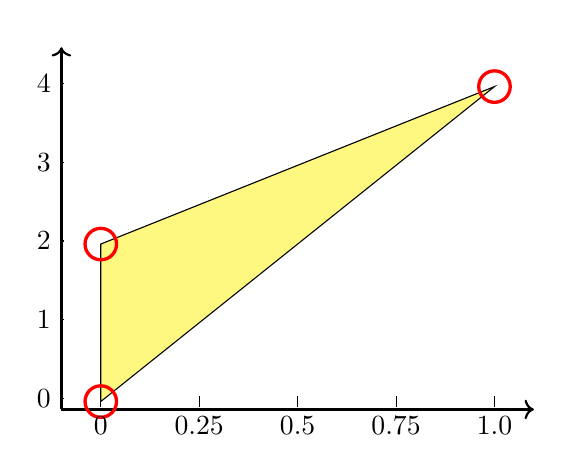
\begin{tikzpicture}
	\begin{scope}[xscale=5, yscale=1]
		% Draw triangle 
		\filldraw[fill=yellow!50] (0,0) -- (0,2) -- (1,4) -- cycle;
		
		% Draw axes
		\draw[thick,->] (-0.1,-0.1) -- (1.1,-0.1) node[right] {};
		\draw[thick,->] (-0.1,-0.1) -- (-0.1,4.5) node[above] {};
	\end{scope}
	
	\foreach \point/\xscale/\yscale in {(0,0)/5/1, (0,2)/5/1, (5,4)/5/1}{
		\draw[red, very thick] \point circle[radius=2mm] node[transform shape, scale=1/\xscale] {};
	}
	% Draw ticks on x-axis and y-axis
	\foreach \x in {0,0.25, 0.5,0.75,1.0} % Adjust or add values for ticks as needed
	\draw[xscale=5] (\x,2pt) -- (\x,-2pt) node[below] {\(\x\)};
	
	\foreach \y in {0,1,...,4} % Adjust or add values for ticks as needed
	\draw (-0.5pt,\y, -0.1) -- (-0.55pt,\y, -0.1) node[left] {\(\y\)};
	
\end{tikzpicture}
\end{center}


\medskip
\noindent
Example 4: Consider the following linear programming problem

\[
	\begin{array}{rl}
		\operatorname{mininize} & -\frac{3}{4} x_{4}+20 x_{5}-\frac{1}{2} x_{6}+6 x_{7} \vspace{2mm}\\
		\text { subject to} & x_{1}+\frac{1}{4} x_{4}-8 x_{5}-x_{6}+9 x_{7}=0 \vspace{2mm}\\
		& x_{2}+\frac{1}{2} x_{4}-12 x_{5}-\frac{1}{2} x_{6}+3 x_{7}=0 \vspace{2mm}\\
		& x_{3}+x_{6}=1 \vspace{2mm}\\
		& x_{1}, \ldots, x_{7} \geq 0 .
	\end{array}
\]

(1) Apply the simplex algorithm to the problem using the rule that \(q\) is the index corresponding to the most negative \(r_{q}\). (As usual, if more than one index \(i\) minimizes \(y_{i 0} / y_{i q}\), let \(p\) be the smallest such index.) Start with \(x_{1}, x_{2}\), and \(x_{3}\) as initial basic variables. Notice that cycling occurs.

(2) Repeat part (1) using Bland's rule for choosing \(q\) and \(p\) :

\begin{equation*}
	\begin{aligned}
		& q=\min \left\{i: r_{i}<0\right\}, \\
		& p=\min \left\{j: y_{j 0} / y_{j q}=\min _{i}\left\{y_{i 0} / y_{i q}: y_{i q}>0\right\}\right\} .
	\end{aligned}
\end{equation*}

\textbf{Short answer}:
(1) We form the tableau for the problem

\begin{equation*}
	\begin{array}{cccccccc}
		1 & 0 & 0 & 1 / 4 & -8 & -1 & 9 & 0 \\
		0 & 1 & 0 & 1 / 2 & -12 & -1 / 2 & 3 & 0 \\
		0 & 0 & 1 & 0 & 0 & 1 & 0 & 1 \\
		0 & 0 & 0 & -3 / 4 & 20 & -1 / 2 & 6 & 0
	\end{array}
\end{equation*}

The above tableau is already in canonical form, and therefore we can process with simplex procedure.

We first pivot about \((1,4)\) th element, to get

\begin{equation*}
	\begin{array}{cccccccc}
		4 & 0 & 0 & 1 & -32 & -4 & 36 & 0 \\
		-2 & 1 & 0 & 0 & 4 & 3 / 2 & -15 & 0 \\
		0 & 0 & 1 & 0 & 0 & 1 & 0 & 1 \\
		3 & 0 & 0 & 0 & -4 & -7 / 2 & 33 & 0
	\end{array}
\end{equation*}

Pivoting about \((2,5)\) th element, we get

\begin{equation*}
	\begin{array}{cccccccc}
		-12 & 8 & 0 & 1 & 0 & 8 & -84 & 0 \\
		-1 / 2 & 1 / 4 & 0 & 0 & 1 & 3 / 8 & -15 / 4 & 0 \\
		0 & 0 & 1 & 0 & 0 & 1 & 0 & 1 \\
		1 & 1 & 0 & 0 & 0 & -2 & 18 & 0
	\end{array}
\end{equation*}

Pivoting about \((1,6)\) th element, we get

\begin{equation*}
	\begin{array}{cccccccc}
		-3 / 2 & 1 & 0 & 1 / 8 & 0 & 1 & -21 / 2 & 0 \\
		1 / 16 & -1 / 8 & 0 & -3 / 64 & 1 & 0 & 3 / 16 & 0 \\
		3 / 2 & -1 & 1 & -1 / 8 & 0 & 0 & 21 / 2 & 1 \\
		-2 & 3 & 0 & 1 / 4 & 0 & 0 & -3 & 0
	\end{array}
\end{equation*}

Pivoting about \((2,7)\) th element, we get

\begin{equation*}
	\begin{array}{cccccccc}
		2 & -6 & 0 & -5 / 2 & 56 & 1 & 0 & 0 \\
		1 / 3 & -2 / 3 & 0 & -1 / 4 & 16 / 3 & 0 & 1 & 0 \\
		-2 & 6 & 1 & 5 / 2 & -56 & 0 & 0 & 1 \\
		-1 & 1 & 0 & -1 / 2 & 16 & 0 & 0 & 0
	\end{array}
\end{equation*}

Pivoting about \((1,1)\) th element, we get

\begin{equation*}
	\begin{array}{cccccccc}
		1 & -3 & 0 & -5 / 4 & 28 & 1 / 2 & 0 & 0 \\
		0 & 1 / 3 & 0 & 1 / 6 & -4 & -1 / 6 & 1 & 0 \\
		0 & 0 & 1 & 0 & 0 & 1 & 0 & 1 \\
		0 & -2 & 0 & -7 / 4 & 44 & 1 / 2 & 0 & 0
	\end{array}
\end{equation*}

Pivoting about \((2,2)\) th element, we get

\begin{equation*}
	\begin{array}{cccccccc}
		1 & 0 & 0 & 1 / 4 & -8 & -1 & 9 & 0 \\
		0 & 1 & 0 & 1 / 2 & -12 & -1 / 2 & 3 & 0 \\
		0 & 0 & 1 & 0 & 0 & 1 & 0 & 1 \\
		0 & 0 & 0 & -3 / 4 & 20 & -1 / 2 & 6 & 0
	\end{array}
\end{equation*}

which is identical to initial tableau. Therefore, cycling occurs.

(2) We start with initial tableau of part (1), and pivot about the \((1,4)\) th element to obtain

\begin{equation*}
	\begin{array}{cccccccc}
		4 & 0 & 0 & 1 & -32 & -4 & 36 & 0 \\
		-2 & 1 & 0 & 0 & 4 & 3 / 2 & -15 & 0 \\
		0 & 0 & 1 & 0 & 0 & 1 & 0 & 1 \\
		3 & 0 & 0 & 0 & -4 & -7 / 2 & 33 & 0
	\end{array}
\end{equation*}

Pivoting about \((2,5)\) th element, we get

\begin{equation*}
	\begin{array}{cccccccc}
		-12 & 8 & 0 & 1 & 0 & 8 & -84 & 0 \\
		-1 / 2 & 1 / 4 & 0 & 0 & 1 & 3 / 8 & -15 / 4 & 0 \\
		0 & 0 & 1 & 0 & 0 & 1 & 0 & 1 \\
		1 & 1 & 0 & 0 & 0 & -2 & 18 & 0
	\end{array}
\end{equation*}

Pivoting about \((1,6)\) th element, we get

\begin{equation*}
	\begin{array}{cccccccc}
		-3 / 2 & 1 & 0 & 1 / 8 & 0 & 1 & -21 / 2 & 0 \\
		1 / 16 & -1 / 8 & 0 & -3 / 64 & 1 & 0 & 3 / 16 & 0 \\
		3 / 2 & -1 & 1 & -1 / 8 & 0 & 0 & 21 / 2 & 1
	\end{array}
\end{equation*}

Pivoting about \((2,1)\) th element, we get

\begin{equation*}
	\begin{array}{cccccccc}
		0 & -2 & 0 & -1 & 24 & 1 & -6 & 0 \\
		1 & -2 & 0 & -3 / 4 & 16 & 0 & 3 & 0 \\
		0 & 2 & 1 & 1 & -24 & 0 & 6 & 1 \\
		0 & -1 & 0 & -5 / 4 & 32 & 0 & 3 & 0
	\end{array}
\end{equation*}

Pivoting about \((3,2)\) th element, we get

\begin{equation*}
	\begin{array}{cccccccc}
		0 & 0 & 1 & 0 & 0 & 1 & 0 & 1 \\
		1 & 0 & 1 & 1 / 4 & -8 & 0 & 9 & 1 \\
		0 & 1 & 1 / 2 & 1 / 2 & -12 & 0 & 3 & 1 / 2 \\
		0 & 0 & 1 / 2 & -3 / 4 & 20 & 0 & 6 & 1 / 2
	\end{array}
\end{equation*}

Pivoting about \((3,2)\) th element, we get

\begin{equation*}
	\begin{array}{cccccccc}
		0 & 0 & 1 & 0 & 0 & 1 & 0 & 1 \\
		1 & -1 / 2 & 3 / 4 & 0 & -2 & 0 & 15 / 2 & 3 / 4 \\
		0 & 2 & 1 & 1 & -24 & 0 & 6 & 1 \\
		0 & 3 / 2 & 5 / 4 & 0 & 2 & 0 & 21 / 2 & 5 / 4
	\end{array}
\end{equation*}

The reduced cost coefficient are all nonnegative. Hence, the optimal solution to the problem is \(\left[\begin{array}{lllllll}3 / 4 & 0 & 0 & 1 & 0 & 1 & 0\end{array}\right]^{\top}\). The corresponding optimal cost is \(-5 / 4\).

%------------------------------------------------------%
%------------------------------------------------------%
\section{Linear Programming and its Duality}
%------------------------------------------------------%
%------------------------------------------------------%

%------------------------------------------------------%
\subsection{Practice problems}

Example 1
\[
	\begin{array}{rl}
		\operatorname{maximize} & 5 x_{1}+2 x_{2} \vspace{2mm}\\
		\text { subject to} & x_{1}+x_{2}+x_{3}=5 \vspace{2mm}\\
		& -3 x_{1}+2 x_{2}-x_{4}=-5 \vspace{2mm}\\
		& x_{i} \geq 0, \quad i=1,2,3,4 .
	\end{array}
\]

\textbf{Short answer}:
We transform the problem into the following equivalent problem,

\[
	\begin{array}{rl}
		\operatorname{minimize} & -5 x_{1}-2 x_{2} \vspace{2mm}\\
		\text { subject to} & x_{1}+x_{2}+x_{3}=5 \vspace{2mm}\\
		& 3 x_{1}-2 x_{2}+x_{4}=5 \vspace{2mm}\\
		& x_{i} \geq 0, i=1,2,3,4 .
	\end{array}
\]

We form the tableau for the problem and process with simplex procedure.

\begin{equation*}
	\begin{array}{cccc|c}
		1 & 1 & 1 & 0 & 5 \\
		3 & -2 & 0 & 1 & 5 \\
		\hline-5 & -2 & 0 & 0 & 0
	\end{array}
\end{equation*}

We first pivot about \((2,1)\) th element, to get

\begin{equation*}
	\begin{array}{cccc|c}
		0 & 5 / 3 & 1 & -1 / 3 & 10 / 3 \\
		1 & -2 / 3 & 0 & 1 / 3 & 5 / 3 \\
		\hline 0 & -16 / 3 & 0 & 5 / 3 & 25 / 3
	\end{array}
\end{equation*}

\begin{center}
	\begin{tabular}{cccc|c}
		0 & 1 & \(3 / 5\) & \(-1 / 5\) & 2 \\
		1 & 0 & \(2 / 5\) & \(1 / 5\) & 3 \\
		\hline
		0 & 0 & \(16 / 5\) & \(3 / 5\) & 19 \\
		\hline
	\end{tabular}
\end{center}

We then pivot about \((1,2)\) th element, to get the tableau above.

We have the optimized basic feasible solution as \(\boldsymbol{x}=\left[\begin{array}{llll}3 & 2 & 0 & 0\end{array}\right]^{\top}\). The optimal value of \(5 x_{1}+2 x_{2}\) is 19 .


\medskip
\noindent
Example 2. Find the dual problem corresponding to the following primal problem:

\[
	\begin{array}{rl}
		\operatorname{minimize} & c^{\top} x \vspace{2mm}\\
		\text { subject to} & A_{1} x \geq b_{1} \vspace{2mm}\\
		& A_{2} x \leq b_{2} \vspace{2mm}\\
		& A_{3} x=b_{3} \vspace{2mm}\\
		& \boldsymbol{x} \geq 0 .
	\end{array}
\]

\textbf{Short answer}:

We transform the given problem into its standard form:

\[
	\begin{array}{rl}
		\operatorname{ minimize} & c^{\top} x \vspace{2mm} \\
		\text { subject to} & A_{1} x \geq b_{1} \vspace{2mm} \\
		& -A_{2} x \geq-b_{2} \vspace{2mm} \\
		& A_{3} x \geq b_{3} \vspace{2mm} \\
		& -A_{3} x \geq-b_{3} \vspace{2mm} \\
		& \boldsymbol{x} \geq 0 .
	\end{array}
\]

The dual problem is then:

\begin{equation*}
	\begin{aligned}
		& \text { maximize }\left[\begin{array}{llll}
			u^{\top} & v^{\top} & w^{\top} & \lambda^{\top}
		\end{array}\right]\left[\begin{array}{c}
			b_{1} \\
			-b_{2} \\
			b_{3} \\
			-b_{3}
		\end{array}\right] \\
		& \text { subject to }\left[\begin{array}{llll}
			u^{\top} & v^{\top} & w^{\top} & \lambda^{\top}
		\end{array}\right]\left[\begin{array}{c}
			A_{1} \\
			-A_{2} \\
			A_{3} \\
			-A_{3}
		\end{array}\right] \leq c^{\top}
	\end{aligned}
\end{equation*}

\begin{equation*}
	u, v, w, \lambda \geq 0 .
\end{equation*}


\medskip
\noindent
Example 3. Convert the following optimization problem into a linear programming problem and solve it;

\[
	\begin{array}{rl}
		\text { maximize} & -\left|x_{1}\right|-\left|x_{2}\right|-\left|x_{3}\right| \vspace{2mm}\\
		\text { subject to } & {\left[\begin{array}{ccc}
				1 & 1 & -1 \\
				0 & -1 & 0
			\end{array}\right]\left[\begin{array}{l}
				x_{1} \\
				x_{2} \\
				x_{3}
			\end{array}\right]=\left[\begin{array}{l}
				2 \\
				1
			\end{array}\right] .}
	\end{array}
\]

Construct its dual program and solve it.

\textbf{Short answer}:

We introduce two sets of non-negative variables: \(x_{i}^{+} \geq 0, x_{i}^{-} \geq 0\), \(i=1,2,3\). We can then represent the optimization problem in the form

\[
	\begin{array}{cl}
		\text { minimize} &
		\left(x_{1}^{+}+x_{1}^{-}\right)+\left(x_{2}^{+}+x_{2}^{-}\right)+\left(x_{3}^{+}+x_{3}^{-}\right) \vspace{2mm} \\
		\text {subject to} & {\left[\begin{array}{cccccc}
				1 & 1 & -1 & -1 & -1 & 1 \\
				0 & -1 & 0 & 0 & 1 & 0
			\end{array}\right]\left[\begin{array}{l}
				x_{1}^{+} \\
				x_{2}^{+} \\
				x_{3}^{+} \\
				x_{1}^{-} \\
				x_{2}^{-} \\
				x_{3}^{-}
			\end{array}\right]=\left[\begin{array}{l}
				2 \\
				1
			\end{array}\right]} \\
		& x_{i}^{+}, x_{i}^{-} \geq 0 .
	\end{array}
\]

We form the initial tableau,

\[
	\begin{array}{cccccc|c}
		1 & 1 & -1 & -1 & -1 & 1 & 2 \\
		0 & -1 & 0 & 0 & 1 & 0 & 1 \\
		\hline 1 & 1 & 1 & 1 & 1 & 1 & 0
	\end{array}
\]

There is no apparent basic feasible solution. We add the second row to the first one to obtain,

\[
	\begin{array}{cccccc|c}
		1 & 0 & -1 & -1 & 0 & 1 & 3 \\
		0 & -1 & 0 & 0 & 1 & 0 & 1 \\
		\hline 1 & 1 & 1 & 1 & 1 & 1 & 0
	\end{array}
\]

We next calculate the reduced cost coefficients,

\[
	\begin{array}{cccccc|c}
		1 & 0 & -1 & -1 & 0 & 1 & 3 \\
		0 & -1 & 0 & 0 & 1 & 0 & 1 \\
		\hline 0 & 2 & 2 & 2 & 0 & 0 & -4
	\end{array}
\]

We have zeros under the basic columns. The reduced cost coefficients are all non-negative. The optimal solution is,

\[
	\boldsymbol{x}^{*}=\left[\begin{array}{llllll}
		3 & 0 & 0 & 0 & 1 & 0
	\end{array}\right]^{\top} .
\]

The optimal solution to the original problem is \(\boldsymbol{x}^{*}=\left[\begin{array}{lll}3 & -1 & 0\end{array}\right]^{\top}\).

The dual of the above linear program is

\[
	\begin{array}{cl}
	\operatorname{maximize} &  2 \lambda_{1}+\lambda_{2} \\
	\text{ subject to} &  
		\left[\begin{array}{ll}\lambda_{1} & \lambda_{2}\end{array}\right]
		\left[\begin{array}{cccccc}1 & 1 & -1 & -1 & -1 & 1 \\ 0 & -1 & 0 & 0 & 1 & 0\end{array}\right] \leq
		\left[\begin{array}{llllll}1 & 1 & 1 & 1 & 1 & 1\end{array}\right].
	\end{array}
\]

The optimal solution to the dual is,

\[
	\begin{aligned}
		\boldsymbol{\lambda}^{* \top} & =\boldsymbol{c}_{\boldsymbol{B}}^{\top} \boldsymbol{B}^{-1} \\
		& =\left[\begin{array}{ll}
			1 & 1
		\end{array}\right]\left[\begin{array}{cc}
			1 & -1 \\
			0 & 1
		\end{array}\right]^{-1} \\
		& =\left[\begin{array}{ll}
			1 & 2
		\end{array}\right] .
	\end{aligned}
\]


% Part 4: Nonlinear Constrained Optimization
%------------------------------------------------------%
%------------------------------------------------------%
\section{FONC, SONC, SOSC for unconstrained optimization problem}
%------------------------------------------------------%
%------------------------------------------------------%

%------------------------------------------------------%
\subsection{Practice problems}
\begin{enumerate}
	\item Find minimizers and maximizers of the function,	
	\[
		f\left(x_{1}, x_{2}\right)=\frac{1}{3} x_{1}^{3}-4 x_{1}+\frac{1}{3} x_{2}^{3}-9 x_{2} .
	\]

\end{enumerate}


\textbf{Short answer}:

Because there are no constraints on \(x_{1}\) or \(x_{2}\), we can utilize conditions for unconstrained optimization. To proceed, we first compute the function gradient and find the critical points, that is, the points that satisfy the FONC,

\[
	\nabla f\left(x_{1}, x_{2}\right)=0 .
\]

The components of the gradient \(\nabla f\left(x_{1}, x_{2}\right)\) are

\[
	\frac{\partial f}{\partial x_{1}}=x_{1}^{2}-4 \text { and } \frac{\partial f}{\partial x_{2}}=x_{2}^{2}-9 .
\]

Thus there are four critical points,

\[
	\boldsymbol{x}^{(1)}=\left[\begin{array}{l}
		2 \\
		3
	\end{array}\right], \boldsymbol{x}^{(2)}=\left[\begin{array}{c}
		2 \\
		-3
	\end{array}\right], \boldsymbol{x}^{(3)}=\left[\begin{array}{c}
		-2 \\
		3
	\end{array}\right], \text { and } \boldsymbol{x}^{(4)}=\left[\begin{array}{c}
		-2 \\
		-3
	\end{array}\right] .
\]

We next compute the Hessian matrix of the function \(f\),

\[
	\boldsymbol{F}(\boldsymbol{x})=\left[\begin{array}{cc}
		2 x_{1} & 0 \\
		0 & 2 x_{2}
	\end{array}\right]
\]

Note that \(\boldsymbol{F}\left(\boldsymbol{x}^{(1)}\right) \succ 0\) and therefore, \(\boldsymbol{x}^{(1)}\) is a strict local minimizer. Next, \(\boldsymbol{F}\left(\boldsymbol{x}^{(4)}\right) \prec 0\) and therefore, \(\boldsymbol{x}^{(4)}\) is a strict local maximizer. The Hessian is indefinite at \(\boldsymbol{x}^{(2)}\) and \(\boldsymbol{x}^{(3)}\) and so these points are neither maximizers nor minimizers.

\begin{enumerate}
	\setcounter{enumi}{1}
	\item In some of the optimization methods, when minimizing a given function \(f(\boldsymbol{x})\), we select an initial guess \(\boldsymbol{x}^{(0)}\) and a real symmetric positive definite matrix \(\boldsymbol{H}_{0}\). Then we compute \(\boldsymbol{d}^{(k)}=-\boldsymbol{H}_{k} g^{(k)}\), where \(\boldsymbol{g}^{(k)}=\nabla f\left(\boldsymbol{x}^{(k)}\right)\), and \(\boldsymbol{x}^{(k+1)}=\boldsymbol{x}^{(k)}+\alpha_{k} \boldsymbol{d}^{(k)}\), where
	\[
		\alpha_{k}=\arg \min _{\alpha \geq 0} f\left(\boldsymbol{x}^{(k)}+\alpha \boldsymbol{d}^{(k)}\right) .
	\]

	Suppose that the function we wish to minimize is a standard quadratic of the form,
	
	\[
		f(\boldsymbol{x})=\frac{1}{2} \boldsymbol{x}^{\top} \boldsymbol{Q} \boldsymbol{x} - \boldsymbol{x}^{\top} \boldsymbol{b}+c, \quad \boldsymbol{Q}=\boldsymbol{Q}^{\top} \succ 0 .
	\]
	
	(1) Find a closed form expression for \(\alpha_{k}\) in terms of \(\boldsymbol{Q}, \boldsymbol{H}_{k}, \boldsymbol{g}^{(k)}\), and \(\boldsymbol{d}^{(k)}\).
	
	(2) Give a sufficient condition on \(\boldsymbol{H}_{k}\) for \(\alpha_{k}\) to be positive.

\end{enumerate}


\textbf{Short answer}:

(1) We have

\[
	f\left(\boldsymbol{x}^{(k)}+\alpha \boldsymbol{d}^{(k)}\right) = 
	\frac{1}{2}\left(\boldsymbol{x}^{(k)}+\alpha \boldsymbol{d}^{(k)}\right)^{\top} \boldsymbol{Q} \left(\boldsymbol{x}^{(k)}+\alpha \boldsymbol{d}^{(k)}\right)-\left(\boldsymbol{x}^{(k)}+\alpha \boldsymbol{d}^{(k)}\right)^{\top} \boldsymbol{b}+c .
\]

Using the chain rule, we obtain

\[
	\frac{d}{d \alpha} f\left(\boldsymbol{x}^{(k)}+\alpha \boldsymbol{d}^{(k)}\right) = \left(\boldsymbol{x}^{(k)}+\alpha \boldsymbol{d}^{(k)}\right)^{\top} \boldsymbol{Q} \boldsymbol{d}^{(k)}-\boldsymbol{d}^{(k)^{\top}} \boldsymbol{b} .
\]

Equating the above to zero and solving for \(\alpha\) gives

\[
	\left(\boldsymbol{x}^{(k)^{\top}} \boldsymbol{Q}-\boldsymbol{b}^{\top}\right) \boldsymbol{d}^{(k)}=-\alpha \boldsymbol{d}^{(k)^{\top}} \boldsymbol{Q} \boldsymbol{d}^{(k)} .
\]

Taking into account that \(\boldsymbol{g}^{(k)^{\top}} = \boldsymbol{x}^{(k)^{\top}} \boldsymbol{Q}-\boldsymbol{b}^{\top}\) and that \(\boldsymbol{d}^{(k)^{\top}} \boldsymbol{Q} \boldsymbol{d}^{(k)}>0\) for \(\boldsymbol{g}^{(k)} \neq 0\), we obtain

\[
	\alpha_{k} = -\frac{\boldsymbol{g}^{(k)^{\top}} \boldsymbol{d}^{(k)}}{\boldsymbol{d}^{(k)^{\top}} \boldsymbol{Q} \boldsymbol{d}^{(k)}} = \frac{\boldsymbol{g}^{(k)^{\top}} \boldsymbol{H}_{k} \boldsymbol{g}^{(k)}}{\boldsymbol{d}^{(k)^{\top}} \boldsymbol{Q} \boldsymbol{d}^{(k)}} .
\]

(2) The matrix \(\boldsymbol{Q}\) is symmetric and positive definite; hence \(\alpha_{k}>0\) if \(\boldsymbol{H}_{k}=\) \(\boldsymbol{H}_{k}^{\top} \succ 0\).

%------------------------------------------------------%
%------------------------------------------------------%
\section{Lagrange's condition and its application}
%------------------------------------------------------%
%------------------------------------------------------%

%------------------------------------------------------%
\subsection{Practice problems}
\begin{enumerate}
	\item Find all maximizers of the function
	\[
	f\left(x_{1}, x_{2}\right)=\frac{18 x_{1}^{2}-8 x_{1} x_{2}+12 x_{2}^{2}}{2 x_{1}^{2}+2 x_{2}^{2}} .
	\]
\end{enumerate}


\textbf{Short answer}:

We observe that \(f\left(x_{1}, x_{2}\right)\) is a ratio of two quadratic functions, that is, we can represent \(f\left(x_{1}, x_{2}\right)\) as

\[
	f\left(x_{1}, x_{2}\right)=\frac{\boldsymbol{x}^{\top} \boldsymbol{Q} \boldsymbol{x}}{\boldsymbol{x}^{\top} \boldsymbol{P} \boldsymbol{x}} .
\]

Therefore, if a point \(\boldsymbol{x}\) is a maximizer of \(f\left(x_{1}, x_{2}\right)\) then so is any nonzero multiple of this point because

\begin{equation*}
	\frac{(t \boldsymbol{x})^{\top} \boldsymbol{Q}(t \boldsymbol{x})}{(t \boldsymbol{x})^{\top} \boldsymbol{P}(t \boldsymbol{x})}=\frac{t^{2} \boldsymbol{x}^{\top} \boldsymbol{Q} \boldsymbol{x}}{t^{2} \boldsymbol{x}^{\top} \boldsymbol{P} \boldsymbol{x}}=\frac{\boldsymbol{x}^{\top} \boldsymbol{Q} \boldsymbol{x}}{\boldsymbol{x}^{\top} \boldsymbol{P} \boldsymbol{x}} .
\end{equation*}

Thus any nonzero multiple of a solution is also a solution. To proceed, represent the original problem in an equivalent form,

\[
	\begin{array}{rl}
		\operatorname{maximize} & \boldsymbol{x}^{\top} \boldsymbol{Q} \boldsymbol{x}=18 x_{1}^{2}-8 x_{1} x_{2}+12 x_{2}^{2} \vspace{2mm}\\
		\text { subject to} & \boldsymbol{x}^{\top} \boldsymbol{P} \boldsymbol{x}=2 x_{1}^{2}+2 x_{2}^{2}=1 .
	\end{array}
\]

We apply the Lagrange's method to solve the problem. We form the Lagrangian function,

\[
	l(\boldsymbol{x}, \boldsymbol{\lambda})=f(\boldsymbol{x})+ \lambda h(\boldsymbol{x}),
\]

compute its gradient and find critical points. We have,

\[
	\begin{aligned}
		\nabla_{\boldsymbol{x}} l (\boldsymbol{x}, \boldsymbol{\lambda}) & =\nabla_{\boldsymbol{x}}\left(\boldsymbol{x}^{\top}\left[\begin{array}{cc}
			18 & -4 \\
			-4 & 12
		\end{array}\right] \boldsymbol{x}+\lambda\left(1-\boldsymbol{x}^{\top}\left[\begin{array}{ll}
			2 & 0 \\
			0 & 2
		\end{array}\right] \boldsymbol{x}\right)\right) \\
		& =2\left[\begin{array}{cc}
			18 & -4 \\
			-4 & 12
		\end{array}\right] \boldsymbol{x}-2 \lambda \left[\begin{array}{cc}
			2 & 0 \\
			0 & 2
		\end{array}\right] \boldsymbol{x} \\
		& =\boldsymbol{0} .
	\end{aligned}
\]

We represent the above in an equivalent form,

\[
	\left(\lambda \boldsymbol{I}_{2}-\left[\begin{array}{ll}
		2 & 0 \\
		0 & 2
	\end{array}\right]^{-1}\left[\begin{array}{cc}
		18 & -4 \\
		-4 & 12
	\end{array}\right]\right) \boldsymbol{x}= \boldsymbol{0}.
\]

That is, solving the problem is being reduced to solving an eigenvalue-eigenvector problem,

\[
	\left(\lambda \boldsymbol{I}_{2}-\left[\begin{array}{cc}
		9 & -2 \\
		-2 & 6
	\end{array}\right]\right) \boldsymbol{x}=\left[\begin{array}{cc}
		\lambda-9 & 2 \\
		2 & \lambda-6
	\end{array}\right] \boldsymbol{x}=\boldsymbol{0} .
\]

The characteristic polynomial is

\[
	\lambda^{2}-15 \lambda+50=(\lambda-5)(\lambda-10) .
\]

The eigenvalues are 5 and 10 . Because we are interested in finding a maximizer, we conclude that the value of the maximized function is 10 , while the corresponding maximizer corresponds to an appropriate scaled, to satisfy the constraint, eigenvector of this eigenvalue. An eigenvector can easily be found by taking any nonzero column of the adjoint matrix of

\[
	10 \boldsymbol{I}_{2}-\left[\begin{array}{cc}
		9 & -2 \\
		-2 & 6
	\end{array}\right] = \left[\begin{array}{cc}
	1  & 2 \\
	2 & 4
	\end{array}\right].
\]

Thus

\[
	\sqrt{0.1}\left[\begin{array}{c}
		-2 \\
		1
	\end{array}\right]
\]

is a maximizer for the equivalent problem. Any multiple of the above vector is a solution of the original maximization problem.

\begin{enumerate}
	\setcounter{enumi}{1}
	\item Consider the following model of a discrete-time system,
	\[
		x(k+1)=x(k)+2 u(k),
	\]
\end{enumerate}

where \(x(0)=3\), and \(0 \leq k \leq 2\). Use the Lagrange multiplier approach to calculate the optimal control sequence

\[
	\{u(0), u(1), u(2)\}
\]

that transfers the initial state \(x(0)\) to \(x(3)=9\) while minimizing the performance index

\[
	J=\frac{1}{2} \sum_{k=0}^{2} u(k)^{2}=\frac{1}{2} \boldsymbol{u}^{\top} \boldsymbol{u} .
\]

\textbf{Short answer}: 

The composite input vector,

\[
	\boldsymbol{u}=\left[\begin{array}{lll}
		u(0) & u(1) & u(2)
	\end{array}\right]^{\top} .
\]

The performance index \(J\) is \(J=\dfrac{1}{2} \boldsymbol{u}^{\top} \boldsymbol{u}\). To obtain the constraint \(\boldsymbol{A} \boldsymbol{u}=\boldsymbol{b}\), where \(\boldsymbol{A} \in \mathbb{R}^{1 \times 3}\), we proceed as follows. First, we write

\[
	\begin{aligned}
		x(2) & =x(1)+2 u(1) \\
		& =x(0)+2 u(0)+2 u(1) .
	\end{aligned}
\]

Using the above, we obtain

\[
	\begin{aligned}
		x(3) & =x(2)+2 u(2) \\
		& =x(0)+2 u(0)+2 u(1)+2 u(2) \\
		& =9 .
	\end{aligned}
\]

We represent the above in the format \(\boldsymbol{A} \boldsymbol{u}=\boldsymbol{b}\) as follows

\[
	\left[\begin{array}{lll}
		2 & 2 & 2
	\end{array}\right]\left[\begin{array}{l}
		u(0) \\
		u(1) \\
		u(2)
	\end{array}\right]=6 .
\]

Thus we formulate the problem of finding the optimal control sequence as a constrained optimization problem

\[
	\begin{array}{rl}
		\operatorname{minimize} & \dfrac{1}{2} \boldsymbol{u}^{\top} \boldsymbol{u} \vspace{2mm}\\
		\text { subject to} & \boldsymbol{A} \boldsymbol{u}=\boldsymbol{b} .
	\end{array}
\]

To solve the above problem, we form the Lagrangian

\[
	l(\boldsymbol{u}, \boldsymbol{\lambda} )=\frac{1}{2} \boldsymbol{u}^{\top} \boldsymbol{u}+ \boldsymbol{\lambda}^{\top} (\boldsymbol{A} \boldsymbol{u}-\boldsymbol{b}),
\]

where \(\lambda\) is the Lagrange multiplier. Applying the Lagrange's first-order condition yields

\[
	\boldsymbol{u}+\boldsymbol{A}^{\top} \boldsymbol{\lambda}=\boldsymbol{0} \text { and } \boldsymbol{A} \boldsymbol{u}=\boldsymbol{b} .
\]

From the first of the above conditions, we calculate, \(\boldsymbol{u}=-\boldsymbol{A}^{\top} \boldsymbol{\lambda} \). Substituting the above into the second of the Lagrange conditions gives

\[
	\boldsymbol{\lambda}=-\left(\boldsymbol{A} \boldsymbol{A}^{\top}\right)^{-1} \boldsymbol{b} .
\]

Combining the last two equations, we obtain a closed-form formula for the optimal input sequence

\[
	\boldsymbol{u}=\boldsymbol{A}^{\top}\left(\boldsymbol{A} \boldsymbol{A}^{\top}\right)^{-1} \boldsymbol{b} .
\]

In this problem,

\[
	u=\left[\begin{array}{l}
		u(0) \\
		u(1) \\
		u(2)
	\end{array}\right]=\frac{\boldsymbol{b}}{\left(\boldsymbol{A} \boldsymbol{A}^{\top}\right)} \boldsymbol{A}^{\top}=\left[\begin{array}{l}
		1 \\
		1 \\
		1
	\end{array}\right] .
\]

\begin{enumerate}
	\setcounter{enumi}{2}
	\item Find minimizers and maximizers of the function,
	\[
		f(\boldsymbol{x})=\left(\boldsymbol{a}^{\top} \boldsymbol{x}\right)\left(\boldsymbol{b}^{\top} \boldsymbol{x}\right), \boldsymbol{x} \in \mathbb{R}^{3},
	\]

	subject to
	\[
		\begin{aligned}
			& x_{1}+x_{2}=0 \\
			& x_{2}+x_{3}=0
		\end{aligned}
	\]

	where
	
	\[
		\boldsymbol{a}=\left[\begin{array}{l}
			0 \\
			1 \\
			0
		\end{array}\right] \text { and } \boldsymbol{b}=\left[\begin{array}{l}
			1 \\
			0 \\
			1
		\end{array}\right] .
	\]
\end{enumerate}

\textbf{Short answer}: 

We form the Lagrangian

\[
	l(\boldsymbol{x}, \boldsymbol{\lambda} )=\frac{1}{2} \boldsymbol{x}^{\top}\left(\boldsymbol{a} \boldsymbol{b}^{\top}+\boldsymbol{b} \boldsymbol{a}^{\top}\right) \boldsymbol{x}+\lambda_{1}\left(x_{1}+x_{2}\right)+\lambda_{2}\left(x_{2}+x_{3}\right) .
\]

The Lagrange conditions take the form,

\[
	\begin{aligned}
		\nabla_{\boldsymbol{x}} l (\boldsymbol{x}, \boldsymbol{\lambda})
		& =\left(\boldsymbol{a} \boldsymbol{b}^{\top}+\boldsymbol{b} \boldsymbol{a}^{\top}\right) \boldsymbol{x}+\left[\begin{array}{ll}
			\nabla_{\boldsymbol{x}} h_{1}(\boldsymbol{x}) & \nabla_{\boldsymbol{x}} h_{2}(\boldsymbol{x})
		\end{array}\right] \boldsymbol{\lambda} \\
		& =\left[\begin{array}{lll}
			0 & 1 & 0 \\
			1 & 0 & 1 \\
			0 & 1 & 0
		\end{array}\right] \boldsymbol{x}+\left[\begin{array}{ll}
			1 & 0 \\
			1 & 1 \\
			0 & 1
		\end{array}\right] \boldsymbol{\lambda} \\
		& =\left[\begin{array}{l}
			0 \\
			0 \\
			0
		\end{array}\right], \\
		h(\boldsymbol{x})
		& =\left[\begin{array}{l}
			x_{1}+x_{2} \\
			x_{2}+x_{3}
		\end{array}\right]=\left[\begin{array}{l}
			0 \\
			0
		\end{array}\right] .
	\end{aligned}
\]

It is easy to see that \(\boldsymbol{x}^{*}=\left[\begin{array}{ll}0 & 0\end{array}\right]^{\top}\) and \(\boldsymbol{\lambda}^{*}=\left[\begin{array}{ll}0 & 0\end{array}\right]^{\top}\) satisfy the Lagrange, FONC conditions. The Hessian of the lagrangian is

\[
	\boldsymbol{L}\left(\boldsymbol{x}^{*}, \boldsymbol{\lambda}^{*}\right)=\boldsymbol{a} \boldsymbol{b}^{\top}+\boldsymbol{b} \boldsymbol{a}^{\top}=\left[\begin{array}{ccc}
		0 & 1 & 0 \\
		1 & 0 & 1 \\
		0 & 1 & 0
	\end{array}\right]
\]

and the tangent space

\[
	T\left(\boldsymbol{x}^{*}\right)=\left\{\boldsymbol{y}: \boldsymbol{y} = c \left[\begin{array}{c}
		1 \\
		-1 \\
		1
	\end{array}\right], c \in \mathbb{R}\right\} .
\]

To verify if the critical point satisfies the SOSC, we evaluate

\[
	\boldsymbol{y}^{\top} \boldsymbol{L} \left(\boldsymbol{x}^{*}, \boldsymbol{\lambda}^{*}\right) \boldsymbol{y}=-4 c^{2}<0 .
\]

Thus the critical point is a strict local maximizer.

%------------------------------------------------------%
%------------------------------------------------------%
\section{KKT condition and its application}
%------------------------------------------------------%
%------------------------------------------------------%

%------------------------------------------------------%
\subsection{Practice problems}
\begin{enumerate}
	\item Consider the optimization problem
	\[
		\begin{array}{rl}
			\operatorname{minimize} & x_{1}^{2}+4 x_{2}^{2} \vspace{2mm} \\
			\text { subject to} & x_{1}^{2}+2 x_{2}^{2} \geq 4 .
		\end{array}
	\]
	
	(1) Find all points that satisfy the KKT conditions.
	
	(2) Apply the SOSC to determine the nature of the critical points from the previous part.

\end{enumerate}

\textbf{Short answer}:

We form the Lagrangian function,

\[
	l(\boldsymbol{x}, \mu)=x_{1}^{2}+4 x_{2}^{2}+\mu\left(4-x_{1}^{2}-2 x_{2}^{2}\right) .
\]

The KKT conditions take the form,

\[
	\begin{aligned}
		& D_{\boldsymbol{x}} l(\boldsymbol{x}, \mu)=\left[\begin{array}{ll}
			2 x_{1}-2 \mu x_{1} & 8 x_{2}-4 \mu x_{2}
		\end{array}\right]=\boldsymbol{0}^{\top} \\
		& \mu\left(4-x_{1}^{2}-2 x_{2}^{2}\right)=0 \\
		& \mu>0 \\
		& 4-x_{1}^{2}-2 x_{2}^{2} \leq 0 .
	\end{aligned}
\]

From the first of the above equality, we obtain \((1-\mu) x_{1}=0\) and \((2-\mu) x_{2}=0\). We first consider the case when \(\mu=0\). Then, we obtain the point \(\boldsymbol{x}^{(1)}=0\), which does not satisfy the constraints.

The next case is when \(\mu=1\). Then we have \(x_{2}=0\) and using \(\mu\left(4-x_{1}^{2}-\right.\) \(\left.2 x_{2}^{2}\right)=0\) gives

\[
	\boldsymbol{x}^{(2)}=\left[\begin{array}{l}
		2 \\
		0
	\end{array}\right] \text { and } \boldsymbol{x}^{(3)}=\left[\begin{array}{c}
		-2 \\
		0
	\end{array}\right] .
\]

For the case when \(\mu=2\), we have to have \(x_{1}=0\) and we get

\[
	\boldsymbol{x}^{(4)}=\left[\begin{array}{c}
		0 \\
		\sqrt{2}
	\end{array}\right] \text { and } \boldsymbol{x}^{(5)}=\left[\begin{array}{c}
		0 \\
		-\sqrt{2}
	\end{array}\right] .
\]

The Hessian of \(l\) is

\[
	\boldsymbol{L}=\left[\begin{array}{ll}
		2 & 0 \\
		0 & 8
	\end{array}\right]+\mu\left[\begin{array}{cc}
		-2 & 0 \\
		0 & -4
	\end{array}\right]
\]

When \(\mu=1\),

\[
	\boldsymbol{L}=\left[\begin{array}{ll}
		0 & 0 \\
		0 & 4
	\end{array}\right]
\]

We next find the subspace

\[
	\begin{aligned}
		\tilde{T} & =T=\left\{\boldsymbol{y}: \left[\begin{array}{ll} 
			\pm 4 & 0
		\end{array}\right] \boldsymbol{y}=0\right\} \\
		& =\left\{\boldsymbol{y}=a\left[\begin{array}{ll}
			0 & 1
		\end{array}\right]^{\top}: a \in \mathbb{R}\right\} .
	\end{aligned}
\]

We then check for positive definiteness of \(\boldsymbol{L}\) on \(\tilde{T}\),

\[
	\boldsymbol{y}^{\top} \boldsymbol{L} \boldsymbol{y}=a^{2}\left[\begin{array}{ll}
		0 & 1
	\end{array}\right]\left[\begin{array}{ll}
		0 & 0 \\
		0 & 4
	\end{array}\right]\left[\begin{array}{l}
		0 \\
		1
	\end{array}\right]=4 a^{2}>0 .
\]

Hence, \(\boldsymbol{x}^{(2)}\) and \(\boldsymbol{x}^{(3)}\) satisfy the SOSC to be strict local minimizers. When \(\mu=2\),

\[
	\boldsymbol{L}=\left[\begin{array}{cc}
		-2 & 0 \\
		0 & 0
	\end{array}\right]
\]
and

\[
	T=\left\{\boldsymbol{y}=a\left[\begin{array}{ll}
		1 & 0
	\end{array}\right]^{\top}: a \in \mathbb{R}\right\}
\]

We have

\[
	\boldsymbol{y}^{\top} \boldsymbol{L} \boldsymbol{y}=-2 a^{2}<0 .
\]

Thus, \(\boldsymbol{x}^{(4)}\) and \(\boldsymbol{x}^{(5)}\) do not satisfy the SONC to be minimizers. In summary, only \(\boldsymbol{x}^{(2)}\) and \(\boldsymbol{x}^{(3)}\) are strict local minimizers.

\begin{enumerate}
	\setcounter{enumi}{1}
	\item Consider the following constraints on \(\mathbb{R}^{2}\) :

	\[
		\begin{aligned}
			& h\left(x_{1}, x_{2}\right)=\left(x_{1}-2\right)^{2}=0 \\
			& g\left(x_{1}, x_{2}\right)=\left(x_{2}+1\right)^{3} \leq 0 .
		\end{aligned}
	\]
	
	(1) Find the set of feasible points.
	
	(2) Are the feasible points regular or not. Justify your answer.

\end{enumerate}

\textbf{Short answer}:

The feasible set consists of the points

\[
	\boldsymbol{x}=\left[\begin{array}{l}
		2 \\
		a
	\end{array}\right], a \leq-1 .
\]

We next find the gradients,

\[
	\nabla h(\boldsymbol{x})=\left[\begin{array}{c}
		2\left(x_{1}-2\right) \\
		0
	\end{array}\right] \text { and } \nabla g(\boldsymbol{x})=\left[\begin{array}{c}
		0 \\
		3\left(x_{2}+1\right)^{2}
	\end{array}\right]
\]

All feasible points are not regular because at the above points the gradient of \(h\) and \(g\) are not linearly independent. There are no regular points of the constraints.

\begin{enumerate}
	\setcounter{enumi}{2}
	\item Show that the two problems below are dual by showing the equivalence of the KKT conditions:
	\begin{mini*}|l|
		{\boldsymbol{x}}{\boldsymbol{c}^{\top} \boldsymbol{x}}
		{}{}
		\addConstraint{\boldsymbol{A} \boldsymbol{x} \geq \boldsymbol{b}}
		\addConstraint{\boldsymbol{x} \geq 0.}{}
	\end{mini*}

	and
	\begin{maxi*}|l|
		{\boldsymbol{\lambda}}{\boldsymbol{b}^{\top} \boldsymbol{\lambda}}
		{}{}
		\addConstraint{\boldsymbol{A}^{\top} \boldsymbol{\lambda} \geq \boldsymbol{c}}
		\addConstraint{\boldsymbol{\lambda} \geq 0.}{}
	\end{maxi*}

\end{enumerate}

\textbf{Short answer}:

It is sufficient to show that the two linear programs have identical KKT conditions. For the first linear program, let \(\boldsymbol{\mu}\) be the vector of Lagrangian multipliers associated with \(\boldsymbol{A} \boldsymbol{x}-\boldsymbol{b} \geq \boldsymbol{0}\), and \(\boldsymbol{s}\) be the vector of multipliers associated with \(\boldsymbol{x} \geq 0\). The Lagrangian function is then

\begin{equation*}
	L_{1}(\boldsymbol{x}, \boldsymbol{\mu}, \boldsymbol{s})=\boldsymbol{c}^{\top} \boldsymbol{x}-\boldsymbol{\mu}^{\top}(\boldsymbol{A} \boldsymbol{x}-\boldsymbol{b})-\boldsymbol{s}^{\top} \boldsymbol{x} .
\end{equation*}

The KKT conditions are

\[
	\begin{aligned}
		\boldsymbol{A}^{\top} \boldsymbol{\mu}+\boldsymbol{s} & = \boldsymbol{c} \\
		\boldsymbol{A} \boldsymbol{x} & \geq \boldsymbol{b} \\
		\boldsymbol{x} & \geq \boldsymbol{0} \\
		\boldsymbol{\mu} & \geq \boldsymbol{0} \\
		\boldsymbol{s} & \geq \boldsymbol{0} \\
		\boldsymbol{\mu}^{\top}(\boldsymbol{A} \boldsymbol{x}-\boldsymbol{b}) & =\boldsymbol{0} \\
		\boldsymbol{s}^{\top} \boldsymbol{x} & =0 .
	\end{aligned}
\]

For the second linear program, we know that \(\max \quad \boldsymbol{b}^{\top} \boldsymbol{\lambda}\) is equivalent to \(\min \quad -\boldsymbol{b}^{\top} \boldsymbol{\lambda}\). Similarly, let \(\boldsymbol{x}\) be the vector of Lagrangian multipliers associated with \(\boldsymbol{A}^{\top} \boldsymbol{\lambda} \leq \boldsymbol{c}\) and \(\boldsymbol{y}\) be the vector of multipliers associated with \(\boldsymbol{\lambda} \geq \boldsymbol{0}\). The Lagrangian function is then

\[
	L_{2}(\boldsymbol{\lambda}, \boldsymbol{x}, \boldsymbol{y})=-\boldsymbol{b}^{\top} \boldsymbol{\lambda}-\boldsymbol{x}^{\top}\left(\boldsymbol{c}-\boldsymbol{A}^{\top} \boldsymbol{\lambda} \right)-\boldsymbol{y}^{\top} \boldsymbol{\lambda} .
\]

We then have the KKT conditions as

\[
	\begin{aligned}
		\boldsymbol{A} \boldsymbol{x} - \boldsymbol{b} & = \boldsymbol{y} \\
		\boldsymbol{A}^{\top} \boldsymbol{\lambda} & \leq \boldsymbol{c} \\
		\boldsymbol{\lambda} & \geq \boldsymbol{0} \\
		\boldsymbol{x} & \geq \boldsymbol{0} \\
		\boldsymbol{y} & \geq \boldsymbol{0} \\
		\boldsymbol{x}^{\top}\left(\boldsymbol{c}-\boldsymbol{A}^{\top} \boldsymbol{\lambda} \right) & = \boldsymbol{0} \\
		\boldsymbol{y}^{\top} \boldsymbol{\lambda} & = \boldsymbol{0} .
	\end{aligned}
\]

Defining \(\boldsymbol{s}=\boldsymbol{c}-\boldsymbol{A}^{\top} \boldsymbol{\lambda}\) and noting that \(\boldsymbol{y}=\boldsymbol{A} \boldsymbol{x}-\boldsymbol{b}\), we can easily verify that the two KKT conditions are identical, which is desired argument.

%------------------------------------------------------%
%------------------------------------------------------%
\section{Convex and concave}
%------------------------------------------------------%
%------------------------------------------------------%

%------------------------------------------------------%
\subsection{Practice problems}
\begin{enumerate}
	\item Find the range of values of the parameter \(\alpha\) for which the function,
\end{enumerate}

\[
	f\left(x_{1}, x_{2}, x_{3}\right)=2 x_{1} x_{3}-x_{1}^{2}-x_{2}^{2}-5 x_{3}^{2}-2 \alpha x_{1} x_{2}-4 x_{2} x_{3},
\]

is concave.

\textbf{Short answer}: A quadratic form is concave if and only if it is negative semi-definite. Equivalently, if and only if its negative is positive semi-definite. Therefore, we have

\[
	\alpha \in[-4 / 5,0] .
\]

(For more details please check Section 3 Problem 1 in this review material.)

\begin{enumerate}
	\setcounter{enumi}{1}
	\item Is the set
\end{enumerate}

\[
	S=\left\{\boldsymbol{x} \in \mathbb{R}^{2}:\left[\begin{array}{ll}
		1 & 2
	\end{array}\right] \boldsymbol{x} \leq 2\right\}
\]

convex or not?

\textbf{Short answer}: To show that the set \(S\) is convex, we need to demonstrate that if \(\boldsymbol{x}, \boldsymbol{y} \in S\), then so is the line segment

\[
	\alpha \boldsymbol{x}+(1-\alpha) \boldsymbol{y}, \alpha \in[0,1] .
\]

We have

\[
	\begin{aligned}
		{\left[\begin{array}{ll}
				1 & 2
			\end{array}\right](\alpha \boldsymbol{x}+(1-\alpha) \boldsymbol{y}) } & =\alpha\left[\begin{array}{ll}
			1 & 2
		\end{array}\right] \boldsymbol{x}+(1-\alpha)\left[\begin{array}{ll}
			1 & 2
		\end{array}\right] \boldsymbol{y} \\
		& \leq 2 \alpha+2(1-\alpha) \\
		& =2
	\end{aligned}
\]

that is, if \(\boldsymbol{x}, \boldsymbol{y} \in S\), then \(\alpha \boldsymbol{x}+(1-\alpha) \boldsymbol{y} \in S\) for \(\alpha \in[0,1]\). Therefore, the set \(S\) is convex.

\begin{enumerate}
	\setcounter{enumi}{2}
	\item Given a monotone non-decreasing function \(g\) of single variable, that is, \(g\left(r_{1}\right) \leq g\left(r_{2}\right)\) for \(r_{1}<r_{2}\). The function \(g\) is also convex. Let \(f\) be a convex function on a convex set \(\Omega \subseteq \mathbb{R}^{n}\). Show that the composite function \(g(f(\boldsymbol{x}))\) is convex on \(\Omega\).
\end{enumerate}

\textbf{Short answer}: Let \(\boldsymbol{x}, \boldsymbol{y} \in \Omega\). Since \(\Omega\) is convex, we have \(\alpha \boldsymbol{x}+(1-\alpha) \boldsymbol{y} \in \Omega\), for \(\alpha \in[0,1]\). Since \(f\) is convex, we have \(f(\alpha \boldsymbol{x}+(1-\alpha) \boldsymbol{y}) \leq \alpha f(\boldsymbol{x})+(1-\alpha) f(\boldsymbol{y})\). Now let \(r_{1}=f(\alpha \boldsymbol{x}+(1-\alpha) \boldsymbol{y})\) and \(r_{2}=\alpha f(\boldsymbol{x})+(1-\alpha) f(\boldsymbol{y})\). Then \(r_{1} \leq r_{2}\) implies \(g\left(r_{1}\right) \leq g\left(r_{2}\right)\). Since \(r\) is a function of \(f, g(r)\) is convex, and \(\boldsymbol{x} \in \Omega\), we have \(g(f(\boldsymbol{x}))\) to be convex on \(\Omega\).


\end{document}
